%% ----------------------------------------
%% NYU PhD thesis template.
%% Based on NYU PhD thesis template by José Koiller, Siddharth Krishna, Quynh M Nguyen, and Weiwei He.
%% Adapted for MPL Optimization Writeup.
%% ----------------------------------------

\documentclass[12pt,oneside,letterpaper]{report}

% ----------------------------------------
% Macro to switch between draft version and final version
% ----------------------------------------

% Use or comment this to enable/disable draft version
% \def\draftversion{}
\newcommand{\draftfinal}[2]{\ifdefined\draftversion#1\else#2\fi}
\newcommand{\draftonly}[1]{\draftfinal{#1}{}}
\newcommand{\finalonly}[1]{\draftfinal{}{#1}}


% ----------------------------------------
% Thesis metadata
% ----------------------------------------

%% Replace the title, name, advisor name, graduation date and dedication below
%% with your own. Graduation months must be January, May or September.
\newcommand{\thesistitle}{PhD Thesis Template for New York University Graduate School of Arts and Science \\ Department of CHEM-IS-TRY}
\newcommand{\thesisauthor}{Warren Lemon}
\newcommand{\thesisadvisor}{Dr. \href{https://en.wikipedia.org/wiki/Galileo_Galilei}{\color{black}{Erwin Schr\"{o}dinger}}}

\newcommand{\thesisdept}{Chemistry}
\newcommand{\gradmonth}{September}
\newcommand{\gradyear}{2023}
%% If you do not want a dedication, scroll down and comment out
%% the appropriate lines in this file.
\newcommand{\thesisdedication}{To My Love} 


% ----------------------------------------
% Layout and formatting
% ----------------------------------------

% Uncomment to get a big black box to spot "overfull hboxes"
% \setlength{\overfullrule}{5pt}

%% Page layout (customized to letter paper and NYU requirements):
\RequirePackage[margin=1in, includefoot, letterpaper]{geometry}

%% Color definitions:
\RequirePackage[prologue]{xcolor}
\definecolor[named]{ThesisBlue}{cmyk}{1,0.1,0,0.1}
\definecolor[named]{ThesisYellow}{cmyk}{0,0.16,1,0}
\definecolor[named]{ThesisOrange}{cmyk}{0,0.42,1,0.01}
\definecolor[named]{ThesisRed}{cmyk}{0,0.90,0.86,0}
\definecolor[named]{ThesisLightBlue}{cmyk}{0.49,0.01,0,0}
\definecolor[named]{ThesisGreen}{cmyk}{0.20,0,1,0.19}
\definecolor[named]{ThesisPurple}{cmyk}{0.55,1,0,0.15}
\definecolor[named]{ThesisDarkBlue}{cmyk}{1,0.58,0,0.21}

% School color found from university's graphic identity site:
\definecolor{SchoolColor}{rgb}{0.3412, 0.0235, 0.5490} % purple
\definecolor{chaptergrey}{rgb}{0.2600, 0.0200, 0.4600} % dialed back a little
\definecolor{midgrey}{rgb}{0.4, 0.4, 0.4}

% Table support
\usepackage{array}

%% Captions of Figures, tables
\RequirePackage[labelfont={bf,sf,small,singlespacing},
                textfont={sf,small,singlespacing},
                margin=0pt,
                figurewithin=chapter,
                tablewithin=chapter]{caption}

%% Chapter headings, captions
\usepackage{fix-cm}
\RequirePackage[raggedright,sc]{titlesec}
\definecolor{gray75}{gray}{0.75}
\newcommand{\hsp}{\hspace{20pt}}

\titleformat{\chapter}[hang]
{\Huge\sc}
{\textcolor{SchoolColor}{\thechapter}\hsp\textcolor{gray75}{|}\hsp}
{0pt}{\Huge\sc\raggedright}

\setcounter{tocdepth}{3}
\setcounter{secnumdepth}{3}

%% Controls spacing between lines (\doublespacing, \onehalfspacing, etc.):
\usepackage{setspace}

%% Spacing is kept consistent between draft and final modes.
%% For official NYU submission requiring double spacing, uncomment:
% \finalonly{
%   \doublespacing
% }

\usepackage{lipsum}
\usepackage{etoolbox}

% ----------------------------------------
% Comments and TODOs:
% ----------------------------------------

\newcommand{\nocomments}{}
\newcommand{\notodos}{}

\newcommand{\fcomment}[2]{\ifdefined\nocomments{}\else\footnote{\textcolor{red}{#1:} #2}\fi}
\newcommand{\todo}[1]{\ifdefined\notodos{}\else\textcolor{red}{TODO\ifstrempty{#1}{}{: #1}}\fi}
\newcommand{\ftodo}[1]{\ifdefined\notodos{}\else\fcomment{TODO}{#1}\fi}
\newcommand{\aen}[1]{\fcomment{Emmy}{#1}}

\usepackage{comment}

\usepackage{hyperref}
\hypersetup{colorlinks,
  linkcolor=ThesisDarkBlue,
  citecolor=ThesisPurple,
  urlcolor=ThesisDarkBlue,
  filecolor=ThesisDarkBlue}

\usepackage[
    backend=biber,
    natbib=true,
    url=false, 
    doi=false,
    eprint=false,
    style=numeric-comp,
    sorting=none
]{biblatex}
\addbibresource{references.bib}

\usepackage{lscape}

% ----------------------------------------
% User-specific packages and macros
% ----------------------------------------
%% defs.tex - Package imports, math macros, TikZ libraries, and theorem environments

\usepackage{amssymb}
\usepackage{amsthm}
\usepackage[shortlabels]{enumitem}
\usepackage{amsmath}
\usepackage{mathtools}
\usepackage{graphicx}
\usepackage{mathrsfs}
\usepackage{float}
\usepackage{placeins}

\usepackage{bm}
\usepackage{bbm}

\usepackage{changepage}
\usepackage{mleftright}

%% TikZ and geometry setup
\usepackage{tkz-euclide}
\usetikzlibrary{angles,patterns,calc,arrows,automata,shapes.gates.logic.US,shapes.geometric,arrows.meta,positioning,backgrounds,decorations.pathreplacing,fit}
\usepackage{tikz-cd}

%% Colors for memory layout diagrams
\definecolor{colorX}{HTML}{E8F0FE}
\definecolor{colorXBorder}{HTML}{1A73E8}
\definecolor{colorY}{HTML}{FEF3E8}
\definecolor{colorYBorder}{HTML}{E8710A}
\definecolor{colorPtr}{HTML}{F3E8FD}
\definecolor{colorPtrBorder}{HTML}{7B1FA2}
\definecolor{colorHdr}{HTML}{F1F3F4}
\definecolor{colorHdrBorder}{HTML}{9AA0A6}
\definecolor{textMuted}{HTML}{5F6368}

%% Code listing and syntax highlighting
\usepackage{pythonhighlight}
\usepackage{listings}
\usepackage{minted}

%% Captions and tables
\usepackage{subcaption}
\usepackage{booktabs}
\usepackage{blkarray}

%% Fonts, markup, and special math symbols
\usepackage{accents}
\usepackage{esint}
\usepackage{soul}
\usepackage[T1]{fontenc}

%% Get the strikethrough command
\usepackage{soul}

%% ----------------------------------------
%% Math Operators and Macros
%% ----------------------------------------

\newcommand{\cof}{\textrm{cof}\, }
\newcommand{\tr}{\textrm{tr}}

\newcommand{\Ker}{\textnormal{Ker}\, }
\newcommand{\Img}{\textnormal{Img}\, }
\newcommand{\D}{\textnormal{\textbf{D}}\, }
\newcommand{\Hessian}{\textnormal{\textbf{H}}\, }
\newcommand{\J}{\textnormal{\textbf{J}}\, }
\newcommand{\vecnab}{\vec{\nabla}}
\newcommand{\point}[1]{\bm{#1}}

\DeclareMathOperator{\vol}{vol}
\DeclareMathOperator{\osc}{osc}
\DeclareMathOperator{\Area}{Area}
\DeclareMathOperator{\Mat}{Mat}
\DeclareMathOperator{\sgn}{sgn}
\DeclareMathOperator{\grad}{grad}
\DeclareMathOperator{\curl}{curl}
\DeclareMathOperator{\Div}{div}

\DeclareMathOperator{\Imag}{Im}
\DeclareMathOperator{\Real}{Re}

\DeclareMathOperator{\rank}{rank}
\DeclareMathOperator{\Res}{Res}
\DeclareMathOperator{\Span}{span}
\DeclareMathOperator{\normsub}{\triangleleft}
\DeclareMathOperator{\Aut}{Aut}
\DeclareMathOperator{\stab}{stab}

\newcommand*\Laplace{\mathop{}\!\mathbin\bigtriangleup}
\DeclareMathOperator{\supp}{supp}

\newcommand{\R}{\mathbb{R}}
\newcommand{\C}{\mathbb{C}}
\newcommand{\N}{\mathbb{N}}
\newcommand{\Q}{\mathbb{Q}}
\newcommand{\Z}{\mathbb{Z}}
\newcommand{\F}{\mathbb{F}}
\newcommand{\Ind}{\mathbbm{1}}

\newcommand\avec[1]{\underline{\point{#1}}}
\newcommand\pointhat[1]{\point{\hat{#1}}}

\newcommand{\relmiddle}[1]{\mathrel{}\middle#1\mathrel{}}

%% Support for augmented matrices
\makeatletter
\renewcommand*\env@matrix[1][*\c@MaxMatrixCols c]{%
  \hskip -\arraycolsep
  \let\@ifnextchar\new@ifnextchar
  \array{#1}}
\makeatother

%% Contradiction symbol
\newcommand{\contradiction}{%
  \begin{tikzpicture}[rotate=45,x=0.5ex,y=0.5ex]
    \draw[line width=.2ex] (0,2) -- (3,2) (0,1) -- (3,1) (1,3) -- (1,0) (2,3) -- (2,0);
  \end{tikzpicture}
}

%% Check mark
\def\checkmark{\tikz\fill[scale=0.4](0,.35) -- (.25,0) -- (1,.7) -- (.25,.15) -- cycle;}

%% Brackets for math in a finite field
\newcommand{\inZ}[2]{\ensuremath{[#2]_{#1}}}
\newcommand{\inZU}[2]{\ensuremath{[#1]}}

%% Vector derivative
\newcommand{\vecd}[1]{\ensuremath{\dot{\vec{#1}}}}

\newtheorem{theorem}{Theorem}
\newtheorem{lemma}{Lemma}

\DeclarePairedDelimiter\ceil{\lceil}{\rceil}
\DeclarePairedDelimiter\floor{\lfloor}{\rfloor}
\DeclareMathOperator*{\argmin}{arg\,min}

\newcommand\scalemath[2]{\scalebox{#1}{\mbox{\ensuremath{\displaystyle #2}}}}
\newcommand{\hatvec}[1]{\ensuremath{\hat{\vec{#1}}}}

%% skip items
\makeatletter
\newcommand\nextitem[1]{%
  \setcounter{\@enumctr}{#1}%
  \addtocounter{\@enumctr}{-1}%
}
\makeatother

\newcommand{\pder}[2]{\frac{\partial#1}{\partial#2}}
\newcommand{\hodge}{{*}}
\newcommand{\conj}[1]{\overline{#1}}

\newcommand{\kabs}{\ensuremath{\kappa_{\textrm{abs}}}}
\newcommand{\krel}{\ensuremath{\kappa_{\textrm{rel}}}}

%% Cleveref must be loaded last
\usepackage{cleveref}


\begin{document}

%%%%%% Title page %%%%%%%%%%%
\pagenumbering{roman}
\thispagestyle{empty}

\vspace*{25pt}
\begin{center}
  {\Large
    \begin{doublespace}
      {\textcolor{SchoolColor}{\textsc{\thesistitle}}}
    \end{doublespace}
  }
  \vspace{.7in}

  by
  \vspace{.7in}

  \thesisauthor
  \vfill

  \begin{doublespace}
    \textsc{
    A dissertation submitted in partial fulfillment\\
    of the requirements for the degree of\\
    Doctor of Philosophy\\
    Department of \thesisdept\\
    New York University\\
    \gradmonth, \gradyear}
  \end{doublespace}
\end{center}
\vfill

\noindent\makebox[\textwidth]{\hfill\makebox[2.5in]{\hrulefill}}\\
\makebox[\textwidth]{\hfill\makebox[2.5in]{\hfill\thesisadvisor}}

\newpage

%%%%%%%%%%%%% Copyright page %%%%%%%%%%%%%%%%%%
\thispagestyle{empty}
\vspace*{25pt}
\begin{center}
  \scshape \noindent \small \copyright \  \small  \thesisauthor \\
  All rights reserved, \gradyear
\end{center}
\vspace*{0in}
\newpage

%%%%%%%%%%%%%% Dedication %%%%%%%%%%%%%%%%%
\cleardoublepage
\phantomsection
\chapter*{Dedication}
\addcontentsline{toc}{chapter}{Dedication}
\vspace*{\fill}
\begin{center}
\thesisdedication
\end{center}
\vfill
\newpage

%%%%%%%%%%%%%% Acknowledgements %%%%%%%%%%%%
\chapter*{Acknowledgments}
\addcontentsline{toc}{chapter}{Acknowledgments}
%% Acknowledgments placeholder

I would like to express my gratitude to my advisor, committee members, colleagues, and collaborators for their guidance, support, and insights throughout the course of this research.

\newpage

%%%% Abstract %%%%%%%%%%%%%%%%%%
\chapter*{Abstract}
\addcontentsline{toc}{chapter}{Abstract}
%% Abstract placeholder

\hl{TODO: FILL IN}

We evaluate their impact across a suite of sequential and parallel
benchmarks, demonstrating performance wins of up to 50\%.

\newpage

%%%% Table of Contents %%%%%%%%%%%%
\tableofcontents

%%%%% List of Figures %%%%%%%%%%%%%
\cleardoublepage
\phantomsection
\addcontentsline{toc}{chapter}{List of Figures}
\listoffigures
\newpage

%%%%% List of Tables %%%%%%%%%%%%%
\cleardoublepage
\phantomsection
\addcontentsline{toc}{chapter}{List of Tables}
\listoftables
\newpage

%%%%% List of Appendices %%%%%%%%%%%%%
%% Commented out per template instructions when not having multiple appendices.
% \cleardoublepage
% \phantomsection
% \addcontentsline{toc}{chapter}{List of Appendices}
% \listofappendices
% \newpage

%%%%% Body of thesis starts %%%%%%%%%%%%
\pagenumbering{arabic}

\chapter{Introduction} \label{ch:introductory}

In the source language, Standard ML offers the programmer no direct control over
the memory layout for data structures in the generated code: consequently, it is
the compiler's responsibility to choose a memory layout that efficiently
utilizes the hardware of the target platform. However, the most ``literal''
translation of the source language to machine code (i.e. the one which preserves
exactly the data structures present in the user's original input) has
disasterous performance characteristics on modern CPUs: every function call and
every access into a (non-primitive) container incurs a cache miss at an
unpredictable address in the heap.

%% \cite rather than \citet because it's a citation for MLton

Each Standard ML compiler chooses different strategies to mitigate these costs:
MLton \cite{mlton-website} deploys a class of optimizations that it calls
``flattening,'' first introduced in \citet{flat-paper}. These strategies are also
used in MLton's parallel-friendly fork, MaPLe, introduced in \citet{mpl-orig}.

In this document, we will explore two novel ``flattening'' strategies: the
first, \texttt{PreFlatten} (building on top of the existing \texttt{Flatten}
pass from \citet{flat-paper}), specializes functions in order to enable
more-aggressive elimination of heap allocations at callsites. The second,
\texttt{ShallowFlatten} (building on top of the existing \texttt{DeepFlatten}
pass) transforms layouts of containers in order to eliminate pointers.

As we will see below, in practice, the \texttt{PreFlatten} optimizations
interact poorly with the existing \texttt{Chunkify} pass, and so fails to
materialize consistent wins in practice: most benchmark configurations show a
loss (on the order of a 1\% geomean regression across all impacted benchmarks,
generally driven by a handful of large outlier regressions). After controlling
for the effect of the \texttt{Chunkify} heuristic (by forcing all generated code
into a single chunk), the \texttt{ShallowFlatten} optimizations are
neutral-to-positive, generally demonstrating a geomean win on the order of 1-2\%
across all impacted benchmarks. This suggests that the \texttt{Chunkify}
heuristic may be over-tuned to the existing benchmark suite.

On the other hand, both \texttt{ShallowFlatten} transformations are
overwhelmingly positive in the single-threaded case, improving performance of
individual benchmarks by as much as 2x and materialzing geomean wins on the
order of as 10\% on impacted benchmarks. Multithreaded benchmarks show mixed
results that appear to indicate a bad interaction with MaPLe's garbage
collection heuristics: controlling for this effect by forcing a synchronous GC
pause at the beginning of each benchmark iteration shows individual benchmark
wins as large as 10x and a 50\% geomean win across impacted benchmarks.

\hl{TODO: should check benchmark data more closely}


\chapter{Background} \label{ch:background}

\section{MLton/MaPLe Compilation Pipeline}

\subsection{Pipeline Overview}
MLton is a whole-program optimizing compiler for Standard ML introduced in
\citet{mlton-proj}, with a parallel variant MaPLe introduced in
\citet{mpl-orig}. MaPLe expands on MLton with a variety of primitive operations
to support parallel programming (e.g. fork/join, atomics) along with runtime
support for managing pools of green threads and a parallel garbage collector.
For the purposes of this document, MLton and MPL broadly interchangeable,
differing primarily in terms of the benchmark workloads that they support:
unless explicitly noted otherwise, any statements about one compiler will also
apply to the other.

The MLton compilation pipeline passes through 8 distinct IRs
\cite{mlton-website} on the way to codegen, illustrated in
Figure~\ref{fig:mlton-ir-pipeline}:

%% http://mlton.org/IntermediateLanguage

\begin{figure}[htbp]
  \centering
  \begin{tikzpicture}[
    irnode/.style={
      rectangle, rounded corners=6pt,
      draw=colorXBorder, fill=colorX, line width=0.75pt,
      minimum height=0.75cm,
      inner xsep=8pt, inner ysep=4pt,
      font=\small\ttfamily,
      text=black!90
    },
    arr/.style={-{Stealth[length=4.5pt, width=3.5pt]}, line width=0.8pt, draw=black!55}
  ]
    \node[irnode] (ast) {AST};
    \node[irnode, right=0.4cm of ast] (coreml) {CoreML};
    \node[irnode, right=0.4cm of coreml] (xml) {XML};
    \node[irnode, right=0.4cm of xml] (sxml) {SXML};
    \node[irnode, right=0.4cm of sxml] (ssa) {SSA};
    \node[irnode, right=0.4cm of ssa] (ssa2) {SSA2};
    \node[irnode, right=0.4cm of ssa2] (rssa) {RSSA};
    \node[irnode, right=0.4cm of rssa] (mach) {Machine};

    \draw[arr] (ast) -- (coreml);
    \draw[arr] (coreml) -- (xml);
    \draw[arr] (xml) -- (sxml);
    \draw[arr] (sxml) -- (ssa);
    \draw[arr] (ssa) -- (ssa2);
    \draw[arr] (ssa2) -- (rssa);
    \draw[arr] (rssa) -- (mach);
  \end{tikzpicture}
  \caption{The MLton intermediate representation (IR) compilation pipeline.}
  \label{fig:mlton-ir-pipeline}
\end{figure}

\begin{itemize}
\item \texttt{AST}: isomorphic to the source
\item \texttt{CoreML}: removes module constructs (\texttt{structure}, \texttt{signature},
  \texttt{functor}) from \texttt{AST}
\item \texttt{XML} (``eXplicitly typed ML''): adds explicit typing to \texttt{CoreML} (but retains
  polymorphism)
\item \texttt{SXML} (``Simply typed \texttt{XML}''): removes polymorphism (but
  retains higher-order functions)
\item \texttt{SSA} (``Single Static Assignment''): removes higher-order functions,
  guarntees the usual SSA properties (as described in e.g. \citet{ssa-paper})
\item \texttt{SSA2}: optimizes representations of \texttt{ref}s and container types
\item \texttt{RSSA}: introduces explicit memory layouts
\item \texttt{Machine}: 1:1 with generated code
\end{itemize}

MLton supports a variety of codgen backends (including x86 and LLVM). In this
document, we will consider only on the C backend, since it is the only backend
supported by MaPLe.

The optimizations that we will explore target the \texttt{SSA} representation,
so in the following sections we will give a high-level overview of the mapping
from source-level SML to \texttt{SSA} (in order to capture the source-level
constructs that our optimizations target) as well as the mapping from
\texttt{SSA} to \texttt{Machine} (in order to motivate the expected performance
impact of our optimizations).

\subsection{SML $\Rightarrow$ \texttt{SSA}}
%% Regenerating code in this section:
%% 
%% Compile command:
%% ➜  lit-tests git:(f6e8544f3) /bin/rm -rf /tmp/out/*; OVERRIDE_OUTDIR=/tmp/out tools/mlton-compile.sh -verbose 3 -keep-pass '.*' -diag-pass '.*' examples/fib.sml &> /tmp/log
%%
%% Also note that the SSA IR is defined in
%% https://github.com/MLton/mlton/blob/e44f16ca8cbe1eea16657bf5bd9208f7de158436/mlton/ssa/ssa-tree.sig#L15-L245

\hl{CUT! Just say ``we'll show it this way'' and don't bother explaining what
  actually exists, it's not helpful for our purpose}

Since MLton is a whole-program compiler, it is difficult to extract small
snippets of its IRs for demonstration purposes: the trivial SML program in
\cref{fig:fib_sml} expands to a whopping 1 MB of text in the first SSA pass.
Apart from verbosity, the textual format of the IR is rather difficult to read
because it uses an unusual SML-inspired synax -- a snippet of this IR
corresponding to our example \texttt{fib} program is depicted in
\cref{fig:fib_sml_ssa}.

\begin{figure}[htbp]
  \centering
\begin{minted}{sml}
  fun fib(n) =
    if n = 0 then 1
    else n * fib(n -1)

  val _ = print (Int.toString (fib 4))
\end{minted}
  \caption{A simple \texttt{fib} program in Standard ML.}
  \label{fig:fib_sml}
\end{figure}

\begin{figure}[htbp]
  \centering
\begin{minted}{sml}
fun fib_4 (x_51048: word32): {returns = Some (word32), raises = Some (exn_27)} =
L_6736 ()
  block L_6736 ()
    val x_55402: bool = prim Word32_equal (x_51048, global_160 (*0x0:w32*))
    case x_55402 of
      true => L_7010 | false => L_1761
  block L_7010 ()
    return (global_69 (*0x1:w32*))
  block L_1761 ()
    val x_55002: word32 = prim Word32_sub (x_51048, global_69 (*0x1:w32*))
    val x_55001: bool = prim WordS32_subCheckP (x_51048, global_69 (*0x1:w32*))
    case x_55001 of
      true => L_7011 | false => L_6366
  block L_7011 ()
    raise (global_912 (*con Overflow_4*))
  block L_6366 ()
    call L_1766 (fib_4 (x_55002)) handle _ => raise
  block L_1766 (x_51053: word32)
    val x_51055: word32 = prim WordS32_mul (x_51053, x_51048)
    val x_51054: bool = prim WordS32_mulCheckP (x_51053, x_51048)
    case x_51054 of
      true => L_7011 | false => L_1767
  block L_1767 ()
    return (x_51055)
\end{minted}
  \caption{MLton's \texttt{SSA} intermediate representation for the \texttt{fib} function.}
  \label{fig:fib_sml_ssa}
\end{figure}
so we'll instead work here with a loose, Python-inspired pseudocode, and assert
that the \texttt{fib} function is lowered to \texttt{SSA} as something like the
following (where we'll adopt the simplifying convention that all functions begin
at \texttt{bb0}):
\begin{minted}{python}
  def fib(n: int): int =
    block bb0():
      isEq: boo = prim Word32_equal (n, 0)
      case isEq of true => goto bb1 | false => goto bb2

    block bb1():
      return 1

    block bb2():
      callArg: int = prim Word32_sub (n, 1)
      # call fib(n-1) and return to bb3
      call bb3 (fib (callArg))

    block bb3(callResult: int):
      funcResult: int = prim Word32_mul (callResult, n)
      return funcResult

  def main(): unit =
    block bb0():
      initVal: int = 4
      # call fib(initVal) and return to bb1
      call bb1 (fib (initVal))

    block bb1(fibResult: int):
      ...call print and exit...
\end{minted}
A few features of this representation are worth noting:

\begin{itemize}
\item Concrete operations on particular types are implemented as ``primitive
  applications,'' \texttt{prim \$PRIM\_NAME (\dots)}. \texttt{prim}s are
  eliminated at various different compilation phases, and come equipped with type
  checkers to ensure that the IR is well-formed.
\item Basic blocks carry explicit arguments. These arguments take the place of
  $\phi$ nodes in compilers for imperative languages: within each block
  \texttt{bbN} all names defined in blocks that strictly dominate \texttt{bbN}
  are available, including block arguments. To conditionally bind a value to a
  name, then, we add a conditional jump to a block that takes the desired name
  as an argument, i.e.

  \begin{minted}{python}
    block bb0():
      cond: bool = ...
      lhs: int = ...
      rhs: int = ...
      case cond of true => goto bb1 | false => goto bb2

    block bb1():
      # `lhs` is available because `bb0` dominates `bb1`
      goto bb3(lhs)

    block bb2():
      # `rhs` is available because `bb0` dominates `bb2`
      goto bb3(rhs)

    block bb3(boundValue: int):
      # All blocks dominated by bb3 now have `boundValue` available
      ...
  \end{minted}

\end{itemize}

\subsection{\texttt{SSA} $\Rightarrow$ C}
Zooming out to the most abstract level, we might end up with something like the
following for the snippet above (where we'll continue to use pseudocode in order
to elide some of the syntactic complexity, now with a C++ flavor):

\hl{TODO: This seems too long}

\begin{minted}{cpp}
  GCState gc_state;  // Global garbage collector state
  Stack stack;  // Global stack

  struct Stack {
    template <typename T>
    T* Push() {
      // Append `sizeof(T)` bytes to `data` and cast
    }

    template <typename T>
    T* Peek(int offset) {
      // Copy a `T` out of `data` and shrink
    }

    void Pop(int bytes) {
      // Drop the last `bytes` of the stack
    }

    vector<int8_t> data;  // Backing memory; dynamically-resizable
  };


  // Labels for all blocks in the program
  enum Label {
    fib_bb0,
    fib_bb1,
    ...
  };

  Label fib_chunk(Label nextBlock) {
    // Locals used across all blocks
    bool isEq;
    bool callArg;
    int funcResult;
    int n;

    // Jump table for all blocks in this chunk
  doSwitchNextBlock:
    switch (nextBlock) {
      case fib_bb0: goto L_fib_bb0;
      case fib_bb1: goto L_fib_bb1;
      ...
    }

  L_fib_bb0:
    // Read function argument from `stack`
    n = stack.Pop<int>();
    isEq = Word32_equal(n, 0);  // `prim` translated to C call
    if (isEq)
      goto l_fib_bb1;
    else
      goto l_fib_bb2;

  L_fib_bb1:  // return 1
    // Write function return value to `stack`
    *stack.Push<int>() = 1;
    // Stack frame size known at compile time
    nextBlock = stack.Peek<Label>(/*offset=*/-fibStackFrameSize);
    goto doSwitchNextBlock;

  L_fib_bb1:  // recursive call
    callArg = Word32_sub(n, 1);
    // Write return label to `stack`
    *stack.Push<Label>(fib_bb2);
    // Write function argument to `stack`
    *stack.Push<int>(callArg);
    goto fib_4;

  L_fib_bb3: // return from recursive call
    // Pop the caller result off the stack
    callResult = stack.Pop<int>();
    funcResult = Word32_mul(callResult, n);
    // Write return value to stack and return to caller
    *stack.Push<int>() = funcResult;
    nextBlock = stack.Peek<Label>(/*offset=*/-fibStackFrameSize);
    goto doSwitchNextBlock;

    ... other `fibChunk` logic ...
  }

  ... other chunks ...

  ... runtime-provided `Main` ...

\end{minted}
We'll again highlight a few notable features of the generated code:

%% TODO:
%%   1. prims are C calls
%%   2. data passes in C-temps when possible, otherwise via explicit stack
%%   3. SML funcs are collapsed into chunks

\begin{itemize}
%% \item SML control flow becomes 
\item SML functions are collapsed into ``chunks'' in the generated C code
\item Within a ``chunk,'' data passes between blocks either by explicit stack
  operations, or by ``registers'' as C-function locals.
\end{itemize}

\hl{TODO: Better transition}

We'll discuss these in more detail below

%% \paragraph{Jump }

\paragraph{Chunkification}

Rather than maintaining a mapping between SML functions and C functions, the
compiler instead attempts to implement procedure calls as either a direct
\texttt{goto} (for statically-known branch targets) or a computation to find the
appropriate entry in a jump table: this strategy makes it possible to e.g.
naturally guarantee that tail-recursive SML functions do not consume a C stack
frame per call.

For maximum performance, MLton would ideally compile the entire SML program into
a single C function: C function boundaries serve no purpose in the generated
code, and so any such boundaries are pure overhead. However, C compilation time
scales superlinearly with function size, and so this strategy can be
prohibitively expensive in practice (20+ minutes to compile a single benchmark).

As a workaround, MLton trades off improved runtime performance for decreased C
compile time by dividing the generated user program into ``chunks,'' each with
their own local jump table, local ``registers,'' and so on. Control flow between
chunks is orchestrated by returning the target block ID to the runtime, which
looks up the containing chunk in a global map, i.e.:
\begin{minted}{cpp}
  typedef enum Label {
    chunk_1_bb0,
    ...,
    chunk_2_bb0,
    ...
    doneLabel,  // Indicates program termination
  };

  Label Chunk_1(...) {
    ...local variables, jump table...

L_chunk_1_bb0:
  ...some computation...
  return chunk2_bb0;  // return to ``trampoline''
}

  Label Chunk_2(...) {
    ...local variables, jump table...

L_chunk_2_bb0:
  ...some computation...
  return chunk2_bb0;  // return to ``trampoline''
}

  typedef ChunkFn = ...; // Type of &Chunk_1, &Chunk_2, etc
  void MLton_trampoline(...) {  // Outer loop over executing chunks
    ChunkFn chunkMap[] = {
      &Chunk_1, // index == chunk_0_bb0,
      ...
      &Chunk_2, // index == chunk_1_bb0
      ...
    };
    Label nextBlock = chunk_0_bb0; // Distinguished 'start' block
    do {
      // Call into the chunk corresponding to the requested block
      nextBlock = *chunkMap[nextBlock](...);
    } while (nextBLock != doneLabel);
  }
\end{minted}


\paragraph{Stack vs ``registers''}
As we can see in the samples above, there are two possible mechanisms to pass
data between blocks in the generated C, either in ``registers,'' which are
compiled down to function-local C variables:
\begin{minted}{cpp}
  Label Chunk(...) {
    int x;
    int y;
    ...
   L_bb0:
    x = 1; // write to a "register"
    goto L_bb1;

   L_bb1:
    y = f(x); // read from a "register"
    ...
\end{minted}
or through manipulation of an explicit C-level \texttt{Stack} data structure:
\begin{minted}{cpp}
  Label Chunk(...) {
    ....
   L_bb0:
    *Stack.Push<int>() = 1; // Bump `top` pointer and initialize memory
    goto L_bb1;

   L_bb1:
    y = Stack.Peek<int>();  // Sized read from `top` pointer
    ...
\end{minted}

It is mandatory to pass data via the \texttt{Stack} in the following situations:

\begin{itemize}
\item All calls to non-tail-recursive functions: a non-tail-recursive function
  necessarily passes e.g. the return address to the callee via the stack, and so
  for the sake of simplicity, MLton chooses to pass all arguments across the
  stack in this case. \hl{TODO: CHECK}
 
\item All function calls across chunk boundaries: all generated chunks take the
  same arguments (GC state, stack state, and the target block), so there is no
  way to pass data across chunks in ``registers.''

\item All values that remain live across a GC point: for simplicity, the garbage
  collector does not examine ``registers'' when tracing live objects, hence all
  data must be spilled to the stack before the GC runs.

\end{itemize}

It is worth noting, furthermore, that passing data via C temporaries does not
\textit{guarantee} that the data remains in host machine registers: it merely
offers the C compiler's register allocator the opportunity to do so. MLton makes
no attempt to pack temporaries into available registers, and so blocks with a
large number of live-in/live-out variables will pay a performance penalty to
spill/fetch onto the (implicit, OS-level) C stack.

%% \hl{TODO}


\section{Flattening optimizations}
The following section will outline two of the existing ``flattening
optimizations'' performed by MLton. In the context of MLton, this class of
optimization was originally explored by \citet{flat-paper}. Additional
optimizations of this type were implemented by later contributors without
corresponding publications, as discussed in e.g. \citet{deep-flat-email}.

\subsection{Motivation}

\hl{CONTAINERS?}

In the source language, we have three basic species of data types (ignoring
\texttt{ref}, which is not relevant for the optimizations that we'll discuss)
\begin{itemize}
\item Primitive values: \texttt{int}, \texttt{bool}, \texttt{real}, etc
\item Tuples: a fixed-sized collection of zero or more values of a
  statically-known type, e.g. \texttt{int * int}, \texttt{real * bool * int},
  etc
\item Vectors/arrays: an immutable/mutable (respectively) variable-sized
  container for elements of a uniform, statically-known type, e.g. \texttt{int
    array}, \texttt{(int * bool) array}, etc.
\end{itemize}
In C codegen, these are translated as follows:

\hl{DIAGRAMS WOULD BE NICE}
\begin{itemize}
\item Primitive values are mapped to corresponding primitive C types, and
  reads/writes are plain C load/store operations. Primitive values can be
  allocated on the \texttt{Stack} or in local temporaries:
\begin{minted}{cpp}
  int tmp1;
  float tmp2;
  ...
  tmp1 = 42;
  tmp2 = 3.14f;
  ...
\end{minted}

\item The tuple type is mapped to a C struct type:

\begin{minted}{cpp}
  struct TupleT1 {
    struct Metadata {
      GC_header gc_header;  // Metadata tag for GC
    } metadata;
    struct Members {
      int field1;
      float field2;
      ...
    } members;
  };
\end{minted}

\hl{Add a diagram of the struct layout |header| |field1, field2,...| with arrow
  pointing to `t1`}

Unlike primitive types, tuple types are always allocated on the heap. Any
references in the generated code read/write through a pointer, e.g.
\begin{minted}{cpp}
  TupleT1::Members* t1 = nullptr; // Tuple of type T1
  float tmp;
  ...
  tmp = *bit_cast<float*>(bit_cast<uint8_t*>(t1) +
                          offsetof(TupleT1::Members, field2));
  *bit_cast<int*>(bit_cast<uint8_t*>(t1) +
                  offsetof(TupleT1::Members, field1)) = 13;
\end{minted}

\item Similarly to tuples, array types and vector types are translated to C
  struct types:

\begin{minted}{cpp}
  struct ArrTypeT1 {
    struct Metadata {
      ... GC info, length ...
    } metadata;
    struct Element {
      int el;
    } elements[];  // "Flex array" extends according to array length
  };
\end{minted}
and operations are always through pointers to data allocated on the heap:
\begin{minted}{cpp}
  ArrTypeT1::Element* arr = nullptr;  // Array of type T1
  int length;
  int tmp;
  ...
  // Element read
  tmp = bit_cast<ArrTypeT1::Element*>(bit_cast<uint8_t*>(arr) +
                                      sizeof(ArrTypeT1::Element) * 15)->el;
  // Metadata read
  length = bit_cast<ArrTypeT1::Metadata*>(bit_cast<uint8_t*>(arr) -
                                          offsetof(ArrTypeT1, Element))->length;

\end{minted}

\end{itemize}

For both the tuple and container case, nested heap-allocated data structures are
represented by \texttt{void*} members, i.e.:
\begin{minted}{cpp}
  struct TupleT2 {
    ...
    struct Members {
      void* field1;
      ...
\end{minted}
Because MLton is a whole-program compiler, all types are known statically: there
is no runtime polymorphism in the generated code. Headers carrying type
information exist only for the benefit of the GC. \hl{CUT?}


\subsection{\texttt{Flatten}}
In the source language, all functions are unary, with support for multiple
arguments implemented via tuple types, i.e. for:
\begin{minted}{sml}
  fun add(a, b) = a + b
\end{minted}
The function \texttt{add} has the type \texttt{(int * int) -> int}. This
convention is desirable in terms of simplifying language design, by removing the
need for a \hl{special construct to represent function arguments} outside of the
regular type system.

However, naively lowering \hl{this construct} to C according to the rules that
we have described above has disasterous performance characteristics: every
single function call must
\begin{enumerate}
\item Allocate a new tuple on the heap to store the function arguments
\item Copy the function arguments into the heap-allocated memory
\item Pass the address of the new tuple to the callee (on either the stack or a temporary)
\item Jump to the callee
\item Read the call arguments out of the tuple, into local variables
\item (Eventually) garbage collect the allocated tuple
\end{enumerate}
These penalties apply even in the fast intra-chunk call case. Compared to the
usual x86\_64 calling convention (where up to 14 values may pass ``for free'' in
registers \citet{amd64-abi}), we pay the price of a heap allocation per function
call and two memory accesses per argument, hurting locality and wasting memory
bandwidth.

The \texttt{Flatten} transformation of \citet{flat-paper} operates on the SSA
representation, which supports true $n$-ary functions and blocks, contrasting:
\begin{minted}{python}
  # Unary tuple-based representation
  def add_tuple(ab: (int * int)): int =
    block bb0():
      a: int = select (ab, 0)  # tuple member read
      b: int = select (ab, 1)  # tuple member read
      ret: int = prim Word32_add (a, b)
      return ret
\end{minted}
with:
\begin{minted}{python}
  # Binary "flat" representation
  def add(a: int, b: int): int =
    block bb0():
      ret: int = prim Word32_add (a, b)
      return ret
\end{minted}

A naive solution to the problem would be to interpret all SML-level functions as
$n$-ary functions over their arguments. However, this strategy can introduce
unnecessary pack/unpack operations in cases where the natural representation for
data really is a tuple, e.g.:
\begin{minted}{sml}
  val toArray: 'a array = .... (* global array value *)

  fun writeFirstElementTo (el: 'a) =
      Array.update (toArray, 0, el)

  fun readFirstElement (arr: 'a array): 'a =
    Array.sub (fromArray, 0)

  fun copyFirstElement (fromArray: 'a array) =
    writeFirstElementTo (readFirstElement fromArray)
\end{minted}
For the ``non-flat'' representation, the cost of \texttt{copyFirstElement} is
independent of the \texttt{'a} type that we instantiate the function at: even
for 1KB tuple elements, all we need to copy is a pointer to the tuple.

For the ``flat'' representation, however, the cost of \texttt{copyFirstElement}
is linear in the size of \texttt{'a} -- copying a 1KB tuple requires
``unpacking'' the entire 1KB via writes to the \texttt{Stack}, then
``re-packing'' via other 1KB worth of writes into a newly-allocated tuple.

\hl{BAD SUMMARY: DOESN'T MATCH PAPER. LET'S CIRCLE BACK AFTER DISCUSSING OUR OWN
  VERSION}

The insight of \citet{flat-paper} is to adopt a lattice-based analysis that
ensures that, for every tuple type \texttt{t}, we flatten \texttt{t} only when
we can guarantee that all uses are compatible with flattening, avoiding
pathogical cases (like the one above) that result from applying purely-local
heuristics.

This approach has the advantage that it handles more general \hl{cases of
  tuples}, including nested tuples, e.g. supporting a transformation like:
\begin{minted}{python}
  fun add_vec(input: ((int * int) * (int * int))): int =
    block bb0():
      lhs: int * int = select (input, 0)
      rhs: int * int = select (input, 1)
      lhs_x: int = select (lhs, 0)
      lhs_y: int = select (lhs, 1)
      rhs_x: int = select (rhs, 0)
      rhs_y: int = select (rhs, 1)
      ... add elements ...
\end{minted}
mapping to:
\begin{minted}{python}
  fun add_vec_flat(lhs_x: int, lhs_y: int, rhs_x: int, rhs_y: int): int =
    block bb0():
      ... add elements ...
\end{minted}
It is worth noting, however, that due to the structure of the generated C
discussed above, the savings may be less large in practice \hl{than they appear}
based on the transformation in the SSA format: a naive reading suggests that by
translating from \texttt{add\_vec} to \texttt{add\_vec\_flat}, we have saved a
total of 6 writes into temporary tuples (2 per inner tuple and 2 for the outer
tuple), eliding them naturally into register writes.

This is not true in the general case, however: if a call to
\texttt{add\_vec\_flat} crosses a C chunk boundary, then we still need to pay the
cost to write all 4 values to the \texttt{Stack}, and pay the same cost again to
pass the data on to any further flattened callers. Therefore, for nested tuple
types, it is perhaps more correct to think of flattening as a tradeoff of
bandwidth for locality (passing data through hot \texttt{Stack} memory rather
than cold heap) instead of a pure savings.

\hl{TODO: BAD DISCUSSION ABOVE; WE DON'T NECESSARILY CONSTRUCT A TEMPORARY
  TUPLE}

%% TODO:
%%   flatten: 'peels apart' tuples (in arguments)

%%     unintuitively, because of the structure of the generated C, flattening
%%     *does not* guarantee that data is passed in registers, even when the
%%     argument count is small (unlike the usual e.g. Linux calling convention)
%%
%%     in the general case it's really a tradeoff between BW and locality (the
%%     stack is always "hot" but we need to copy into it
%%
%%     chunk boundaries are not known until late so we need to make uncertain
%%     decisions

\subsection{\texttt{DeepFlatten}}
The \texttt{Flatten} transformation fixes the problem that the source language
does not support true $n$-ary functions; the \texttt{DeepFlatten} transformation
solves the problem that the source language does not support unboxed tuple types.

As discussed above, the normal MLton lowering for tuple types in containers is
\texttt{void*}, i.e. for an SML type like \texttt{(int * int) array}, we get the
C type:
\begin{minted}{cpp}
  struct ArrTypeT1 {
    struct Metadata {
      ... GC info, length ...
    } metadata;
    struct Element {
      // C-level type erasure
      void* el;
    } elements[]
  };
\end{minted}
Maniupulating elements in this kind of container corresponds to manipulating
pointers to pre-constructed tuples, stored out-of-line from the container
itself.

In terms of the local efficiency of the container operations themselves, this is
optimal: we pay a flat O(1) cost regardless of the contained element type, and
we never need to store more than a single copy of a particular tuple's data
regardness of how many containers we insert it into.

\hl{Add a diagram -- array with arrows pointing to scatterd boxes}

In terms of global program efficiency on modern CPU architectures, however, this
layout is disasterous. As an illustration, compare the following C++ snippets:
suppose we have a type:
\begin{minted}{cpp}
  struct Point {
    float x;
    float y;
  };
\end{minted}
The non-flat SML-like layout corresponds to:
\begin{minted}{cpp}
  float GetDistance(const vector<Point*>& lhs, const vector<Point*>& rhs) {
    float sum = 0.0;
    for (int i = 0; i < lhs.size(); ++i) {
      const float x = lhs[i]->x - rhs[i]->x;
      const float y = lhs[i]->y - rhs[i]->y;
      sum += x * x + y * y;
    }
    return sum;
  }
\end{minted}
Suppose that \texttt{lhs.size() = rhs.size() = n}. Then the memory bandwidth
requirement for this implementation is:
\begin{enumerate}
\item Cost to load $2n$ pointers: \texttt{$2n$ * sizeof(uintptr\_t)}. These
  values are laid out contiguously in memory, so we can assume perfect
  efficiency while loading them. \hl{REPHRASE}
\item Cost to load $2n$ \texttt{Point} objects: \texttt{$2n$ * cacheline size}.
  Since these \texttt{Point} objects are unlikely to have any particular spatial
  locality in the heap when travsered in their order in the \texttt{vector}s,
  the most likely case is that we only get \texttt{sizeof(Point) == 8} useful
  bytes out of each read from DRAM.
\end{enumerate}

Given that most modern CPU architectures have 64B cachelines and 8B pointers,
combining the two estimates above, we observe that we pay a total of 72B for
each 8B \texttt{Point} object (one 8B pointer plus one 64B cacheline), wasting a
whopping $\approx 89\%$ of the memory bandwidth that we expend on each input.

Aside from the bandwidth cost, there is also a latency cost: the load of the
pointer data (e.g. \texttt{lhs[i]->x}) cannot be pipelined with the load of the
pointer itself -- no matter how cleverly we design our out-of-order CPU, we
simply cannot issue a load to an address that we do not yet know. We thus must
wait at least a few cycles to complete a load in L1, risking a hit to our
instructions-per-cycle without heroics from the C compiler. \hl{TODO: REFERENCE}

\hl{Add a matching diagram}

In C++, the solution to this problem is to eliminate the indirection in the
source language, i.e.:
\begin{minted}{cpp}
  float GetDistanceFlat(const vector<Point>& lhs, const vector<Point>& rhs) {
    float sum = 0.0;
    for (int i = 0; i < lhs.size(); ++i) {
      const float x = lhs[i].x - rhs[i].x;
      const float y = lhs[i].y - rhs[i].y;
      sum += x * x + y * y;
    }
    return sum;
  }
\end{minted}
From the perspective of the memory access pattern of the consuming code, this
strategy is optimal: since the \texttt{Point} data is in a dense, contiguous
layout, we get 100\% efficient utilization of memory bandwidth, and we eliminate
the pipeline-hostile chain of dependent loads from the inner loop of the
program.

MLton's \texttt{DeepFlatten} optimization performs the equivalent transformation
-- for an \texttt{(int * int) array} corresponding to the \texttt{Point} type
above, we get:
\begin{minted}{cpp}
  struct ArrTypeT1 {
    struct Metadata {
      ... GC info, length ...
    } metadata;
    struct Element {
      // Flattened, inlined tuple members
      int x;
      int y;
    } elements[]
  };
\end{minted}
Unlike \texttt{Flatten}, which operates on the SSA representation (where
containers are either \texttt{'a array} or \texttt{'b array} -- both unary type
constructors), \texttt{DeepFlatten} operates on the SSA2 representation, where
we distinguish between a \texttt{((int * int) tuple) sequence} (for the non-flat
representation) vs \texttt{(int * int) sequence} (for the flat representation).

Like \texttt{Flatten}, \texttt{DeepFlatten} performs a lattice-based analysis,
flattening the types associated with particular variables only when all of their
uses are compatible with the transformation. In particular, 

\hl{Consider adding a small benchmark to confirm the napkin math}

\hl{If we want to discuss SSA vs SSA2, we need to flesh out SSA2 more. Consider
  just using SSA2 as our target IR for the whole thing. (downside: we actually
  target SSA with the optimizations later, it will raise awkward questions why
  we didn't use a different representation). Biggest conceptual difference: SSA2
  allows ``nested'' addressing into fields, i.e. t = A[i]; x = load(t, 1) -> x =
  A[i, 1]}

%% TODO:
%%   deepFlatten: 'squashes' tuples in arrays

%%   arrays are very performance sensitive for flattening because we pay the
%%   cost of an extra indirection on every access. arrays are not touched by the
%%   transformation above, which is motivated by function arguments

%%   relies on the particular structure defined above: a PackedRepresentation
%%   that squashes elements into the array. it runs on SSA2, a slight variant
%%   that gives us this exact property

%%   downsides: basically free when it works, but doesn't always work. also,
%%   since it runs after flatten, we can miss out on opportunities to do
%%   flattening that we would otherwise be able to do

%%   TODO: what does it target? when is it forbidden?

%% \hl{TODO: OUTLINE FLATTEN, DEEPFLATTEN}

\subsection{\texttt{Polyvariance}}
\hl{TODO: SHOULD PROBABLY MOVE THIS INTO AN SML -> SXML SECTION ABOVE}

Although not strictly a flattening optimization, the MLton \texttt{Polyvariance}
pass is also relevant to the optimizations we will explore here.
\texttt{Polyvariance} runs on the \texttt{SXML} IR, where the IR still has
higher order functions and implicit closure captures (all that has been removed
are the \texttt{module} constructs, which are irrelevant from the perspective of
performance). Beginning from an SML program like:
\begin{minted}{sml}
  def doOp(l: int, r: int, f: int * int -> int): int =
    f(l, r)

  def add(l: int, r: int): int =
    l + r

  def sub(l: int, r: int): int =
    l - r

  def call1(): int =
    doOp (2, 2, add)

  def call2(): int =
    doOp (2, 2, sub)
\end{minted}
we might end up with \texttt{SXML} IR like the following (using the same
Python-style pseudocode as before):
\begin{minted}{python}
  def do_op(l: int, r: int, f: int * int -> int) -> int:
    return f(l, r)

  def add(l: int, r: int) -> int:
    return l + r

  def sub(l: int, r: int) -> int:
    return l - r

  def call1() -> int:
    return do_op(2, 2, add)

  def call2() -> bool:
    return do_op(2, 2, sub)
\end{minted}
The \texttt{Polyvariance} pass duplicates function definitions at callsites
(limited by a cost heuristic that is calculated as the product of how many times
the function is called and a measure of the size of the function related to the
number of nodes in the program graph). Thus for the preceeding example, we might
end up with:
\begin{minted}{python}
  def do_op_add(l: int, r: int, f: int * int -> int) -> int:
    return f(l, r)

  def do_op_sub(l: int, r: int, f: int * int -> int) -> int:
    return f(l, r)

  def add(l: int, r: int) -> int:
    return l + r

  def sub(l: int, r: int) -> int:
    return l - r

  def call1() -> int:
    return do_op_add(2, 2, add)

  def call2() -> int:
    return do_op_sub(2, 2, sub)
\end{minted}
The benefit of this pass that is relevant to our discussion here is the impact
on closure conversion, which takes places as part of the $\texttt{SXML}
\Rightarrow \texttt{SSA}$ conversion.

While the unary-function restriction introduces \texttt{tuple} pack/unpack pairs
around all function calls in the SSA representation, \hl{closure capture}
introduces \texttt{datatype} pack/unpack pairs around calls to higher-order
functions specifically. So for the pre-\texttt{Polyvariance} snippet from above,
we might end up with the following SSA IR:
\begin{minted}{python}
  datatype lambda1 = xEnv_add | xEnv_sub
  def doOp(l: int, r: int, env: lambda1) -> int:
    block bb0():
      case env of xEnv_add => goto bb1 | xEnv_sub => goto bb2

    block bb1():
      result: int = prim Word32_add (l, r)
      return result

    block bb2():
      result: int = prim Word32_sub (l, r)
      return result
\end{minted}
The contents of each \texttt{datatype} case corresponds to the capture
environment of the function argument that it maps to, e.g. for a call like:
\begin{minted}{sml}
  fun buildAddWithBias(bias: int): int -> int = let
    fun addWithBias (l: int, r: int): int =
      return l + r + bias
  ...

  fun call3() -> int:
    doOp (2, 2, buildAddWithBias 4)
\end{minted}
we would end up with a case in the declaration like:
\begin{minted}{python}
  datatype lambda1 = xEnv_addWithBias of int | xEnv_add | xEnv_sub
\end{minted}
and a callsite like:
\begin{minted}{python}
  def call3() -> int:
    block bb0():
      biasArg: int = 5
      env: lambda_1 = xEnv_addWithBias (biasArg)
      call bbN doOp (2, 2, env)
    ...
\end{minted}
In the generated C, \texttt{datatype} objects correspond to tagged unions,
roughly:
\begin{minted}{cpp}
  struct Lambda1 {
    enum Case {
      xEnv_addWithBias,
      xEnv_add,
      xEnv_sub,
    } case;
    // Interpretation of the payload depends on the tag
    void *paylod;
  };
\end{minted}
The representation of \texttt{payload} depends on the particular
\texttt{datatype}: small types and other special cases may be allocated inline,
but the general case with a \hl{large payload} corresponds to allocating a
nested tuple, i.e. for:
\begin{minted}{sml}
  datatype env = xEnvLarge of int * int | ...
\end{minted}
the callers (in \texttt{SSA}) will look like:
\begin{minted}{python}
  l: int = ...
  r: int = ...
  t: int * int = tuple (l, r)
  e: Env = xEnvLarge t
\end{minted}
The relevance of the closure conversion transformation to flattening, then, is
that it introduces further nested tuples at callsites of higher order functions.
In the case when these nested tuples make it through to the \texttt{SSA}
representation, this indirection cannot be optimized away by \texttt{Flatten},
\texttt{DeepFlatten}, or any of the other flattening passes in MLton (since
``peeling apart'' the tuple elements is only possible when we know the value of
the tag).

The existing solution to this problem is \texttt{Polyvariance}: by duplicating
higher-order functions at their callsite, for each caller like:
\begin{minted}{python}
  def call1() -> int:
    return do_op_add(2, 2, add)

  def call2() -> int:
    return do_op_sub(2, 2, sub)
\end{minted}
the duplicated functions \texttt{do\_op\_add}, \texttt{do\_op\_sub} each end up
with a single-variant \texttt{datatype} that can easily be optimized away by
later passes (since the tag is statically known), allowing \texttt{Flatten} /
\texttt{DeepFlatten} to act on the embedded tuple as normal.

\texttt{Polyvariance} is limited, however: since it acts by duplicating
functions across all callsites, it imposes a risk of severe code bloat beyond
what is necessary just for the sake of eliminating the \texttt{datatype}. The
cost heuristic also implies the potential for a sharp performance cliff around
minor changes to the source-language program: a program that calls \texttt{map}
$N$ times might have significantly worse performance than a program that calls
\texttt{map} $N-1$ times if it pushes the \texttt{map} beyond the
\texttt{Polyvariance} threshold.


%% \hl{TODO: FINISH}

%% TODO: explain polyvariance

%%   defunctionalization runs as part of the SXML -> SSA transformation, we
%% replace higher order functions/closures with datatypes

%%   datatypes are tagged unions; the "data" portion is (maybe?) also a
%% heap-allocated tuple (give a C struct) example

%%    like how the unary-function restriction introduces tuple pack/unpack
%%  around callsites, the closure-conversion restriction of SSA introduces
%%  ConApp statements at callsites followed by case statements in callees (give
%%  a code example with a datatype + ConApp along with matching SML).

%%    these are relevant to us because they prevent tuple flattening: Flatten
%%  can't act on a type that is buried inside of a datatype (we'd need to know
%%  which case it applied to); DeepFlatten will (?) choose not to since it is an
%%  immutable member (?)

%%    the existing workaround is the polyvariance pass: according to some simple
%%  knobs, running in SXML, we (lexically) duplicate function bodies so that we
%%  end up with a single-case datatype that can be optimized away



\chapter{\texttt{PreFlatten}} \label{ch:preflatten}

Like \texttt{Flatten}, \texttt{PreFlatten} runs on the \texttt{SSA} IR:
currently, it runs before \texttt{Flatten}, so that the lattice-based
\texttt{Flatten} analysis has a better chance to pick up on opportunities to
completely flatten particular uses.

\section{Motivation}
The basic intuition is that if we see a sequence like:
\begin{minted}{python}
  def f(...) -> ...:
    ...other blocks...

    block bbN():
      t: 'a * 'b = tuple(x0, x1)
      # call g(t) and return to some other block bbM
      call bbM g(t)

    ...other blocks...

  def g(t: 'a * 'b) -> ...:
    block bb0():
      x0: 'a = select(t, 0)
      x1: 'b = select(t, 1)
      ...etc...

    ...other blocks...
\end{minted}
then we can eliminate the intermediate tuple \texttt{t} with a simple peephole
optimization that ``pushes down'' the tuple allocation from the caller into the
callee, i.e.:
\begin{minted}{python}
  def f(...) -> ...:
    ...other blocks...

    block bbN():
      # call g(x0, x1) and return to some other block bbM
      call bbM g_flat(x0, x1)

    ...other blocks...

  def g_flat(x0_flat: 'a, x1_flat: 'b) -> ...:
    block bb0():
      t: 'a * 'b = tuple(x0_flat, x1_flat)
      x0: 'a = select(t, 0)
      x1: 'b = select(t, 1)
      ...etc...

    ...other blocks...
\end{minted}
and then rely on existing optimization machinery to \hl{remove the allocation
  completely}.

In case all callers of \texttt{g} satisfy the pattern above, then the result of
this transformation is equivalent to the existing \texttt{Flatten} pass.
However, since we want to phrase this optimization as a simple, purely-local
transformation, we need a solution for the case when not all callers of
\texttt{g} are \texttt{PreFlatten}-able: we resolve this problem by emitting a
fresh definition \texttt{g\_flat} and leaving the existing \texttt{g} in place
for callers that require it, i.e. for something like:
\begin{minted}{python}
  def f(t1: 'a * 'b) -> ...:
    ...other blocks...

    block bbN1():
      # call g(t1) and return to some other block bbM
      call bbM g(t1)

    block bbN2():
      t2: 'a * 'b = tuple (x1, x2)
      # call g(t2) and return to some other block bbM
      call bbM g(t2)

    ...other blocks...

 def g(t: 'a * 'b) -> ...:
    ...as above...
\end{minted}
We can emit:
\begin{minted}{python}
  def f(t1: 'a * 'b) -> ...:
    ...other blocks...

    block bbN1():
      # Unflattenable caller: no tuple allocation to ``push down''
      call bbM g(t1)

    block bbN2():
      # Flattenable caller: can ``push down'' the allocation
      call bbM g_flat(x1, x2)

    ...other blocks...

 def g_flat(x0_flat: 'a, x1_flat: 'b) -> ...:
    ...as above...

 def g(t: 'a * 'b) -> ...:
    ...as above...
\end{minted}
By iteratively applying this strategy, we can ``push together'' distant pairs of
flatten/unflatten operations, and so try to ensure that the maximum possible
number of callsites in the program are flattened -- even in cases where the
global \texttt{Flatten} transformation would fail.

This strategy also naturally extends to eliminating \texttt{ConApp}s: starting
from a pattern like:
\begin{minted}{python}
  datatype Env = Env1 of 'a * 'b | ...
  def f(...) -> ...:
    ...
    block bbN():
      t: 'a * 'b = ...
      env: Env = con Env1 (t)
      call bbM g(env)
    ...

  def g(e: Env) -> ...:
    block bb0():
      case e of Env1 => goto bb1 | ...
\end{minted}
we can specialize the callsite and ``push down'' the \texttt{ConApp} to arrive at:
\begin{minted}{python}
  def f(...) -> ...:
    ...
    block bbN():
      t: 'a * 'b = ...
      call bbM g(t)
    ...

  def g_flat_env1(t: 'a * 'b) -> ...:
    block bb0():
      e: Env = con Env1 (t)
      case e of Env1 => goto bb1 | ...
\end{minted}
and, again, rely on existing optimization patterns to eliminate the
\texttt{ConApp} completely, in addition to elimating now-dead blocks
corresponding to \texttt{Env} cases that are no longer reachable, etc. For
higher order functions, this subsumes the action of the existing
\texttt{Polyvariance} pass.

\hl{TODO: CONAPP IS NOT INTRODUCED PROPERLY BEFORE THIS}

\section{Implementation}
The two type flattening implementations share a common framework, differing only
in the types of operations that they match on:

\begin{enumerate}
\item Find all \texttt{call} statements with a ``pack'' operation that feeds
  directly into a \texttt{call}: for the \texttt{tuple} case, this corresponds
  to \texttt{tuple} constructor applications:
\begin{minted}{python}
  t: a * b * ... = tuple(x1, x2, ...)
  call bbN f_tuple(t, y, z, ...) # call1
  ....
  def f_tuple(t: a * b * ..., y: c, z: d, ...) -> ...:
\end{minted}
and for the \texttt{datatype} case, this corresponds to \texttt{ConApp}s:
\begin{minted}{python}
  datatype ConType = Con1 of a * b * ... | Con2 of ...
  ...
  t: a * b * ... = ...
  ...
  c: ConType = con Con1(t)
  call bbN f_con(c, y, z, ...) # call2
  ...
  def f_con(c: ConType, y: c, z: d, ...) -> ...:
\end{minted}
\item Tag each such \texttt{call} statement with a per-argument flattening
  decision, to indicate which arguments are valid targets to flatten, and
  associate the tagged \texttt{call}s with their callee. For the flattenable
  arguments, we include the information necessary to construct the flattened
  call (i.e. the arguments to the \texttt{tuple} / \texttt{ConApp} call).
  Continuing the examples from above, we would have:
\begin{minted}{python}
    f_tuple_caller_info = {
      'call1': [FlattenVar(x1, x1, ...), PreserveVar, PreserveVar, ...]
      ...other callers...
    }
    f_con_caller_info = {
      'call2': [FlattenVar(t), PreserveVar, PreserveVar, ...]
      ...other callers...
    }
\end{minted}
\item Traverse all function-callee-decision collections and apply heuristics to
  ``downgrade'' \texttt{FlattenVar} decisions to \texttt{PreserveVar} decisions
  when specialization would be unprofitable.

\item Traverse all function-callee-decision collections and emit the new
  required specialized versions: an all-\texttt{PreserveVar} decision
  corresponds to the original function. Any \texttt{FlattenVar(...)} decisions
  result in a new specialization whose formal parameters include the flat
  arguments in the appropriate location, and whose first block re-binds the
  flattened names to the old, un-flattened name before jumping to the original
  first block. That is, for the \texttt{tuple} example above, we emit:
\begin{minted}{python}
  # Specialization for [FlattenVar(...), PreserveVar, ...]
  def f_tuple_flat0(x1: a, x2: b, ..., y: c, z: d, ...) -> ...:
    block bbBind():
      # Re-introduce the original, unflattened name
      t: a * b * ... = tuple(x1, x2, ...)
      # Jump to the original first block
      goto bb0()
\end{minted}
and for the \texttt{ConApp} example, we emit:
\begin{minted}{python}
  # Specialization for [FlattenVar(...), PreserveVar, ...]
  def f_con_flat0(t: a * b * ..., ..., y: c, z: d, ...) -> ...:
    block bbBind():
      # Re-introduce the original, unflattened name
      c: ConType = con Con1(t)
      # Jump to the original first block
      goto bb0()
\end{minted}

\item Traverse the program to visit all \texttt{call} statements again, and
  redirect the call target to the appropriate specialization that we identified
  in the previous step (perhaps the original function). For non-identity
  flattening decisions, use the contents of the \texttt{FlattenVar(...)}
  argument to construct the appropriate flat call, i.e. for \texttt{tuple}:
\begin{minted}{python}
  t: a * b * ... = tuple(x1, x2, ...)
  call bbN f_tuple(t, y, z, ...) # call1
\end{minted}
becomes:
\begin{minted}{python}
  call bbN f_tuple_flat0(x1, x2, ..., y, z, ...)
\end{minted}
and for \texttt{ConApp}, 
\begin{minted}{python}
  c: ConType = con Con1(t)
  call bbN f_con(c, y, z, ...) # call2
\end{minted}
becomes:
\begin{minted}{python}
  call bbN f_con_flat0(t, y, z, ...)
\end{minted}

\item With the callsite-flattening mapping still intact and with the duplicated
  functions retaining the original variable names, iteratively re-apply the
  process above on all newly-emitted functions until either convergence or a
  user-specified iteration limit is reached. This fixes an issue with (mutually)
  recursive functions, where a collection of $n$ mutually recursive calls
  require $n$ iterations to remove unnecessary pack/unpack operations, e.g. for
  a source program like:
\begin{minted}{python}
  f(...) -> ...:
    ...
    # flat call to `g`
    t0: a * b = (x, y)
    call bbN g(t0)

  g(t: a * b) -> ...:
    ...
    block bbM():
      # arguments for recursive call
      t2: a * b = (w, z)
      call bbK g(t2)
\end{minted}
The action of the pass is as follows: for both the call in \texttt{f} and
\texttt{g}, we can flatten the function argument, and so we emit a new
specialization of the function, \texttt{g\_flat}
\begin{minted}{python}
  f(...) -> ...:
    ...
    # flat call to `g`
    t0: a * b = (x, y)
    call bbN g_flat(x, y)  # pointed to flat specialization

  g(t: a * b) -> ...:
    ...
    block bbM():
      call bbK g_flat(w, z) # pointed to flat specialization

  g_flat(x: a, y: b) -> ...:
    block bbBind():
      # reintroduce original, unflattened name
      t: a * b = tuple(x, y)
      # jump to original first block
      goto bb0()

    ...
    block bbM():
      # arguments for recursive call
      t2: a * b = (w, z)
      # This call is not flattened, but it could be!
      call bbK g(t2)
\end{minted}
In this step, we re-run the flattening logic using the already-emitted set of
specializations to remove the unflattened call in the specialized function, i.e.:
\begin{minted}{python}
  g_flat(x: a, y: b) -> ...:
    block bbBind():
      # reintroduce original, unflattened name
      t: a * b = tuple(x, y)
      # jump to original first block
      goto bb0()

    ...
    block bbM():
      call bbK g_flat(w, z) # pointed to flat specialization
\end{minted}
Multiple iterations are required to handle the case of mutually recursive
functions, in a similar way. \hl{TODO: EXAMPLE?}

\item Introduce fresh names for the symbols (specifically block labels and
  variable names) in all duplicated functions. This is a requirement from MLton,
  which expects that symbols' names are globally unique.

\item Signal either ``progress'' (if we emitted a new specialization) or
  ``done'' to the caller. Repeat until either convergence or a user-specified
  iteration limit is reached.
\end{enumerate}

\section{Cost Heuristics}

\hl{TODO: SHOULD RUN EXPERIMENTS WHERE WE RUN AFTER FLATTEN AND ALSO ONLY
  FLATTEN NON-TAIL CALLS}

%% \subsection{Tuple-flattening}

%% \subsection{Constructor-flattening}

\section{Limitations}
Note that the worst-case bloat in IR size is quadratic in a single iteration:
the very upper bound is that every statement in the program causes us to
duplicate the entire program. This is clearly problematic in practice, and it
interacts particularly poorly with chunkification (since flattened tuples can be
more expensive than non-flat tuples to pass across chunk boundaries, due to the
required stack writes that are linear in the number of tuple elements).

\hl{TODO: EXPAND}



\chapter{\texttt{ShallowFlatten}} \label{ch:shallowflatten}
\section{Motivation}
As outlined above, the MLton default array-of-pointers is disasterous from the
perspective of efficiently utilizing the memory controller, in terms of both
bandwidth and latency. The MLton priorities in the MLton approach appear to be
inverted: rather than treating array-of-pointers elimination as the
highest-priority among the potential flattening options, it is treated as a
final, best-effort transformation. For common array-oriented workloads (HPC,
graphics, etc), this has demonstrably-poor results. These workloads appear to be
under-represented in the MLton benchmark suite, but they have good coverage in
parallel-ml-bench, as we'll see below.

How can we generalize the argument-centric \texttt{Flatten} transformation to
arrays? In the \texttt{SSA} representation, the action of the \texttt{Flatten}
transformation is to dissovle the association between the conjoined elements by
providing them separate names, i.e.;
\begin{minted}{python}
  t: a * b * c * ... -->
  x: a, y: b, z: c, ...
\end{minted}
Mapping this on to arrays, we would, likewise, provide a name for each element
in the tuple, i.e.:
\begin{minted}{python}
  arr: (a * b * c * ...) array -->
  arr_x: a array, arr_y: b array, arr_z: c array * ...
\end{minted}
Considering the \texttt{Flatten} transformation on the \texttt{Machine}
representation (focusing on the non-tail-recursive case), the action is to copy
the \hl{conjoined elements} themselves into the buffer carrying on the function
arguments (rather than a pointer to them), i.e.:
\begin{minted}{cpp}
  *stack.Push<void*>() = t ->
  *stack.Push<typeA>() = t[0], 
  *stack.Push<typeB>() = t[1],
   ...
\end{minted}
The analogue for arrays is to copy the elements themselves into the array, i.e.:
\begin{minted}{cpp}
  arr[i] = t ->
  arr[i * tuplelen(*t)] = t[0],
  arr[i * tuplelen(*t) + 1] = t[1],
  ...
\end{minted}
Speaking somewhat loosely, these two choices of strategies correspond to the
familiar struct-of-arrays (SoA) vs array-of-structs (AoS) layouts. The AoS
layout is the natural default for a C++ programmer, i.e.:
\begin{minted}{cpp}
  struct Point {
    int x;
    int y;
  };
  std::vector<Point> array_of_structs;
\end{minted}
SoA is the natural default for SIMD operations, since it makes it simple to load
contiguous chunks of data into SIMD registers:
\begin{minted}{cpp}
  struct PointSoA {
    std::vector<int> xs;
    std::vector<int> ys;
  };
\end{minted}
Libraries and frameworks to support SIMD CPU programming commonly offer support
for accessing SoA-format data in an AoS-like format, e.g. Intel's ISPC,
introduced in \citet{ispc-paper}. ``Manual'' SoA layouts are also a standard
technique in high-performance GPU programming, as discussed in e.g.
\citet{cuda-textbook}.

The case of MLton differs slightly from the AoS/SoA tradeoff in that, as
described above, our default memory layout is an array-of-pointers:
\begin{minted}{cpp}
  struct Point {
    int x;
    int y;
  };
  std::vector<Point*> array_of_pointers;
\end{minted}
which lacks a name in standard performance-engineering parlance, since it is
virtually never the right choice to achieve high \hl{performance}. We will refer
to it here as AoP when necessary.

In order to handle the case where the consuming operations of the array elements
cannot or should not be flattened, \texttt{ShallowFlatten} inserts ``pack''
operations for elements read from the AoS/SoA versions of the containers, and
``unpack'' operations for elements written to the AoS/SoA versions. This lets us
preserve the pre-existing names and types in the consuming code (for the
elements), simplifying the transformation at the cost of some
potentially-unnecessary heap operations if the intermediate tuples can't be
optimzied away by later passes. While this can in theory result in a net
performance loss, choosing the right heuristic for flattening is a question for
the benchmarks, and the high cost of the AoP layout means that the bar to clear
is very low.

For the containers themselves, however, we need to update the types everywhere
that they appear: not only in variable bindings and function arguments, but also
in \texttt{datatype} declarations, including \texttt{datatype}s introduced as
part of closure conversion. This makes it difficult to support partial versions
of the transformation in order to enable cases where some, but not all AoP
containers in the program are \texttt{ShallowFlatten}ed: the implementation
below assumes all-or-nothing conversion.


%% deep flatten would be great but we observe that it often doesn't work in
%% practice. the priority seems to be inverted: deepflatten thinks of container
%% flattening as a minor best-effort win, but really it's crucial for HPC
%% workloads. these workloads seem to be under-represented in the MLton
%% benchmark suite, but they appear in parallel-ml-bench

%% what are the natural generalizatons of flattening? one strategy is that we
%% pull the pointers out of the containers and drop the association between
%% elements. this seems like the natural generalization of tuple flattening.
%% another strategy is that we push the elements inside the container and drop
%% the tuple structure. this is closer to what deep flatten does

%% these two strategies coincide with AoS vs SoA. SoA is the preferred format
%% for SIMD. it is a little odd to call the other version AoS (C++ programmers
%% would think of AoS as "the default" rather than something you can opt-into),
%% but it helps to make the distinction clear

%% in order to preserve the nearby types, we insert pack/unpack operations. this
%% allows us to be more aggressive than deep flatten. by running before the
%% other flattening passes (in SSA IR rather than SSA2) we create opportunities
%% for those tuples to be eliminated anyway (though this choice introduces some
%% fixable limitations -- specifically about uniform types). it's possible in
%% theory to imagine that the more-aggressive choice is worse if it requires us
%% to do a lot of extra pack/unpack, but that's a question for the benchmarks

\hl{TODO: FIGURE FROM GEMINI -- NEED TO INTEGRATE INTO THE TEXT}

Figure~\ref{fig:memory-layouts} illustrates the memory layout differences between
the default Array-of-Pointers (AoP) representation and the two shallow flattening
strategies, Array-of-Structs (AoS) and Structure-of-Arrays (SoA), alongside their
representative C++ container definitions.

\begin{figure}[htbp]
  \centering
  \tikzset{
    cell/.style={draw=black!75, line width=0.6pt, minimum height=0.62cm, font=\small, align=center},
    idx/.style={font=\scriptsize\color{textMuted}},
    labelnode/.style={font=\small\bfseries, anchor=east},
    ptr/.style={circle, fill=colorPtrBorder, inner sep=1.8pt},
    arrptr/.style={-{Stealth[length=4.5pt, width=3.5pt]}, line width=0.8pt, color=colorPtrBorder},
    brace/.style={decorate, decoration={brace, amplitude=3.5pt, mirror}, line width=0.6pt, black!70}
  }

  % -----------------------------------------------------------
  % (a) Array-of-Pointers (AoP)
  % -----------------------------------------------------------
  \begin{subfigure}{\textwidth}
    \centering
    \begin{minipage}[c]{0.43\textwidth}
\begin{minted}[fontsize=\footnotesize,frame=single,framesep=2.5mm,rulecolor=\color{black!20}]{cpp}
struct Point {
  int x;
  int y;
};
std::vector<Point*> array_of_pointers;
\end{minted}
    \end{minipage}%
    \hfill
    \begin{minipage}[c]{0.55\textwidth}
      \centering
      \begin{tikzpicture}
        % Pointer array
        \node[labelnode] at (-0.2, 0) {\texttt{arr}:};
        \foreach \i in {0,1,2,3} {
          \node[cell, fill=colorPtr, draw=colorPtrBorder, minimum width=1.3cm] (ptr\i) at (\i*1.3 + 0.65, 0) {};
          \node[idx] at ($(ptr\i.north) + (0, 0.18)$) {[\i]};
          \node[ptr] (dot\i) at (ptr\i.center) {};
        }

        % Heap Tuples
        \node[labelnode] at (-0.2, -1.45) {Heap:};
        \foreach \i/\addr in {0/0x1040, 1/0x28A0, 2/0x14C0, 3/0x3F00} {
          \pgfmathsetmacro{\cx}{\i*1.3 + 0.65}
          \node[cell, fill=colorHdr, draw=colorHdrBorder, minimum width=0.34cm, minimum height=0.52cm, font=\tiny\color{textMuted}] 
            (h\i) at (\cx - 0.38, -1.45) {hdr};
          \node[cell, fill=colorX, draw=colorXBorder, minimum width=0.38cm, minimum height=0.52cm, right=0cm of h\i] 
            (hx\i) {\scriptsize$x_\i$};
          \node[cell, fill=colorY, draw=colorYBorder, minimum width=0.38cm, minimum height=0.52cm, right=0cm of hx\i] 
            (hy\i) {\scriptsize$y_\i$};
          \node[draw=black!25, dashed, rounded corners=2pt, fit=(h\i)(hy\i), inner sep=1pt] (box\i) {};
          \node[font=\tiny\ttfamily\color{textMuted}, below=1pt of box\i] {@\addr};

          % Pointer arrow
          \draw[arrptr] (dot\i) -- (box\i.north);
        }
      \end{tikzpicture}
    \end{minipage}
    \caption{Array-of-Pointers (AoP): Pointer array to scattered heap-allocated tuples.}
    \label{fig:layout-aop}
  \end{subfigure}

  \vspace{1.2em}

  % -----------------------------------------------------------
  % (b) Array-of-Structs (AoS)
  % -----------------------------------------------------------
  \begin{subfigure}{\textwidth}
    \centering
    \begin{minipage}[c]{0.43\textwidth}
\begin{minted}[fontsize=\footnotesize,frame=single,framesep=2.5mm,rulecolor=\color{black!20}]{cpp}
struct Point {
  int x;
  int y;
};
std::vector<Point> array_of_structs;
\end{minted}
    \end{minipage}%
    \hfill
    \begin{minipage}[c]{0.55\textwidth}
      \centering
      \begin{tikzpicture}
        \node[labelnode] at (-0.2, 0) {\texttt{arr}:};
        \foreach \i in {0,1,2,3} {
          \pgfmathsetmacro{\cx}{\i*1.3 + 0.325}
          \node[cell, fill=colorX, draw=colorXBorder, minimum width=0.65cm] (ax\i) at (\cx, 0) {\scriptsize$x_\i$};
          \node[cell, fill=colorY, draw=colorYBorder, minimum width=0.65cm, right=0cm of ax\i] (ay\i) {\scriptsize$y_\i$};

          \draw[brace] ($(ax\i.south west) + (0.04,-0.08)$) -- ($(ay\i.south east) + (-0.04,-0.08)$)
            node[midway, below=2pt, font=\scriptsize] {\texttt{arr[\i]}};

          \node[idx] at ($(ax\i.north) + (0, 0.18)$) {[\pgfmathparse{int(\i*2)}\pgfmathresult]};
          \node[idx] at ($(ay\i.north) + (0, 0.18)$) {[\pgfmathparse{int(\i*2+1)}\pgfmathresult]};
        }
      \end{tikzpicture}
    \end{minipage}
    \caption{Array-of-Structs (AoS): Single buffer with contiguous interleaved fields.}
    \label{fig:layout-aos}
  \end{subfigure}

  \vspace{1.2em}

  % -----------------------------------------------------------
  % (c) Structure-of-Arrays (SoA)
  % -----------------------------------------------------------
  \begin{subfigure}{\textwidth}
    \centering
    \begin{minipage}[c]{0.43\textwidth}
\begin{minted}[fontsize=\footnotesize,frame=single,framesep=2.5mm,rulecolor=\color{black!20}]{cpp}
struct PointSoA {
  std::vector<int> xs;
  std::vector<int> ys;
};
PointSoA struct_of_arrays;
\end{minted}
    \end{minipage}%
    \hfill
    \begin{minipage}[c]{0.55\textwidth}
      \centering
      \begin{tikzpicture}
        % xs
        \node[labelnode] at (-0.2, 0.38) {\texttt{arr.xs}:};
        \foreach \i in {0,1,2,3} {
          \node[cell, fill=colorX, draw=colorXBorder, minimum width=1.3cm] (sx\i) at (\i*1.3 + 0.65, 0.38) {$x_\i$};
          \node[idx] at ($(sx\i.north) + (0, 0.18)$) {[\i]};
        }

        % ys
        \node[labelnode] at (-0.2, -0.38) {\texttt{arr.ys}:};
        \foreach \i in {0,1,2,3} {
          \node[cell, fill=colorY, draw=colorYBorder, minimum width=1.3cm] (sy\i) at (\i*1.3 + 0.65, -0.38) {$y_\i$};
          \node[idx] at ($(sy\i.south) + (0, -0.18)$) {[\i]};
        }
      \end{tikzpicture}
    \end{minipage}
    \caption{Structure-of-Arrays (SoA): Parallel contiguous buffers segregated by field.}
    \label{fig:layout-soa}
  \end{subfigure}

  \caption{Comparison of memory layouts alongside representative C++ container definitions for an array of 2D points $\langle x_i, y_i \rangle$. In (a) AoP, the array stores pointers to scattered heap tuples, requiring indirect memory loads. In (b) AoS, fields are stored inline contiguously in a single buffer. In (c) SoA, fields are decomposed into parallel contiguous buffers.}
  \label{fig:memory-layouts}
\end{figure}

\section{Implementation}
%% ---whole section outline --

%% visit all statements/types

%%   define a heuristic for the element type (e.g. tuple width), then find all
%%   references to arrays/vectors of that type

%%   recursively, deeply rewrite types of array/vector so long as there is an
%%   array/vector over a matched type. iterate until convergence to catch bugs
%%   that we'll describe. this step is for non-statement types (TODO: list them)

%%   rewrite all statements: prims are transformed in a container-/prim-specific
%%   way (which we outline below). statements and their attached types are
%%   transformed jointy. some are pass-through (type only), some need
%%   transformation

%%   unlike PreFlatten, there is no need ot iterate, we always converge after 1
%%   step

First, we will outline the high-level steps of the transformation (which are
identical for the two flattening strategies). Second, we will provide a detailed
description of the transformation that this pass applies to the types in the
program. Finally, we will provide the detailed \texttt{prim}-by-\texttt{prim}
transformation, \hl{specialized} for the AoS and SoA flavors of the
transformation

\subsection{High-level overview}

\hl{TODO: PROBABLY NEED A FORMAL GRAMMAR OF SSA TO MOTIVATE THIS}

\begin{enumerate}
\item Fix a heuristic that divides all SSA types into ``flattenable'' and
  ``un-flattenable.'' In this work, we define the ``tuple type width'' of any
  SSA type \texttt{t} as: if \texttt{t} is a tuple with $n$ members, its width
  its $n$, otherwise the width is 0.

\item Visit all non-\texttt{Statement} IR constructs (\texttt{datatype}
  constructors, function argument/return types, and block arguments) and
  iteratively flatten all flattenable types until convergence.

\item Visit all \texttt{Statement} IR constructs and iteratively flatten until
  convergence (i.e. flatten each \texttt{Statement}, perhaps emitting more
  \texttt{Statement}s, and then apply the flattening transformation to all
  emitted statements until they can no longer be further flattened).

\end{enumerate}

\subsection{Type transformation}
The core transformation is to rewrite an array-of-tuple to a tuple-of-array:
\begin{minted}{python}
  (a * b * c * ...) array ->
  a array * b array * c array * ...
\end{minted}
Since there exist constructs that convert the type \texttt{a array} to \texttt{a
  vector} (which is effectively a cast, for which MLTon inserts a copy in order
to prersve the property that \texttt{vector} objects are immutable after
construction), applying the optimization to \texttt{array} requires a either
matching transformation for \texttt{vector}, or a complicated re-un-flattening
in order to construct the contents of the un-flattened \texttt{vector} type.

In this document, we choose the former strategy, rewriting \texttt{vector} types
in addition to \texttt{array} types:
\begin{minted}{python}
  (a * b * c * ...) vector ->
  a vector * b vector * c vector * ...
\end{minted}

Likewise, it is necessary to traverse ``deeply'' inside of types, i.e. we need
to do the transformation:
\begin{minted}{python}
  ((a * b) array * c) ->
  ((a array * b array) * c)
\end{minted}
since, in order to construct an object of type \texttt{(a * b) array * c}, we
need an input object of type \texttt{(a * b) array}, which will be flattened by
the transformation below.

It is similarly necessary to apply the transformation iteratively, i.e. we need:
\begin{minted}{python}
  ((a * b) array * c) array ->
  ((a * b) array) array * c array ->
  (a array array * b array array) * c array
\end{minted}
since in order to construct the original type, we needed to have an object of
type \texttt{(a * b) array} in hand, and this object was transformed into an
\texttt{a array * b array} by the earlier action of the pass.

\subsection{Statement transformation}
The general form of an \texttt{SSA} statement is:
\begin{minted}{python}
  lhs: lhsTy = exp
\end{minted}
where \texttt{lhs} is a variable name, \texttt{lhsTy} is its type, and
\texttt{exp} is an expression.

The transformation on statements is divided into two cases: ``passthrough'' and
``rewrite.'' Every non-\texttt{PrimApp} statement is a ``passthrough''
statement. Taking \texttt{fTy} as the transformation on types above, these cases
are all
\begin{minted}{python}
  lhs: lhsTy = exp ->
  lhs: fTy(lhsTy) = exp
\end{minted}
where \texttt{exp} is some expression that contains no type expressions.

The general form of a \texttt{PrimApp} is:
\begin{minted}{python}
  lhs: lhsTy = prim PrimName[targ1, targ2, ...](arg1, arg2, ...) ->
\end{minted}
where \texttt{PrimName} is the name of a particular primitive operation (e.g.
\texttt{Word32\_add}, \texttt{Word32\_equal}, etc), \texttt{targ1, targ2, ...}
is a sequence of zero or more type arguments, and \texttt{arg1, arg2, ...} is a
sequence of zero or more variable names.


The ``passthrough'' case for \texttt{PrimApp} applies to all \texttt{PrimApp}s
that do not manipulate flattened containers. Its general form is:
\begin{minted}{python}
  lhs: lhsTy = prim PrimName[targ1, targ2, ...](arg1, arg2, ...) ->
  lhs: fTy(lhsTy) = prim PrimName[fTy(targ1), fTy(targ2), ...](arg1, arg2, ...)
\end{minted}
i.e.: leave all non-type portions of the expression unchanged, and transform all
type expressions according to the type transformation above.

The non-``passthrough,'' ``rewrite'' case applies to \texttt{PrimApp}s that
manipulate flattened containers. These transformations differ between the SoA
and AoS cases.

Beginning with the SoA case, the general form of the transformation is ``find
all containers of tuples, rewrite them to be tuples of containers.'' Beginning
with container-creation as an illustrative example, a single step of the
transformation is:
\begin{minted}{python}
  x: (a * b * ...) array = prim Array_alloc[a * b * ...](n) ->
  # Construct per-member arrays
  arr_a: a array = prim Array_alloc[a](n)
  arr_b: b array = prim Array_alloc[b](n)
  ...
  # Bind the tuple-of-arrays to the original name
  x: a array * b array * ... = tuple(arr_a, arr_b, ...)
\end{minted}
and now the other transformations of the pass are responsible for ensuring that
other uses of \texttt{x} in the program use the updated type (e.g. any function
signatures must be rewritten according to \texttt{tTy}, etc).

\hl{TODO: WE REALLY DO ONE MORE ITERATION AFTER THIS (i.e. first update
  statements until convergence, then update types, then run again). EXPLAIN?
  MIGHT BE WRONG}

Like as in the case of types, it is necessary to apply the transformation
iteratively until convergence in order to correctly handle the case of nested
types, e.g. after one round, we get:
\begin{minted}{python}
  arr: ((a * b) * c) array = prim Array_alloc[(a * b) * c](n) ->
  arr_ab: (a * b) array = prim Array_alloc[a * b]
  arr_c: c array = prim Array_alloc[a * b]
  x: ((a * b) array * c array) = tuple(arr_ab, arr_c)
\end{minted}
Now the type of \texttt{x} still admits flattening: this is a problem, since, as
we described above, the type transformation will eliminate all ocurrences of
flattenable types in the program. Hence any users of \texttt{a} will fail to
typecheck, and the resulting program is ill-formed. Applying another round of
``rewrite''-flattening to each of the resulting expressions resolves the issue:
\begin{minted}{python}
  arr_ab: (a * b) array = prim Array_alloc[a * b](n)
  arr_c: c array = prim Array_alloc[a * b](n)
  x: ((a * b) array * c array) = tuple(arr_ab, arr_c)
  ->
  arr_a: a array = prim Array_alloc[a](n)
  arr_b: b array = prim Array_alloc[b](n)
  arr_ab: a array * b array = tuple(arr_a, arr_b)
  arr_c: c array = prim Array_alloc[a * b]
  x: ((a array * b array) * c array) = tuple(arr_ab, arr_c)
\end{minted}
Most other \texttt{Array\_} transformations follow in the obvious way: \hl{TODO: CAN RETHINK ORDER}
\begin{enumerate}
\item \texttt{Array\_length} picks an arbitrary tuple member to pass the call on to)
\begin{minted}{python}
  arr: (a * b * ...) array = ...
  n: int = Array_length[a * b * ...](arr)
  -->
  # Earlier action of the pass means that now we have:
  #   arr: (a array * b array * ...) = ...
  arr_a = select (arr, 0)
  n: int = Array_length[a](arr_a)
\end{minted}

\item \texttt{Array\_sub} unpacks the tuple-of-arrays, reads out the necessary
  elements, and constructs the final output tuple:

\begin{minted}{python}
  arr: (a * b * ...) array = ...
  # Read element i
  x: (a * b * ...) = Array_sub[a * b * ...](arr, i)
  -->
  # Earlier action of the pass means that now we have:
  #   arr: (a array * b array * ...) = ...
  arr_a: a array = select (arr, 0)
  x_a: a = Array_sub[a](arr_a, i)
  arr_b: b array = select (arr, 1)
  x_b: b = Array_sub[b](arr_b, i)
  ...
  x: (a * b * ...) = tuple(x_a, x_b, ...)
\end{minted}

\item \texttt{Array\_update} unpacks the tuple-of-arrays and writes in the
  necessary elements:

\begin{minted}{python}
  arr: (a * b * ...) array = ...
  x: (a * b * ...) = ...
  _ = Array_update[a * b * ...](arr, i, x)
  -->
  # Earlier action of the pass means that now we have:
  #   arr: (a array * b array * ...) = ...
  arr_a: a array = select (arr, 0)
  x_a: a = select (x, 0)
  _ = Array_update[a](arr_a, i, x_a)
  arr_b: b array = select (arr, 1)
  x_b: b = select (x, 1)
  _ = Array_update[b](arr_b, i, x_b)
  ...
\end{minted}

\item \texttt{Array\_uninitIsNop} (which checks to see if raw data is dangerous
  for the garbage collector for the specified array type) is hardcoded to
  \texttt{false} for simplicity:

\begin{minted}{python}
  arr: (a * b * ...) array = ...
  isNop: bool = Array_uninitIsNop[(a * b * ...) array](arr)
  -->
  isNop: bool = false
\end{minted}

\item \texttt{Array\_uninit} (which fills an array with garbage data that is
  safe for the garbage collector) is passed on to the constituent members:

\begin{minted}{python}
  arr: (a * b * ...) array = ...
  _ = Array_uninit[a * b * ...](arr, n)
  -->
  # Earlier action of the pass means that now we have:
  #   arr: (a array * b array * ...) = ...
  arr_a: a array = select (arr, 0)
  _ = Array_uninit[a](arr_a, n)
  arr_b: b array = select (arr, 1)
  _ = Array_uninit[b](arr_b, n)
  ...
\end{minted}

\item \texttt{Array\_toArray} (which marks an array as initialized, and so safe
  for the garbage collector) is also passed on to the constituent members:

\begin{minted}{python}
  arr: (a * b * ...) array = ...
  arr': (a * b * ...) array = Array_toArray[a * b * ...](arr)
  -->
  # Earlier action of the pass means that now we have:
  #   arr: (a array * b array * ...) = ...
  arr_a: a array = select (arr, 0)
  arr'_a: a array = Array_toArray[a](arr_a)
  arr_b: b array = select (arr, 1)
  arr'_b: b array = Array_toArray[b](arr_b)
  ...
  arr': a array * b array * ... = tuple(arr'_a, arr'_b, ...)
\end{minted}

\end{enumerate}

The transformation additionally handles the \texttt{array -> vector}
transformation primitive (a copy into an immutable container); i.e.:

\begin{minted}{python}
  arr: (a * b * ...) array = ...
  vec: (a * b * ...) vector = Array_toVector[a * b * ...](arr)
  -->
  # Earlier action of the pass means that now we have:
  #   arr: (a array * b array * ...) = ...
  arr_a: a array = select (arr, 0)
  vec_a: a vector = Array_toVector[a](arr_a)
  arr_b: b array = select (arr, 1)
  vec_b: b vector = Array_toVector[b](arr_b)
  ...
  vec: a vector * b vector * ... = tuple(vec_a, vec_b, ...)
\end{minted}

Consequently, it is necessary to handle the full set of operations on
\texttt{vector}, i.e.:
\begin{enumerate}
\item \texttt{Vector\_length}: like \texttt{Array\_length}, arbitrarily forwards
  the call to the first tuple element:

\begin{minted}{python}
  vec: (a * b * ...) vector = ...
  n: int = Vector_length[a * b * ...](vec)
  -->
  # Earlier action of the pass means that now we have:
  #   vec: (a vector * b vector * ...) = ...
  vec_a = select (vec, 0)
  n: int = Vector_length[a](vec_a)
\end{minted}

\item \texttt{Vector\_sub}: analogous to \texttt{Array\_sub}

\begin{minted}{python}
  vec: (a * b * ...) vector = ...
  # Read element i
  x: (a * b * ...) = Vector_sub[a * b * ...](vec, i)
  -->
  # Earlier action of the pass means that now we have:
  #   vec: (a vector * b vector * ...) = ...
  vec_a: a vector = select (vec, 0)
  x_a: a = Vector_sub[a](vec_a, i)
  vec_b: b vector = select (vec, 1)
  x_b: b = Vector_sub[b](vec_b, i)
  ...
  x: (a * b * ...) = tuple(x_a, x_b, ...)
\end{minted}

\end{enumerate}

For the AoS version, we ``flatten'' by reinterpreting the AoP data as consective
elements in a larger array. Taking \texttt{Array\_alloc} again as a
representative example, this means:
\begin{minted}{python}
  x: (a * a * ...) array = prim Array_alloc[a * a * ...](n)
  -->
  # Scale up the array by the \# of tuple elements
  tupleSize: int = tupleWidth(a * a * ...)
  n': int = n * tupleWidth
  # Bind `x` to a flat array of the scaled-up size
  x: a array = Array_alloc[a](n')
\end{minted}

The other operations follow in the obvious way:
\begin{enumerate}
\item \texttt{Array\_length} scales down the length of the flattened array

\begin{minted}{python}
  arr: (a * a * ...) array = ...
  n: int = Array_length[a * a * ...](arr)
  -->
  # Earlier action of the pass means that now we have:
  #   arr: a array = ...
  tupleSize: int = tupleWidth(a * a * ...)
  n': int = Array_length[a](arr)
  n: int = n' / tupleSize
\end{minted}

\item \texttt{Array\_sub} reads out a slice from the flattened array and packs
  it into a tuple:

\begin{minted}{python}
  arr: (a * a * ...) array = ...
  # Read element i
  x: (a * a * ...) = Array_sub[a * a * ...](arr, i)
  -->
  # Earlier action of the pass means that now we have:
  #   arr: a array = ...
  tupleSize: int = tupleWidth(a * a * ...)
  x_0: a = Array_sub[a](arr, i * tupleSize)
  x_1: a = Array_sub[a](arr, i * tupleSize + 1)
  ...
  x_n: a = Array_sub[a](arr, i * tupleSize + tupleSize - 1)
  x: (a * a * ...) = tuple(x_0, x_1, ..., x_n)
\end{minted}

\item \texttt{Array\_sub} unpacks the input tuple and writes it into a slice:

\begin{minted}{python}
  arr: (a * a * ...) array = ...
  x: (a * a * ...) = ...
  _ = Array_update[a * a * ...](arr, i, x)
  -->
  # Earlier action of the pass means that now we have:
  #   arr: a array = ...
  tupleSize: int = tupleWidth(a * a * ...)
  x_0: a = select(x, 0)
  x_1: a = select(x, 1)
  ...
  _ = Array_update[a](arr, i * tupleSize + 0, x_0)
  _ = Array_update[a](arr, i * tupleSize + 1, x_1)
  ...
\end{minted}

\item \texttt{Array\_uninitIsNop} is hardcoded to \texttt{false}

\begin{minted}{python}
  arr: (a * a * ...) array = ...
  isNop: bool = Array_uninitIsNop[(a * a * ...) array](arr)
  -->
  isNop: bool = false
\end{minted}

\item \texttt{Array\_uninit} is passed on to the slice of the flattened array
  corresponding to the provided index:

\begin{minted}{python}
  arr: (a * a * ...) array = ...
  _ = Array_uninit[a * a * ...](arr, n)
  -->
  # Earlier action of the pass means that now we have:
  #   arr: a array = ...
  tupleSize: int = tupleWidth(a * a * ...)
  _ = Array_uninit[a](arr, n * tupleSize)
  _ = Array_uninit[a](arr, n * tupleSize + 1)
  ...
  _ = Array_uninit[a](arr, n * tupleSize + tupleSize - 1)
\end{minted}

\item \texttt{Array\_toVector} is passed on to the flattned array:

\begin{minted}{python}
  arr: (a * a * ...) array = ...
  vec: (a * a * ...) vector = Array_toVector[a * a * ...](arr)
  -->
  # Earlier action of the pass means that now we have:
  #   arr: a array = ...
  vec: a vector = Array_toVector[a](arr)
\end{minted}

\item \texttt{Vector\_sub} works analogously to \texttt{Array\_sub}

\begin{minted}{python}
  vec: (a * a * ...) vector = ...
  # Read element i
  x: (a * a * ...) = Vector_sub[a * a * ...](vec, i)
  -->
  # Earlier action of the pass means that now we have:
  #   vec: a vector = ...
  tupleSize: int = tupleWidth(a * a * ...)
  x_0: a = Vector_sub[a](vec, i * tupleSize)
  x_1: a = Vector_sub[a](vec, i * tupleSize + 1)
  ...
  x_n: a = Vector_sub[a](vec, i * tupleSize + tupleSize - 1)
  x: (a * a * ...) = tuple(x_0, x_1, ..., x_n)
\end{minted}

\end{enumerate}

\hl{TODO: DISCUSS SECOND CALL TO PROPAGATE TYPES?}

\section{Limitations}
As outlined above, this implementation only supports the case when all AoP
containers of a given type are flattened -- we cannot support a mix of flattened
and unflattened AoP containers with a given type using the strategy above. The
implementation discussed in this document simply emits an error if it encounters
an un-flattenable construct, none of which appear in the benchmark suites that
we evaluated this optimization against.

It is debatable whether supporting a fallback is required for the transformation
to be usable by real developers. The problem to worry about is that the
AoP->AoS/SoA transformation breaks pointer equality for array elements, i.e. for
an SML program like:
\begin{minted}{sml}
  val arr : (int * int) array = Array.array (3, (0, 0))
  val element = (1, 2)
  val _ = Array.update (arr, 1, element)
  val element' = Array.sub (arr, 1)
\end{minted}
Are \texttt{element} and \texttt{element'} physically identical? If this element
is \texttt{ShallowFlatten}ed, the answer is ``no:'' we cannot preserve pointer
equality, since the write/read result in pack/unpack operations that construct a
new tuple. From the perspective of strict StandardML as defined in the language
specification \citet{sml-def}, this is a non-issue: there is no way to observe
pointer equality of tuples in the source language, and so the compiler has
complete freedom. The only spec-compliant way to write this test would be to
wrap the element type in \texttt{ref}:
\begin{minted}{sml}
  val arr : (int * int) ref array = Array.array (3, ref (0, 0))
  val element = ref (1, 2)
  val _ = Array.update (arr, 1, element)
  val element' = Array.sub (arr, 1)
\end{minted}
Now we are guaranteed that \texttt{element = element'} holds, which is preserved
by \texttt{PreFlatten}.

However, both MLton and MPL extend the source language with constructs that
allow user programs to observe this behavior: both have \texttt{MLton.eq}
(physical equality for arbitrary values), and MPL additionally offers
compare-and-swap primitives to support implementing lock-free parallel
algorithms.

Since physical equality of tuples is not defined in \citet{sml-def}, one option
to resolve the issue would be to simply allow \texttt{MLton.eq}/compare-and-swap
to return \texttt{false} in these cases. Another simple option would to be
disable \texttt{ShallowFlatten} for all values of any types that participate in
one of the forbidden comparisons (i.e. a \texttt{MLton.eq} applied to an
\texttt{int * int} tuple anywhere in the program disables
\texttt{ShallowFlatten} for all containers of \texttt{int * int}), perhaps
refined by a dataflow analysis to determine if the elements in the forbidden
comparison may have originated in a container.

This results in a potentially-unpleasant performance cliff for users, but there
are various simple workarounds -- e.g. users can wrap any objects that must be
tested for pointer equality in \texttt{ref} cells (which are not impacted by
\texttt{ShallowFlatten}).

%% \hl{TODO}


\section{Comparison to more-agressive \texttt{DeepFlatten}}

\hl{TODO: implement an benchmark a version of deepflatten that kicks in for this
  case (i.e. no restriction on nested immutable types) / determine why it
  doesn't work}



\chapter{Evaluation} \label{ch:evaluation}

\section{Methodology}
In the evalutation below, we will use two sets of benchmarks:
\begin{enumerate}
\item \texttt{parallel-ml-bench}: an MPL-specific benchmark suite introduced as
  part of \citet{mpl-orig}. This benchmark suite is focused largely on
  parallelism-friendly workloads, i.e. HPC, computational geometry, etc.

\item The MLton benchmark suite: shipped as part of the MLton codebase, this
  benchmark suite captures only single-core performance, and emphasizes some
  more synthetic workloads to capture particular compiler capabilities (e.g. a
  comparison between tail-recursive and non-tail-recursive Fibonacci
  implementations).

\end{enumerate}

As we will see below, while the MLton benchmark suite does try to explicitly
cover array flattening, the workloads it exhibits seem to under-weight the
importance of the transformation.

All measurements were performed using the same compiler binary on both test
sides (MLton or MPL, respectively), using compiler flags to enable/disable
passes as needed to test the impact of each optimization. All ratios are
reported as \texttt{test / base}, i.e. <1.0 means ``smaller number on the test
side'' (the ``good'' outcome) and >1.0 means ``bigger number on the test side
(the ``bad'' outcome). Here \texttt{test} corresponds to the average across all
trials on the test side, and \texttt{base} corresponds to the average across all
trials on the base side. The number of trials is managed by the respective
benchmark frameworks in order to collect on the order of a few seconds of data
in each configuration.

All benchmarks use the C backend of MLton/MPL for codegen, calling into GCC
(version 15.2.0) to emit the final binary. We found that it was necessary to
compile the benchmarks under \texttt{-O2} (rather than the MLton default of
\texttt{-O1}) in order to obtain stable, interpretable performance data: with
\texttt{-O1}, we observed that the same compiler configuration would yield
dramatically different results on similar host CPUs (Intel Icelake vs AMD Ryzen
9), e.g. a 40\% slowdown on Intel vs a 10\% speedup on AMD. These differences
went away after supplying C compiler flags that controlled low-level code layout
options, e.g. \texttt{-falign-loops}. We also chose to enable
\texttt{-march=native} because it reduced the strange variance described above.

As we'll discuss in more detail below, directly examining the experiment data
makes it clear that trial runtimes are not normally distributed: as can be seen
examining \cref{fig:example_scatter_trials}, the measured runtimes often exhibit
a bimodal distribution, presumably related to the effect of the GC. As argued in
\citet{bootstrap-paper}, it is consequently incorrect to estimate uncertainty
using the standard deviation to construct a symmetric confidence interval --
instead, we (for the \texttt{parallel\_bench} suite) report 95\% confidence
intervals estimated using the bootstrap method.

The MLton benchmark framework does not report per-trial numbers, and so no
confidence intervals are included for the MLton data. Conversely, the parallel
ML bench framework does not measure compilation times, and so compilation time
impact is included only for MLton.

\begin{figure}[htbp]
  \centering
  \begin{subfigure}[b]{0.48\textwidth}
    \centering
    \includegraphics[width=\textwidth]{../analysis/charts/delunay_mlton_parallel_ml_bench_scatter.pdf}
    \caption{\texttt{delunay}}
    \label{fig:delunay_mlton_parallel_ml_bench_scatter}
  \end{subfigure}
  \hfill
  \begin{subfigure}[b]{0.48\textwidth}
    \centering
    \includegraphics[width=\textwidth]{../analysis/charts/dedup_mlton_parallel_ml_bench_scatter.pdf}
    \caption{\texttt{dedup}}
    \label{fig:dedup_mlton_parallel_ml_bench_scatter}
  \end{subfigure}
  \caption{Trial-by-trial execution time for two benchmarks (\texttt{delunay} and \texttt{dedup}) for the MLton compiler. The experimental side is the \texttt{tuple}-flattening configuration for \texttt{delunay} and \texttt{ConApp}-flattening for \texttt{dedup}.}
  \label{fig:example_scatter_trials}
\end{figure}


In order to more-faithfully measure cases where our optimizations impacted only
a small number of benchmarks (and to avoid including confusing noise in the
geomean results), we exclude cases where the optimization under test did not
change the generated code. In order to achieve bit-identical output binaries in
this case, it was necessary to:
\begin{itemize}

\item Pass \texttt{-link-opt -s} to strip debug info (otherwise the C compiler
  inserts strings into the binary that contain non-deterministic temporary
  filenames)

\item Manually override the ``magic number'' inserted by MLton into the
  generated binary to a fixed, deterministic value: this magic number is formed
  from hash of the compiler binary version (deterministic) and a call to
  \texttt{Random.word ()} (not necessarily fixed, in case the optimization pass
  advanced the state of the random number generator).

The purpose of this value is just to enable MLton to more easily correlate its
generated C code with the compiled binaries (for profiling and state
serialization), so our choice to hardcode \texttt{0x0} has no impact on
performance.

\end{itemize}

All of the benchmarks described below were run on \hl{TODO: DESCRIBE HW}

\hl{TODO: OUTLINE BENCHMARK SUITES, BENCHMARK HARDWARE}

\FloatBarrier
\section{Tuple Flattening}
For the evaluation below, we use the following configuration:
\begin{itemize}

\item \texttt{PreFlatten} runs after \texttt{Flatten} (in order to avoid
  introducing duplication in the case where the \texttt{Flatten} global analysis
  can already fix all callers)

\item \texttt{PreFlatten} only transforms non-tail-recursive functions

\item \texttt{PreFlatten} runs 10 ``recursive steps'' (\hl{TODO: EXPLAIN? REMOVE?}

\end{itemize}


\subsection{MLton benchmarks}
\hl{TODO: FORMATTING IS BAD, HOW TO CONDENSE?}

\begin{figure}[htbp]
  \centering
  \begin{subfigure}[b]{0.32\textwidth}
    \centering
    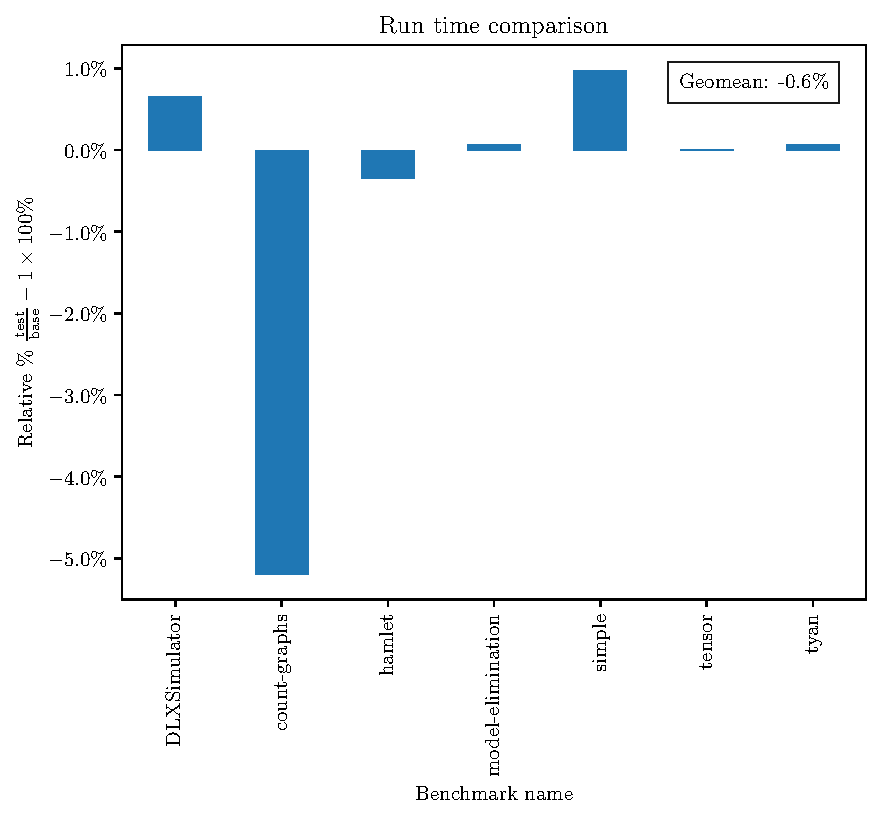
\includegraphics[width=\textwidth]{../analysis/charts/tuple_mlton_run_mlton_vs_mlton.pdf}
    \caption{Run time}
    \label{fig:tuple_mlton_run_mlton_vs_mlton}
  \end{subfigure}
  \hfill
  \begin{subfigure}[b]{0.32\textwidth}
    \centering
    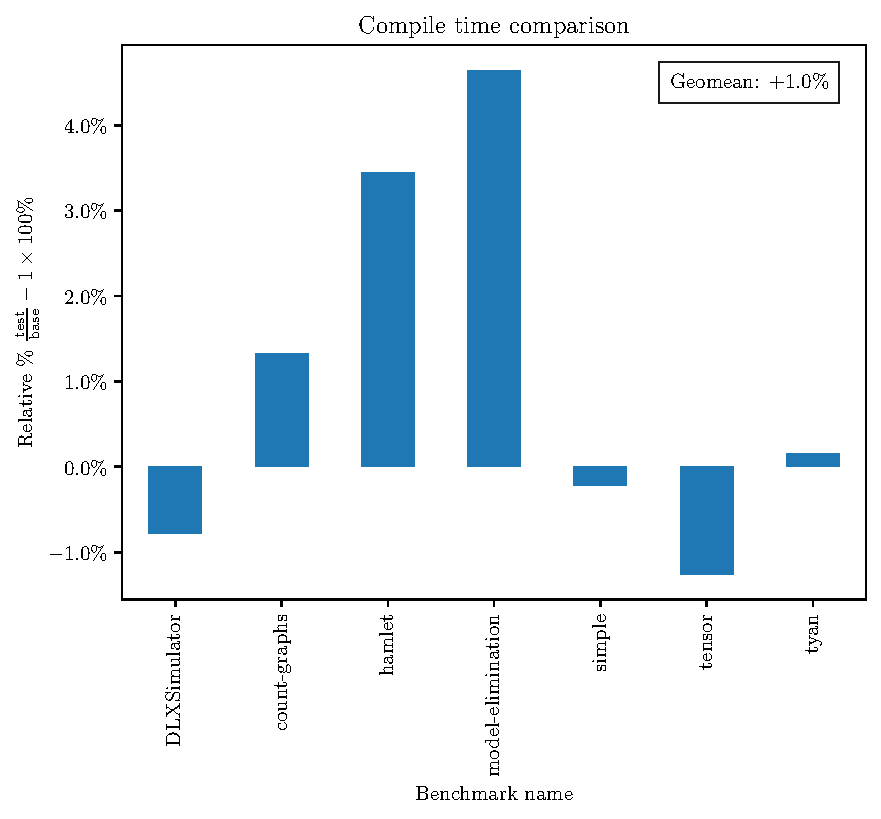
\includegraphics[width=\textwidth]{../analysis/charts/tuple_mlton_compile_mlton_vs_mlton.pdf}
    \caption{Compile time}
    \label{fig:tuple_mlton_compile_mlton_vs_mlton}
  \end{subfigure}
  \hfill
  \begin{subfigure}[b]{0.32\textwidth}
    \centering
    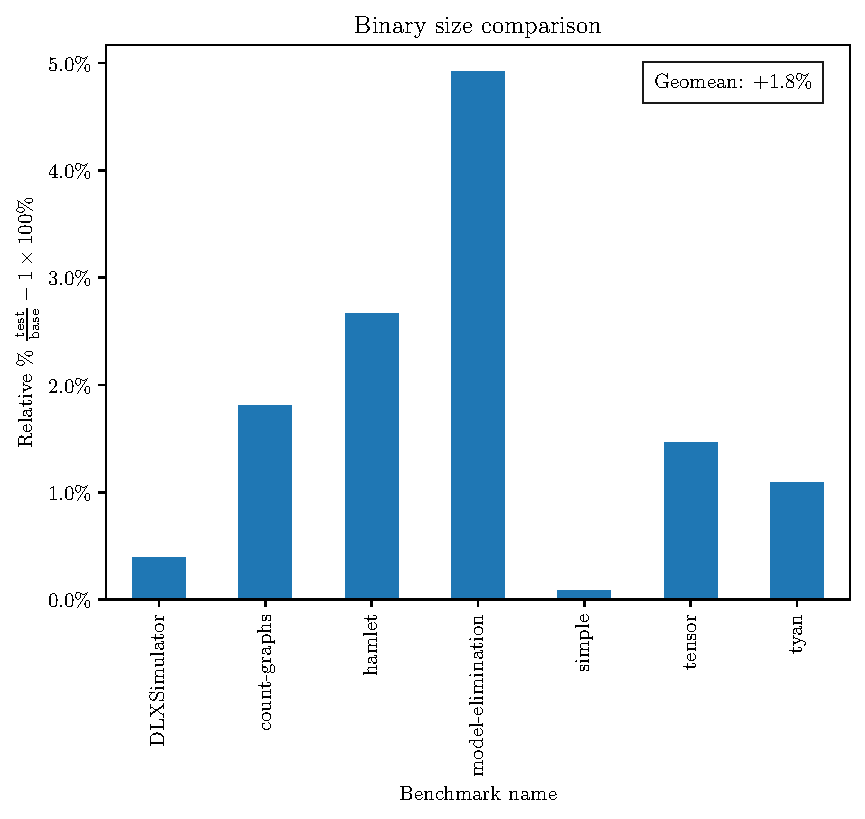
\includegraphics[width=\textwidth]{../analysis/charts/tuple_mlton_size_mlton_vs_mlton.pdf}
    \caption{Binary size}
    \label{fig:tuple_mlton_size_mlton_vs_mlton}
  \end{subfigure}
  \caption{Relative performance for with- vs without-\texttt{PreFlatten} on the MLton benchmark suite. <0\% represents an improvement, >0\% represents a regression.}
  \label{fig:tuple_mlton}
\end{figure}

As seen in \cref{fig:tuple_mlton}, the tuple flattning optimization is broadly
neutral for MLton on the MLton benchmark suite, with <5\% impact on all metrics.

\subsection{\texttt{parallel-ml-bench}: MLton vs MLton}

\begin{figure}[htbp]
  \centering
  \begin{subfigure}[b]{0.48\textwidth}
    \centering
    \includegraphics[width=\textwidth]{../analysis/charts/tuple_parallel_bench_run_mlton_vs_mlton.pdf}
    \caption{Run time}
    \label{fig:tuple_parallel_bench_run_mlton_vs_mlton}
  \end{subfigure}
  \hfill
  \begin{subfigure}[b]{0.48\textwidth}
    \centering
    \includegraphics[width=\textwidth]{../analysis/charts/tuple_parallel_bench_size_mlton_vs_mlton.pdf}
    \caption{Binary size}
    \label{fig:tuple_parallel_bench_size_mlton_vs_mlton}
  \end{subfigure}
  \caption{Relative performance for with- vs without-\texttt{PreFlatten}, applied to tuple constructors on the \texttt{parallel-ml-bench} benchmark suite. <0\% represents an improvement, >0\% represents a regression.}
  \label{fig:tuple_parallel_bench}
\end{figure}

As in the previous section, the impact of the tuple optimization on MLton for
parallel ML bench is also broadly neutral, as seen in
\cref{fig:tuple_parallel_bench}.

One exception is \texttt{reverb}, which shows a huge (40\%) confidence interval.
Examining the raw data in \cref{fig:reverb_tuple_scatter} makes it clear that
both the base and test sides exhibit extreme run-to-run variance (more than a
factor of 2) and so the noise is inherent to the benchmark rather than a new
effect of the tuple flattening optimzation.

\begin{figure}[htbp]
  \centering
  \includegraphics[width=\textwidth]{../analysis/charts/reverb_mlton_parallel_ml_bench_scatter.pdf}
  \caption{Trial-by-trial execution time for \texttt{reverb} in the \texttt{tuple}-flattening configuration.}
  \label{fig:reverb_tuple_scatter}
\end{figure}


\subsection{\texttt{parallel-ml-bench}: MPL vs MPL}

\begin{figure}[htbp]
  \centering
  \begin{subfigure}[b]{0.48\textwidth}
    \centering
    \includegraphics[width=\textwidth]{../analysis/charts/tuple_parallel_bench_run_mpl_vs_mpl_trellis.pdf}
    \caption{Run time}
    \label{fig:tuple_parallel_bench_run_mpl_vs_mpl}
  \end{subfigure}\hfill
  \begin{minipage}[b]{0.48\textwidth}
    \begin{subfigure}{\textwidth}
      \centering
      \includegraphics[width=\textwidth]{../analysis/charts/tuple_parallel_bench_run_mpl_vs_mpl_geomean.pdf}
      \caption{Geomean only}
      \label{fig:tuple_parallel_bench_geomean_mpl_vs_mpl}
    \end{subfigure}

    \begin{subfigure}{\textwidth}
      \centering
      \includegraphics[width=\textwidth]{../analysis/charts/tuple_parallel_bench_size_mpl_vs_mpl.pdf}
      \caption{Binary size}
      \label{fig:tuple_parallel_bench_size_mpl_vs_mpl}
    \end{subfigure}
  \end{minipage}
  \caption{Relative performance for with- vs without-\texttt{PreFlatten}, applied to tuple constructors on the \texttt{parallel-ml-bench} benchmark suite, for the MPL compiler, at a variety of core counts. <0\% represents an improvement, >0\% represents a regression.}
  \label{fig:tuple_parallel_bench_mpl}
\end{figure}

As we see in \cref{fig:tuple_parallel_bench_mpl}, the \texttt{tuple}
optimization has a mixed effect, with some benchmarks showing consistent wins
across core counts, and others showing losses. In order to further investigate
this effect, we'll select two representative benchmarks: \texttt{bfs} (a
consistent win) and \texttt{delaunay} (a consistent loss).

\subsection{\texttt{delaunay} vs \texttt{bfs}: observed IR change}

The \texttt{delaunay} benchmark solves the computational geometry problem of
\textit{Delaunay triangulation}, which partitions the convex hull of a set of
points into triangles whose smallest angles are maximal. In \texttt{delaunay},
the pass flattens arguments to 3 called functions (via duplication):

\begin{enumerate}
\item \texttt{flushArr}: part of the implementation of the \texttt{print} function
\item \texttt{makeTreeBounded}: part of the initialization logic, not included
  in the benchmarked region.
\item \texttt{parfor}: Transforms one branch of MPL's parallel \texttt{for} loop
  construct, going from:

\begin{minted}{python}
  # Parallel for loop on the range (lo, hi) with parallel grain size `grain`
  def parfor(f: 'a -> 'b, lo_hi: int * int, grain: int):
    (lo, hi) = lo_hi # unpack tuple
    # ...end conditions...
    # recursive spawn
    mid = lo + (hi - lo) / 2
    def left():
      parfor (f, (lo, mid), grain)
    def right():
      parfor (f, (mid, hi), grain)
    # launch left + right in parallel
    par (left, right)
\end{minted}
and flattening one of the two \texttt{parfor} recursive calls, i.e.:
\begin{minted}{python}
  # Parallel for loop on the range (lo, hi) with parallel grain size `grain`
  def parfor(f: 'a -> 'b, lo_hi: int * int, grain: int):
    (lo, hi) = lo_hi # unpack tuple
    # ...end conditions...
    # recursive spawn
    mid = lo + (hi - lo) / 2
    def left():
      parfor (f, (lo, mid), grain)
    def right():
      parfor_flat (f, mid, hi, grain)  # flattened recursive call
    # launch left + right in parallel
      par (left, right)

  # flattened specialization of `parfor`
  def parfor_flat(f: 'a -> b, lo: int, hi: int, grain: int): ...
    # ...end conditions...
    # recursive spawn
    mid = lo + (hi - lo) / 2
    def left():
      # construct tuple for unflattened call
      lohi = (lo, mid)
      parfor (f, lo_hi, grain)
    def right():
      parfor_flat (f, mid, hi, grain)  # flattened recursive call
    # launch left + right in parallel
    par (left, right)
\end{minted}
\end{enumerate}

Based on the action of the transformation, we would probably expect to see (for
\texttt{delaunay}):
\begin{enumerate}
\item A small win inside of \texttt{parfor} calls: while we could imagine the
  duplication adding some overhead due to instruction cache effects, the
  duplicated code is fairly small.

\item More-or-less no impact on any other part of the benchmark (test setup and
  \texttt{print} shouldn't have any impact on the per-trial runtime).
\end{enumerate}

%% Doing some arithmetic with the benchmark configuration, we can estimate on the
%% order of 500,000 calls to \texttt{parfor}, and so a $\approx 1$ \mu sec change
%% in this function's performance (which seems like a conservative upper bound for
%% the performance impact of the IR transformation above) should yield a change of
%% $\approx .5$ seconds of CPU time over the full benchmark (on the order of 7\%
%% out of the benchmark's full $\approx 7$ second runtime).

A savings materialized in \texttt{parfor} is consistent with what we see in the
benchmark: overhead in \texttt{parfor} adds delay in spwaning new tasks, and so
we would expect a larger savings at higher core counts. However, the consistent
loss at lower core counts is hard to explain on the basis of the observed IR
transformation.

In the \texttt{bfs} benchmark, the program calculates the BFS tree of an input
graph (i.e. the undirected distance between some distinguished source node and
all other nodes in the graph). The pass applies the following transformations to
\texttt{bfs}:
\begin{enumerate}
\item \texttt{parfor}: the same inline-the-right-hand-branch as above

\item \texttt{parVisitMany}: structurally identical to \texttt{parfor}, manages
  parallel fanout across graph nodes based on their indices

\item \texttt{sumOfOutDegrees}: avoids constructing a temporary tuple to pass as
  an argument to a paralllel reduce operation, roughly:

\begin{minted}{python}
  def sumOfOutDegrees(all_nodes: int array):
    def do_reduce(env: (...complex, 7-element tuple type...)):
      ... calculate sum ...
    reduce(do_reduce, all_nodes)
\end{minted}

where we flatten the \texttt{do\_reduce} call and avoid building the intermediate
\texttt{env} argument.

\end{enumerate}

These changes seem broadly consistent with the observed data, apart from the
observation that the win disappears at higher core counts: given the large error
bars, we can probably explain that effect as either pure noise, or changed GC
behavior (since GC pauses show up as outliers in the trial data).

Next, we'll dig into these results in more detail in order to further explain
the observed trends.


%% \hl{TODO: descibe that they change irrelevant portions}

\subsection{\texttt{delaunay} vs \texttt{bfs}: microarchitectural effects}
A first quick test is to run the microbenchmarks under \texttt{perf} and observe
what (if any) microarchitectural bottlenecks have shifted under the
transformation: did we introduce extra memory traffic, causing the workload to
become backend-bound? Did we introduce code bloat that caused the workload to
become backend bound? One standard methodology for analyzing CPU performance
counter events in order to draw these conflusions is the ``top-down'' method,
introduced by \citet{topdown-paper}, and now supported by the standard Linux
\texttt{perf} tool. The data in this section was collected by running:
\begin{minted}{bash}
  $ perf stat -dd -D $DELAY ... benchmark invocation...
\end{minted}
with the value \texttt{\$DELAY} manually adjusted in order to exclude benchmark
initialization.


Beginning with \texttt{delaunay}, we have, for a single core (in \cref{tab:perf_comparison_delaunay_1core}):
    \begin{table}[htbp]
      \centering
      \caption{Performance metric comparison on 1 core (Delaunay, 1 core)}
      \label{tab:perf_comparison_delaunay_1core}
      \begin{tabular}{lrrr}
        \toprule
        \textbf{Metric} & \textbf{Baseline} & \textbf{Test} & \textbf{Diff / Change} \\
        \midrule
        \multicolumn{4}{l}{\textit{Execution Overview}} \\
        \quad Task Clock (s)           & 148.68 s   & 159.66 s   & +7.39\%   \\
        \quad Instructions ($10^9$)    & 410.49 B   & 464.52 B   & +13.16\%  \\
        \quad IPC                      & 0.90       & 0.98       & +8.89\%   \\
        \midrule
        \multicolumn{4}{l}{\textit{Rates and Miss Percentages}} \\
        \quad Branch Miss Rate         & 2.6\%      & 2.6\%      & 0.0 pp    \\
        \quad L1 D-Cache Miss Rate     & 10.6\%     & 9.3\%      & -1.3 pp   \\
        \quad LLC Load Miss Rate       & 15.8\%     & 15.5\%     & -0.3 pp   \\
        \quad dTLB Load Miss Rate      & 2.3\%      & 2.0\%      & -0.3 pp   \\
        \midrule
        \multicolumn{4}{l}{\textit{Topdown L1 Metrics}} \\
        \quad Retiring                 & 0.9\%      & 1.0\%      & +0.1 pp   \\
        \quad Bad Speculation          & 97.3\%     & 97.3\%     & 0.0 pp    \\
        \quad Frontend Bound           & 0.0\%      & 0.0\%      & 0.0 pp    \\
        \quad Backend Bound            & 1.8\%      & 1.7\%      & -0.1 pp   \\
        \bottomrule
      \end{tabular}
    \end{table}
where \texttt{pp} indicates the absolute difference in percentage points.
Examining the same benchmark at 160 cores, we get (in \cref{tab:perf_comparison_delaunay_160cores}):
\begin{table}[htbp]
  \centering
  \caption{Performance metric comparison on 160 cores (Delaunay, 160 cores)}
  \label{tab:perf_comparison_delaunay_160cores}
  \begin{tabular}{lrrr}
    \toprule
    \textbf{Metric} & \textbf{Baseline} & \textbf{Test} & \textbf{Diff / Change} \\
    \midrule
    \multicolumn{4}{l}{\textit{Execution Overview}} \\
    \quad Task Clock (s)           & 427.34 s   & 423.15 s   & -0.98\%   \\
    \quad Instructions ($10^9$)    & 1024.59 B  & 1048.69 B  & +2.35\%   \\
    \quad IPC                      & 0.82       & 0.85       & +3.66\%   \\
    \midrule
    \multicolumn{4}{l}{\textit{Rates and Miss Percentages}} \\
    \quad Branch Miss Rate         & 0.7\%      & 0.8\%      & +0.1 pp   \\
    \quad L1 D-Cache Miss Rate     & 8.3\%      & 8.0\%      & -0.3 pp   \\
    \quad LLC Load Miss Rate       & 17.7\%     & 18.0\%     & +0.3 pp   \\
    \quad dTLB Load Miss Rate      & 0.6\%      & 0.6\%      & 0.0 pp    \\
    \midrule
    \multicolumn{4}{l}{\textit{Topdown L1 Metrics}} \\
    \quad Retiring                 & 9.6\%      & 11.3\%     & +1.7 pp   \\
    \quad Bad Speculation          & 60.0\%     & 58.5\%     & -1.5 pp   \\
    \quad Frontend Bound           & 8.1\%      & 8.8\%      & +0.7 pp   \\
    \quad Backend Bound            & 22.3\%     & 21.4\%     & -0.9 pp   \\
    \bottomrule
  \end{tabular}
\end{table}
This allows us to draw the following conclusions:
\begin{itemize}
\item On an instruction-for-instruction basis, the \texttt{tuple} transformation
  increases efficiency: both instructions per cycle and the fraction of retiring
  instructions increase between the base and test side.
\item The \texttt{tuple} transformation increases the total instruction count
  required to complete the benchmark by a sufficiently-large amount to balance
  out the IPC improvement (for 1 core).
\item Single-threaded performance is dominated by branch predictor effects, with
  a shocking 97\% of utilization lost to bad speculation. At the full core
  count, the bottleneck shifts towards memory, with a larger fraction of CPU
  time spent waiting on memory (the ``backend bound'' increase).
\item \hl{TODO: MISS RATE METRICS?}
\end{itemize}

Next, for \texttt{bfs}, at one core we have (in \cref{tab:perf_comparison_bfs_1core}):
\begin{table}[htbp]
  \centering
  \caption{Performance metric comparison on 1 core (BFS, 1 core)}
  \label{tab:perf_comparison_bfs_1core}
  \begin{tabular}{lrrr}
    \toprule
    \textbf{Metric} & \textbf{Baseline} & \textbf{Test} & \textbf{Diff / Change} \\
    \midrule
    \multicolumn{4}{l}{\textit{Execution Overview}} \\
    \quad Task Clock (s)           & 172.59 s   & 164.21 s   & -4.86\%   \\
    \quad Instructions ($10^9$)    & 320.10 B   & 326.58 B   & +2.03\%   \\
    \quad IPC                      & 0.62       & 0.67       & +8.06\%   \\
    \midrule
    \multicolumn{4}{l}{\textit{Rates and Miss Percentages}} \\
    \quad Branch Miss Rate         & 1.4\%      & 1.4\%      & 0.0 pp    \\
    \quad L1 D-Cache Miss Rate     & 8.6\%      & 8.7\%      & +0.1 pp   \\
    \quad LLC Load Miss Rate       & 51.3\%     & 51.0\%     & -0.3 pp   \\
    \quad dTLB Load Miss Rate      & 2.7\%      & 2.8\%      & +0.1 pp   \\
    \midrule
    \multicolumn{4}{l}{\textit{Topdown L1 Metrics}} \\
    \quad Retiring                 & 1.1\%      & 1.2\%      & +0.1 pp   \\
    \quad Bad Speculation          & 90.9\%     & 90.3\%     & -0.6 pp   \\
    \quad Frontend Bound           & 0.0\%      & 0.0\%      & 0.0 pp    \\
    \quad Backend Bound            & 7.9\%      & 8.5\%      & +0.6 pp   \\
    \bottomrule
  \end{tabular}
\end{table}
and at 160 cores (in \cref{tab:perf_comparison_bfs_160cores}):
\begin{table}[htbp]
  \centering
  \caption{Performance metric comparison on 160 cores (BFS, 160 cores)}
  \label{tab:perf_comparison_bfs_160cores}
  \begin{tabular}{lrrr}
    \toprule
    \textbf{Metric} & \textbf{Baseline} & \textbf{Test} & \textbf{Diff / Change} \\
    \midrule
    \multicolumn{4}{l}{\textit{Execution Overview}} \\
    \quad Task Clock (s)           & 822.65 s   & 816.26 s   & -0.78\%   \\
    \quad Instructions ($10^9$)    & 1454.22 B  & 1423.12 B  & -2.14\%   \\
    \quad IPC                      & 0.61       & 0.60       & -1.64\%   \\
    \midrule
    \multicolumn{4}{l}{\textit{Rates and Miss Percentages}} \\
    \quad Branch Miss Rate         & 0.6\%      & 0.7\%      & +0.1 pp   \\
    \quad L1 D-Cache Miss Rate     & 7.8\%      & 8.0\%      & +0.2 pp   \\
    \quad LLC Load Miss Rate       & 44.6\%     & 44.7\%     & +0.1 pp   \\
    \quad dTLB Load Miss Rate      & 1.2\%      & 1.3\%      & +0.1 pp   \\
    \midrule
    \multicolumn{4}{l}{\textit{Topdown L1 Metrics}} \\
    \quad Retiring                 & 3.3\%      & 3.0\%      & -0.3 pp   \\
    \quad Bad Speculation          & 77.0\%     & 79.7\%     & +2.7 pp   \\
    \quad Frontend Bound           & 1.2\%      & 1.2\%      & 0.0 pp    \\
    \quad Backend Bound            & 18.6\%     & 16.1\%     & -2.5 pp   \\
    \bottomrule
  \end{tabular}
\end{table}
Here, we can see:
\begin{itemize}
\item While we still have instruction bloat, the increase to IPC / retiring
  pipeline slots was large enough to improve performance overall (showing as a
  decrease in ``Task Clock'').
\item This benchmark still suffers from extreme utilization loss due to bad speculation.
\item \hl{TODO: miss rates?}
\end{itemize}

On the whole, the microarchitectural data is not particularly enlightening in
terms of understanding the output of the \texttt{tuple} transformation: the main
interesting finding here is that the generated code evidently interacts
extremely poorly with the CPU's branch predictor.

Briefly examining the poor branch predictor behavior: one potential hypothesis
is that the observed behavior is the result of the heavy use of the jump table
structure of the generated C code described above. We can drill down into this
further by examinining the types of mispredicted branches: conditional
(taken/not-taken) vs indirect. If the high mispredict rate is a consequence of
the jump table structure in the emitted C, we would expect to see it manifest as
a high mispredict rate for indirect branches. If, on the other hand, the high
mispredict rate is simply a property of how the algorithm operates on the input
data, we would expect to see a high rate of mispredictions for conditional
branches.

Measuring using the lower-level \texttt{perf} events, we get the following data
(in \cref{tab:badspec_hierarchical_tuple}):
\begin{table}[htbp]
  \centering
  \caption{Branch mispredictions breakdown as a percentage of total mispredictions, for the \texttt{tuple} configuration.}
  \label{tab:badspec_hierarchical_tuple}
  \begin{tabular}{lrr}
    \toprule
    \textbf{Branch Type} & \textbf{Delaunay (1 core)} & \textbf{BFS (1 core)} \\
    \midrule
    \textbf{Conditional (Total)} & \textbf{95.32\%} & \textbf{99.87\%} \\
    \quad Taken                  & 52.41\%          & 48.45\%          \\
    \quad Not-taken              & 42.91\%          & 51.42\%          \\
    \textbf{Indirect}            &  \textbf{4.64\%} &  \textbf{0.06\%} \\
    \textbf{Return (\texttt{ret})}& \textbf{0.04\%} &  \textbf{0.08\%} \\
    \bottomrule
  \end{tabular}
\end{table}
Given that nearly all mispredictions are conditional rather than indirect, we
can conclude that the high mispredict rate is an inherent property of the
algorithm and the input data rather than a deficiency of MLton codegen.


\subsection{\texttt{delaunay} vs \texttt{bfs}: control for known effects}
Another strategy we can use to understand how the pass impacted performance
(trying to compensate for the lack of source-level profiling with MPL that we
might use to understand performance in another language) is to try to separate
out the actual intended change implemented by the pass (as described above) from
other downstream effects.

Digging more deeply into the action of the pass, we can identify three direct
consequences:
\begin{enumerate}
\item The actual function duplication/tuple-flattening change (described above).

\item The post-change IR cleanup, running the generic MLton \texttt{Simplify}
  pass to perform optimizations after flattening: perhaps the \texttt{tuple}
  optimization itself is unhelpful, and the win is just from running
  \texttt{Simplify} again. We can control for this by running \texttt{Simplify}
  on both the baseline and the test.

\item Later on, during the \texttt{Chunkify} pass, introducing the new,
  flattened functions: perhaps the \texttt{tuple} optimization's change to tuple
  layout has no direct impact, but the new functions happen to move around chunk
  boundaries in a way that is helpful/unhelpful. We can control for this by
  using the compiler flag \texttt{-chunkify one} to force all functions into a
  single C chunk (improving performance at the cost of C compile time).

\end{enumerate}

In \cref{fig:tuple_standouts_only}, we see the impact of these three different
configurations: the relative performance when enabling ``baseline fixup'' is
generally the same as our standard experimental configuration, the performance
under \texttt{-chunkify one} is virtually identical between the baseline and the
test.

Therefore, on these two benchmarks, the actual transformation of the pass has
nearly zero impact on performance: the most important driver of performance
changes is simply the accidental permutation of chunk boundaries by creating new
functions. Looking at a comparison of the geomeans across all benchmarks in
\cref{fig:tuple_exp_geomeans} broadly confirms that this observation holds
across the entire benhcmark suite, showing roughly identical performance between
the regular configuration and the with-baseline-fixup configuration, and
neutral-to-positive impact from tuple flattening.

See the full set of benchmark data for \texttt{-chunkify one} in
\cref{fig:tuple_all_chunkify_one}. This data indicates that while the
transformation does appear to have a significant impact on a handful of
benchmarks (\texttt{ocaml-lu-decomp}, \texttt{tokens}), it is otherwise
neutral-to-positive, with an impact of $< 2\%$ on performance in most cases.


\begin{figure}[htbp]
  \centering
  \begin{subfigure}[b]{0.48\textwidth}
    \centering
    \includegraphics[width=\textwidth]{../analysis/charts/tuple_exp_bfs.pdf}
    \caption{\texttt{bfs}}
    \label{fig:tuple_exp_bfs}
  \end{subfigure}
  \hfill
  \begin{subfigure}[b]{0.48\textwidth}
    \centering
    \includegraphics[width=\textwidth]{../analysis/charts/tuple_exp_delaunay.pdf}
    \caption{\texttt{delaunay}}
    \label{fig:tuple_exp_delaunay}
  \end{subfigure}
  \caption{Comparison of speedups across core counts for \texttt{bfs} and \texttt{delaunay} under three configurations: baseline tuple-vs-tuple, baseline with fixup, and with \texttt{-chunkify one}. <0\% represents an improvement, >0\% represents a regression.}
  \label{fig:tuple_standouts_only}
\end{figure}

\begin{figure}[htbp]
  \centering
  \includegraphics[width=\textwidth]{../analysis/charts/tuple_exp_geomeans.pdf}
  \caption{Comparison of geometric mean speedups across core counts for the baseline tuple configuration, baseline with fixup, and with \texttt{-chunkify one}. <0\% represents an improvement, >0\% represents a regression.}
  \label{fig:tuple_exp_geomeans}
\end{figure}

\begin{figure}[htbp]
  \centering
  \includegraphics[width=\textwidth,height=0.88\textheight,keepaspectratio]{../analysis/charts/tuple_chunkify_one_parallel_bench_run_mpl_vs_mpl_trellis.pdf}
  \caption{Relative performance for tuple flattening with \texttt{-chunkify one} on the \texttt{parallel-ml-bench} benchmark suite, for the MPL compiler, across core counts. <0\% represents an improvement, >0\% represents a regression.}
  \label{fig:tuple_all_chunkify_one}
\end{figure}

%% \hl{TODO: Look at output from chunkify one. Conclude that chunkify is the
%%   culprit. Link to an appendix with the full table of results from these
%%   experiments and conclude that there are more unexplained effects}.

%% As seen in \cref{fig:tuple_parallel_bench_mpl}, the \texttt{tuple} optimization
%% is a fairly consistent loss across the benchmark suite; with the most striking
%% example \texttt{dense-matmul} displaying a 30\% loss for lower core count tests.

%% \hl{TODO: NEED ANALYSIS. MAYBE HYPERTHREADING IS RELEVANT?}

\FloatBarrier
\section{\texttt{ConApp} Flattening}

For the evaluation below, we use the following configuration:

\begin{itemize}
\item \texttt{PreFlatten} runs before \texttt{Flatten} (so that \texttt{Flatten}
  has the chance to optimize away the tuples that remain after eliding the ADT
  tags)

\item \texttt{PreFlatten} transforms all functions (both tail-recurisve and not)

\item \texttt{PreFlatten} runs 10 ``recurisve steps'' (\hl{TODO: LIKE ABOVE?})
\end{itemize}

\subsection{MLton Benchmarks}

\begin{figure}[htbp]
  \centering
  \begin{subfigure}[b]{0.32\textwidth}
    \centering
    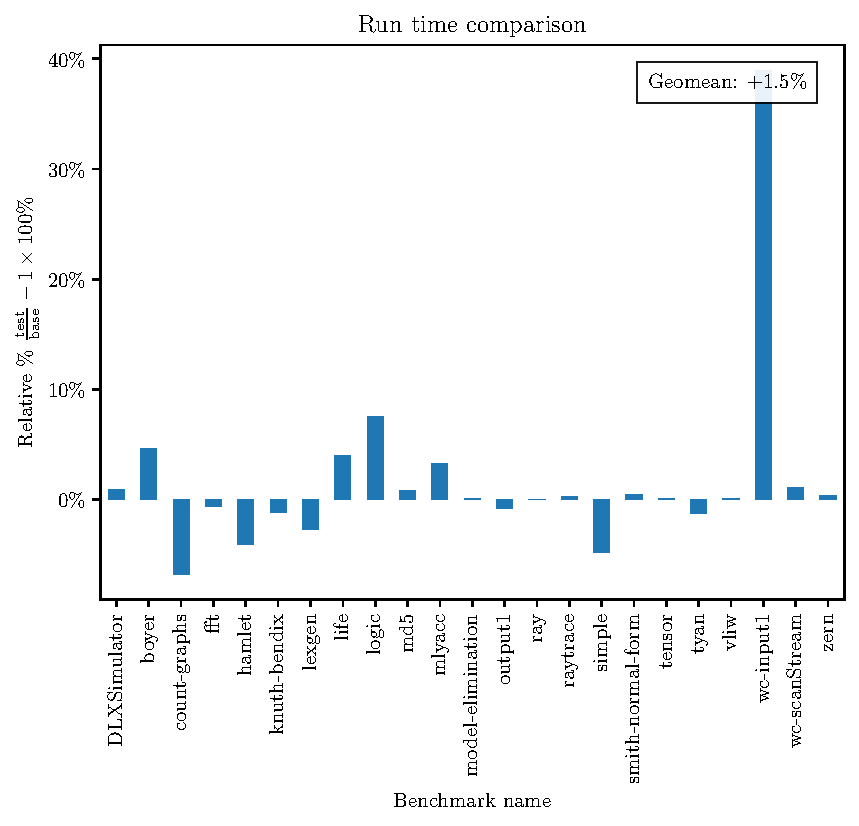
\includegraphics[width=\textwidth]{../analysis/charts/con_mlton_run_mlton_vs_mlton.pdf}
    \caption{Run time}
    \label{fig:con_mlton_run_mlton_vs_mlton}
  \end{subfigure}
  \hfill
  \begin{subfigure}[b]{0.32\textwidth}
    \centering
    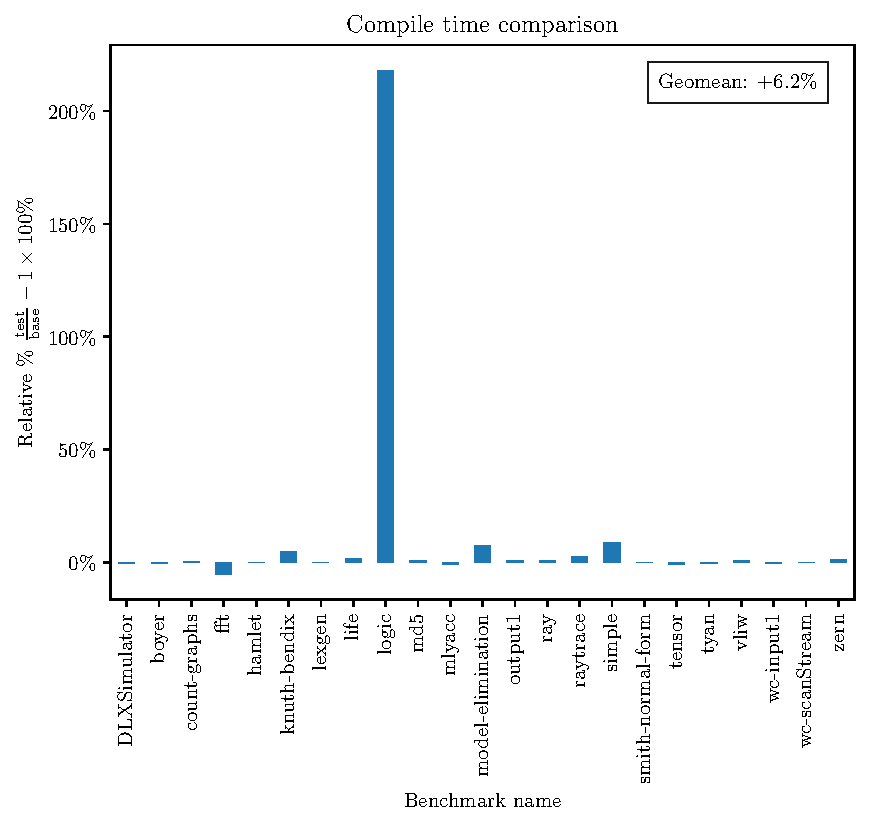
\includegraphics[width=\textwidth]{../analysis/charts/con_mlton_compile_mlton_vs_mlton.pdf}
    \caption{Compile time}
    \label{fig:con_mlton_compile_mlton_vs_mlton}
  \end{subfigure}
  \hfill
  \begin{subfigure}[b]{0.32\textwidth}
    \centering
    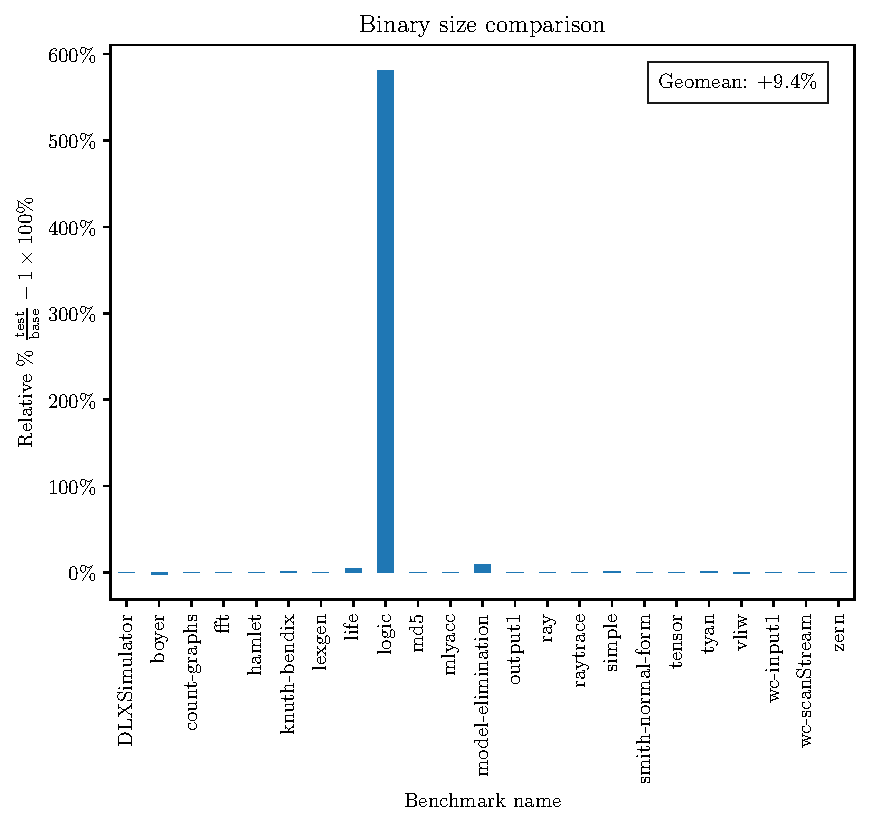
\includegraphics[width=\textwidth]{../analysis/charts/con_mlton_size_mlton_vs_mlton.pdf}
    \caption{Binary size}
    \label{fig:con_mlton_size_mlton_vs_mlton}
  \end{subfigure}
  \caption{Relative performance for with- vs without-\texttt{PreFlatten}, applied to \texttt{ConApp} on the MLton benchmark suite. <0\% represents an improvement, >0\% represents a regression.}
  \label{fig:con_mlton}
\end{figure}

\hl{TODO: THIS IS NOW A WIN}

The MLton benchmark suite shows modest $\approx 5\%$ regressions on a number of
benchmarks, for an overall geomean loss. We'll investiage the large loss to
\texttt{wc-input1} in the next section.

\subsection{\texttt{wc-input1}: detailed analysis}

The benchmark itself is simply a loop that reads from a buffered IO stream and
counts newlines:
\begin{minted}{sml}
fun loop (i: int): int =
  case input1 ins of
    NONE => i
  | SOME c => loop (if c = #"\n" then i + 1 else i)
\end{minted}
where \texttt{input1} is a standard library function that reads a single
character from a provided input stream (here, a temporary file).

The \texttt{ConApp} flattening pass makes the following changes:
\begin{itemize}
\item During initialization, it flattens the call to a string-concatenation routine
\item During runtime, it flattens calls to various functions that report errors
  in case of e.g. IO failure when reading the file.
\end{itemize}
No hot codepaths whatsoever are impacted. What is the cause of the regression?

Like above, we can run in \texttt{-chunkify one} in order to control for the
effect of chunkification, which is impacted by the introduction of any new
functons.

\hl{TODO: THE DATA CHANGED AND WE NEED TO REWORK THE ANALYSIS A BIT}

\FloatBarrier
\section{\texttt{wc-input1}: controlling for \texttt{Chunkify}}

As we can see in \cref{fig:mlton_bench_mlton_con_chunkify_one}, nearly the
entire positive effect of the transformation observed on the MLton benchmark
suite is actually due to accidental permutation of chunk boundaries rather than
the inded purpose of the pass -- the majr wins on \texttt{wc-input1} and
\texttt{wc-scanStream} disappear, and we are left with a small geomean loss
rather than a win.

\begin{figure}[htbp]
  \centering
  \includegraphics[width=\textwidth,keepaspectratio]{../analysis/charts/mlton_con_chunkify_one_mlton_bench.pdf}
  \caption{Comparison of benchmark performance for \texttt{ConApp} flattening on the MLton benchmark suite under MLton, comparing the baseline configuration against \texttt{-chunkify one}. <0\% represents an improvement, >0\% represents a regression.}
  \label{fig:mlton_bench_mlton_con_chunkify_one}
\end{figure}


\FloatBarrier
\section{\texttt{parallel-ml-bench}: MLton vs MLton}

\begin{figure}[htbp]
  \centering
  \begin{subfigure}[b]{0.48\textwidth}
    \centering
    \includegraphics[width=\textwidth]{../analysis/charts/con_parallel_bench_run_mlton_vs_mlton.pdf}
    \caption{Run time}
    \label{fig:con_parallel_bench_run_mlton_vs_mlton}
  \end{subfigure}
  \hfill
  \begin{subfigure}[b]{0.48\textwidth}
    \centering
    \includegraphics[width=\textwidth]{../analysis/charts/con_parallel_bench_size_mlton_vs_mlton.pdf}
    \caption{Binary size}
    \label{fig:con_parallel_bench_size_mlton_vs_mlton}
  \end{subfigure}
  \caption{Relative performance for with- vs without-\texttt{PreFlatten}, applied to \texttt{ConApp} on the \texttt{parallel-ml-bench} benchmark suite. <0\% represents an improvement, >0\% represents a regression.}
  \label{fig:con_parallel_bench}
\end{figure}

On \cref{fig:con_parallel_bench}, we see strong wins across a number of
benchmarks, and few losses, for a strong geomean win of $4.1\%$. To what degree
is this measurement impacted by chunkification noise, as we saw above?

The chart \cref{fig:con_parallel_bench_mlton_chunkify} plots the relative
performance of the default experimental setup alongside the relative performance
in a setup with \texttt{-chunkify one}. As we can see, the largest wins in
\texttt{linearrec} and \texttt{quickhull} persist: this suggests an
individually-meaningful impact of the \texttt{ConApp} flattening transformation,
unlike the \texttt{tuple} case.

However, it surfaces one significant loss on \texttt{mcss-opt} that likely
requires further investigation. We also see a number of significant wins
disappear (e.g. \texttt{primes} and \texttt{sparse-mxv-opt}), suggesting that
the baseline measurement does contain significant incidental performance changes
due to chunkification.

\begin{figure}[htbp]
  \centering
  \includegraphics[width=\textwidth,keepaspectratio]{../analysis/charts/mlton_con_chunkify_one_parallel_bench.pdf}
  \caption{Comparison of benchmark performance for \texttt{ConApp} flattening on \texttt{parallel-ml-bench} under MLton, comparing the baseline configuration against \texttt{-chunkify one}. <0\% represents an improvement, >0\% represents a regression.}
  \label{fig:con_parallel_bench_mlton_chunkify}
\end{figure}

\subsection{\texttt{parallel-ml-bench}: MPL vs MPL}

\begin{figure}[htbp]
  \centering
  \begin{subfigure}[b]{0.48\textwidth}
    \centering
    \includegraphics[width=\textwidth]{../analysis/charts/con_parallel_bench_run_mpl_vs_mpl_trellis.pdf}
    \caption{Run time}
    \label{fig:con_parallel_bench_run_mpl_vs_mpl}
  \end{subfigure}\hfill
  \begin{minipage}[b]{0.48\textwidth}
    \begin{subfigure}{\textwidth}
      \centering
      \includegraphics[width=\textwidth]{../analysis/charts/con_parallel_bench_run_mpl_vs_mpl_geomean.pdf}
      \caption{Geomean only}
      \label{fig:con_parallel_bench_geomean_mpl_vs_mpl}
    \end{subfigure}

    \begin{subfigure}{\textwidth}
      \centering
      \includegraphics[width=\textwidth]{../analysis/charts/con_parallel_bench_size_mpl_vs_mpl.pdf}
      \caption{Binary size}
      \label{fig:con_parallel_bench_size_mpl_vs_mpl}
    \end{subfigure}
  \end{minipage}
  \caption{Relative performance for with- vs without-\texttt{PreFlatten}, applied to \texttt{ConApp} on the \texttt{parallel-ml-bench} benchmark suite, for the MPL compiler, at a variety of core counts. <0\% represents an improvement, >0\% represents a regression.}
  \label{fig:con_parallel_bench_mpl}
\end{figure}

\hl{UPDATED THE CHARTS: NEED TO RE-CHECK THE BENCHMARK NAMES BELOW}

In the default experiment configuration, we see an overall loss for
\texttt{ConApp} flattening in MPL, driven primarily by a large, consistent
regression against \texttt{suffix-array}.

Re-running this particular benchmark under \texttt{-chunkify one} shows that the
effect disappears, as we can see in \cref{fig:con_chunkify_one_outliers}:
\texttt{suffix-array} is roughly neutral under \texttt{ConApp} flattening once
we control for chunkification. We can also see how the large swings reported by
\texttt{linearrec} change under \texttt{-chunkify one} in
\cref{fig:con_chunkify_one_outliers}: here, it appears that there is a
legitimate effect on the benchmark at higher core counts which merits further
investigation.

\begin{figure}[htbp]
  \centering
  \begin{subfigure}[b]{0.48\textwidth}
    \centering
    \includegraphics[width=\textwidth]{../analysis/charts/con_exp_suffix_array.pdf}
    \caption{\texttt{suffix-array}}
    \label{fig:con_exp_suffix_array}
  \end{subfigure}
  \hfill
  \begin{subfigure}[b]{0.48\textwidth}
    \centering
    \includegraphics[width=\textwidth]{../analysis/charts/con_exp_linearrec.pdf}
    \caption{\texttt{linearrec}}
    \label{fig:con_exp_linearrec}
  \end{subfigure}
  \caption{Comparison of speedups across core counts for \texttt{suffix-array} and \texttt{linearrec} under baseline \texttt{ConApp} flattening versus with \texttt{-chunkify one}. <0\% represents an improvement, >0\% represents a regression.}
  \label{fig:con_chunkify_one_outliers}
\end{figure}

In \cref{fig:con_chunkify_one_geomeans}, we see that (like \texttt{tuple}
flattening), the \texttt{ConApp} flattening transformation is broadly
neutral-to-positive when excluding chunk overhead. See
\cref{fig:mpl_con_chunkify_one_all} for the full set of experimental data for the
\texttt{-chunkify one} configuration.

\begin{figure}[htbp]
  \centering
  \includegraphics[width=\textwidth]{../analysis/charts/con_exp_geomean.pdf}
  \caption{Comparison of geometric mean speedups across core counts for baseline \texttt{ConApp} flattening versus with \texttt{-chunkify one}. <0\% represents an improvement, >0\% represents a regression.}
  \label{fig:con_chunkify_one_geomeans}
\end{figure}

\begin{figure}[htbp]
  \centering
  \includegraphics[width=\textwidth,height=0.88\textheight,keepaspectratio]{../analysis/charts/con_chunkify_one_parallel_bench_run_mpl_vs_mpl_trellis.pdf}
  \caption{Relative performance for \texttt{ConApp} flattening with \texttt{-chunkify one} on the \texttt{parallel-ml-bench} benchmark suite, for the MPL compiler, across core counts. <0\% represents an improvement, >0\% represents a regression.}
  \label{fig:mpl_con_chunkify_one_all}
  \label{mpl_con_chunkify_one_all}
\end{figure}

\FloatBarrier
\section{AoS Flattening}

\hl{TODO: CHECK -- 3 or 4 elements?}

In the data below, we applied the Array-of-Struct \texttt{ShallowFlatten}
transformation to all containers-of-tuples of less than or equal to 3 elements.

\subsection{MLton Benchmarks}

\begin{figure}[htbp]
  \centering
  \begin{subfigure}[b]{0.32\textwidth}
    \centering
    \includegraphics[width=\textwidth]{../analysis/charts/aos_mlton_run_mlton_vs_mlton.pdf}
    \caption{Run time}
    \label{fig:aos_mlton_run_mlton_vs_mlton}
  \end{subfigure}
  \hfill
  \begin{subfigure}[b]{0.32\textwidth}
    \centering
    \includegraphics[width=\textwidth]{../analysis/charts/aos_mlton_compile_mlton_vs_mlton.pdf}
    \caption{Compile time}
    \label{fig:aos_mlton_compile_mlton_vs_mlton}
  \end{subfigure}
  \hfill
  \begin{subfigure}[b]{0.32\textwidth}
    \centering
    \includegraphics[width=\textwidth]{../analysis/charts/aos_mlton_size_mlton_vs_mlton.pdf}
    \caption{Binary size}
    \label{fig:aos_mlton_size_mlton_vs_mlton}
  \end{subfigure}
  \caption{Relative performance for with- vs without-\texttt{ShallowFlatten}, using the AoS transformation on the MLton benchmark suite. <0\% represents an improvement, >0\% represents a regression.}
  \label{fig:aos_mlton}
\end{figure}

As we can see in \cref{fig:aos_mlton}, this transformation is essentially a
no-op on the MLton benchmark suite, impacting only a single benchmark for a win
smaller than 1\%.


\subsection{\texttt{parallel-ml-bench}: MLton vs MLton}

\begin{figure}[htbp]
  \centering
  \begin{subfigure}[b]{0.48\textwidth}
    \centering
    \includegraphics[width=\textwidth]{../analysis/charts/aos_parallel_bench_run_mlton_vs_mlton.pdf}
    \caption{Run time}
    \label{fig:aos_parallel_bench_run_mlton_vs_mlton}
  \end{subfigure}
  \hfill
  \begin{subfigure}[b]{0.48\textwidth}
    \centering
    \includegraphics[width=\textwidth]{../analysis/charts/aos_parallel_bench_size_mlton_vs_mlton.pdf}
    \caption{Binary size}
    \label{fig:aos_parallel_bench_size_mlton_vs_mlton}
  \end{subfigure}
  \caption{Relative performance for with- vs without-\texttt{ShallowFlatten}, using the AoS transformation on the \texttt{parallel-ml-bench} benchmark suite. <0\% represents an improvement, >0\% represents a regression.}
  \label{fig:aos_parallel_bench}
\end{figure}

AOS flattening has a largely poisitive impact on MLton for the
\texttt{parallel\_bench} suite. We'll focus on MPL for a more detailed analysis,
in the style of the previous sections.

\subsection{\texttt{parallel-ml-bench}: MPL vs MPL}

\begin{figure}[htbp]
  \centering
  \begin{subfigure}[b]{0.48\textwidth}
    \centering
    \includegraphics[width=\textwidth]{../analysis/charts/aos_parallel_bench_run_mpl_vs_mpl_trellis.pdf}
    \caption{Run time}
    \label{fig:aos_parallel_bench_run_mpl_vs_mpl}
  \end{subfigure}\hfill
  \begin{minipage}[b]{0.48\textwidth}
    \begin{subfigure}{\textwidth}
      \centering
      \includegraphics[width=\textwidth]{../analysis/charts/aos_parallel_bench_run_mpl_vs_mpl_geomean.pdf}
      \caption{Geomean only}
      \label{fig:aos_parallel_bench_geomean_mpl_vs_mpl}
    \end{subfigure}

    \begin{subfigure}{\textwidth}
      \centering
      \includegraphics[width=\textwidth]{../analysis/charts/aos_parallel_bench_size_mpl_vs_mpl.pdf}
      \caption{Binary size}
      \label{fig:aos_parallel_bench_size_mpl_vs_mpl}
    \end{subfigure}
  \end{minipage}
  \caption{Relative performance for with- vs without-\texttt{ShallowFlatten}, using the AoS transformation on the \texttt{parallel-ml-bench} benchmark suite, for the MPL compiler, at a variety of core counts. <0\% represents an improvement, >0\% represents a regression.}
  \label{fig:aos_parallel_bench_mpl}
\end{figure}

For MPL, the AOS transformation is overwhelmingly positive. For a deep dive,
we'll focus on two cases with large effects: \texttt{quickhull} (a large,
consistent win) and \texttt{linearrec} (a win at low core counts that becomes a
noisy loss at high core counts.

\subsection{\texttt{quickhull}, \texttt{linearrec}: observed IR change}
The \texttt{quickhull} benchmark calculates the convex hull of a 2D set of
points. In the particular implementation used in \texttt{parallel\_ml\_bench},
the core of the algorithm involves filtering a set of indices into two smaller
sets, e.g., very roughly:
\begin{minted}{python}
  points: (float * float) array = ...initialized on startup...
  def partition(indices: int list) -> (int array) * (int array):
    def is_left(index: int) -> bool:
      # Indexed load into `points`
      p: (float * float) = points[index]
      ...some 2D geometry calculation that loads points...

    def is_right(index: int) -> bool:
      ...similar...

    lefts: int list = filter(is_left, indices)
    right: int list = filter(is_right, indices)
    return (filter(is_left, indices), filter(is_right, indices))
  def quickhull(indices: int array, ...) -> int array:
    if len(indices) < C:
      ...base case...
    else:
      left, right = partition(indices)
      left_result = quickhull(left)
      right_result = quickhull(right)
      ...merge...
      return result
\end{minted}

The \texttt{linearrec} benchmark is quite simple, calculating a first-order
linear recurrence across a sequence of 2D points, i.e., in the scalar code:
\begin{minted}{python}
  points: (float * float) array = ...

  def linearrec(points):
    def combine(left: (float * float), right: (float * float)) -> (float * float):
      l_x, l_y = left
      r_x, r_y = right
      return (l_x * r_x, l_y * r_x + r_y)

    def select(point: float * float) -> float:
      l, r = point
      return l

    identity = (1.0, 0.0)
    # Prefix scan over pairs with `combine`
    points' = list(prefix_scan(pairs, combine))
    return [select(p) for p in points']
\end{minted}
where \texttt{prefix\_scan} is an MPL primitive that calculates the parallel
prefix scan of the associative \texttt{combine} operator, i.e. the sequence:
\begin{minted}{python}
  identity = (1.0, 0.0)
  points' = [combine(identity, points[0]),
             combine(points'[0], points[1]),
             combine(points'[1], points[2]),
             ...]
\end{minted}
through a standard paralell prefix scan algorithm that completes the task in
$O(n)$ total work and a critical path length of $O(\log n)$ operations.

The transformations here are straightforward: for \texttt{quickhull}, we rewrite
the global \texttt{points} array into array-of-structs format:
\begin{minted}{python}
  points: float array = ...initialized on startup...
  def partition(indices: int list) -> (int array) * (int array):
    def is_left(index: int) -> bool:
      # Indexed load into `points`
      p_x: float = points[index * 2]
      p_y: float = points[index * 2 + 1]
      # Temporary tuple produced by the `ShallowFlatten` transformation
      p: float * float = (p_x, p_y)
      ...some 2D geometry calculation that loads points...

    def is_right(index: int) -> bool:
      ...similar...

  ...as above...
\end{minted}
where the temporary tuple \texttt{p} is successfully eliminated by later passes,
allowing the 2D geometry calculation operate directly on the unboxed values.

The transformation on \texttt{linearrec} is similarly obvious -- however, the IR
snippet from above remains unchaned because the transformation changes the body
of \texttt{parallel\_scan} to calculate a prefix sum over a flat \texttt{float *
  float} array. Later passes ensure that all temporary tuples are optimized
away, such that \texttt{ShallowFlatten} introduces no new allocations.

One important difference to note between \texttt{linearrec} and
\texttt{quickhull} is that, while \texttt{quickhull} only allocates
arrays-of-tuples at startup, \texttt{linearrec} allocates arrays of tuples at
runtime as well -- temporary arrays while computing the prefix scan. Thus for
\texttt{quickhull}, we observe only the effect of the transformation on the
generated code, but in \texttt{linearrec} we can also observe the interaction
with the garbage collector.



\subsection{\texttt{quickhull}, \texttt{linearrec}: microarchitectural effects}
Next, we walk through the same \texttt{perf}-centered analysis to determine how
the AOS transformation impacted the workload at a microarchitectural level. In
both cases, the effect we expect to see is the one described in the sections
above \hl{TODO LINK TO THE MEAT SECTION} -- in the cases where loading from the
2D point arrays is important for performance, saving the intermediate tuple
should save both memory latency (i.e. an extra dependent load operation --
shortening the chain length from 3 to 2 for \texttt{quickhull} and from 2 to 1
for \texttt{linearrec}) and memory bandwidth (we should be able to use the whole
cacheline that each point is allocated on).

For \texttt{quickhull}, we can see the single-threaded effect in
\cref{tab:perf_comparison_aos_quickhull_1core}. We observe, broadly, the effect
that we expect: we see better locality show up as a lower miss rate in both L1
and L3, translating into higher IPC. In additon to higher IPC, we also see a
reduction in total instructions, matching out expectations (since the packed AOS
loads require fewer instructions than the unpacked tuple loads, so long as the
intermediate tuples are optimized away). \hl{TODO: WHY BAD SPEC? LOWER MISS RATE
  SHOUHD SHOW UP AS LESS BACKEND BOUND}

Comparing with the 160 core data in
\cref{tab:perf_comparison_aos_quickhull_160cores}, trend for \texttt{quickhull}
is similar to the benchmarks we analyzed above, with the microarchitectural
bottleneck shifting from bad speculation towards backend bound as contention on
the memory subsystem increases.

For \texttt{linearrec}, the primary effect we observe in the single core data
from \cref{tab:perf_comparison_aos_linearrec_1core} is a massive reduction in
instruction count, which again corresponds with what we expect based on the
action of the transformation. Here, we see a slightly higher L1 miss rate
alongside a lower L3 miss rate, which we could explain as follows: for the
baseline verison, we tend to keep the pointers-to-tuples in L1 (i.e. the array
of pointers is small and has good locality) and miss in L3 when we load through
the poiners, whereas in the AOS version, the packed array is large enough to
exceed the size of L1, but we still have enough locality to keep it in lower
levels of the cache hierachy.



\hl{TODO: EXPLAIN THE INSTRUCTIONS / IPC / BADSPEC FOR LINEARREC AS GC}

\hl{TODO: DIG INTO THIS FURTHER USING PERF RECORD TO COLLECT THE ACTUAL DATA}

\hl{TODO: WRITEUP}

  1. Quickhull on 1 Core

    \begin{table}[htbp]
      \centering
      \caption{AoS performance metric comparison on 1 core (Quickhull, 1 core)}
      \label{tab:perf_comparison_aos_quickhull_1core}
      \begin{tabular}{lrrr}
        \toprule
        \textbf{Metric} & \textbf{Baseline} & \textbf{Test} & \textbf{Diff / Change} \\
        \midrule
        \multicolumn{4}{l}{\textit{Execution Overview}} \\
        \quad Task Clock (s)           & 49.53 s   & 36.65 s   & -26.00\%   \\
        \quad Instructions ($10^9$)    & 233.33 B  & 175.11 B  & -24.95\%   \\
        \quad IPC                      & 1.59       & 1.61       & +1.26\%    \\
        \midrule
        \multicolumn{4}{l}{\textit{Rates and Miss Percentages}} \\
        \quad Branch Miss Rate         & 1.7\%      & 2.2\%      & +0.5 pp    \\
        \quad L1 D-Cache Miss Rate     & 3.5\%      & 2.2\%      & -1.3 pp    \\
        \quad LLC Load Miss Rate       & 63.5\%     & 48.4\%     & -15.1 pp   \\
        \quad dTLB Load Miss Rate      & 0.1\%      & 0.1\%      & 0.0 pp     \\
        \midrule
        \multicolumn{4}{l}{\textit{Topdown L1 Metrics}} \\
        \quad Retiring                 & 2.6\%      & 5.3\%      & +2.7 pp    \\
        \quad Bad Speculation          & 88.9\%     & 85.6\%     & -3.3 pp    \\
        \quad Frontend Bound           & 0.3\%      & 0.3\%      & 0.0 pp     \\
        \quad Backend Bound            & 8.3\%      & 8.8\%      & +0.5 pp    \\
        \bottomrule
      \end{tabular}
    \end{table}

  2. Quickhull on 160 Cores

    \begin{table}[htbp]
      \centering
      \caption{AoS performance metric comparison on 160 cores (Quickhull, 160 cores)}
      \label{tab:perf_comparison_aos_quickhull_160cores}
      \begin{tabular}{lrrr}
        \toprule
        \textbf{Metric} & \textbf{Baseline} & \textbf{Test} & \textbf{Diff / Change} \\
        \midrule
        \multicolumn{4}{l}{\textit{Execution Overview}} \\
        \quad Task Clock (s)           & 213.50 s   & 120.36 s   & -43.63\%   \\
        \quad Instructions ($10^9$)    & 304.11 B  & 238.45 B  & -21.59\%   \\
        \quad IPC                      & 0.50       & 0.70       & +40.00\%   \\
        \midrule
        \multicolumn{4}{l}{\textit{Rates and Miss Percentages}} \\
        \quad Branch Miss Rate         & 1.4\%      & 1.7\%      & +0.3 pp    \\
        \quad L1 D-Cache Miss Rate     & 4.7\%      & 3.2\%      & -1.5 pp    \\
        \quad LLC Load Miss Rate       & 68.7\%     & 60.2\%     & -8.5 pp    \\
        \quad dTLB Load Miss Rate      & 0.1\%      & 0.1\%      & 0.0 pp     \\
        \midrule
        \multicolumn{4}{l}{\textit{Topdown L1 Metrics}} \\
        \quad Retiring                 & 3.8\%      & 9.6\%      & +5.8 pp    \\
        \quad Bad Speculation          & 64.6\%     & 59.3\%     & -5.3 pp    \\
        \quad Frontend Bound           & 0.9\%      & 1.9\%      & +1.0 pp    \\
        \quad Backend Bound            & 30.7\%      & 29.2\%      & -1.5 pp    \\
        \bottomrule
      \end{tabular}
    \end{table}

  3. Linearrec on 1 Core

    \begin{table}[htbp]
      \centering
      \caption{AoS performance metric comparison on 1 core (Linearrec, 1 core)}
      \label{tab:perf_comparison_aos_linearrec_1core}
      \begin{tabular}{lrrr}
        \toprule
        \textbf{Metric} & \textbf{Baseline} & \textbf{Test} & \textbf{Diff / Change} \\
        \midrule
        \multicolumn{4}{l}{\textit{Execution Overview}} \\
        \quad Task Clock (s)           & 86.98 s   & 43.11 s   & -50.44\%   \\
        \quad Instructions ($10^9$)    & 827.40 B  & 224.58 B  & -72.86\%   \\
        \quad IPC                      & 3.20       & 1.75       & -45.31\%   \\
        \midrule
        \multicolumn{4}{l}{\textit{Rates and Miss Percentages}} \\
        \quad Branch Miss Rate         & 0.0\%      & 0.0\%      & 0.0 pp     \\
        \quad L1 D-Cache Miss Rate     & 1.5\%      & 2.6\%      & +1.1 pp    \\
        \quad LLC Load Miss Rate       & 24.7\%     & 20.5\%     & -4.2 pp    \\
        \quad dTLB Load Miss Rate      & 0.0\%      & 0.0\%      & 0.0 pp     \\
        \midrule
        \multicolumn{4}{l}{\textit{Topdown L1 Metrics}} \\
        \quad Retiring                 & 3.3\%      & 8.0\%      & +4.7 pp    \\
        \quad Bad Speculation          & 94.6\%     & 81.5\%     & -13.1 pp   \\
        \quad Frontend Bound           & 0.1\%      & 0.9\%      & +0.8 pp    \\
        \quad Backend Bound            & 2.0\%      & 9.7\%      & +7.7 pp    \\
        \bottomrule
      \end{tabular}
    \end{table}

  4. Linearrec on 160 Cores

    \begin{table}[htbp]
      \centering
      \caption{AoS performance metric comparison on 160 cores (Linearrec, 160 cores)}
      \label{tab:perf_comparison_aos_linearrec_160cores}
      \begin{tabular}{lrrr}
        \toprule
        \textbf{Metric} & \textbf{Baseline} & \textbf{Test} & \textbf{Diff / Change} \\
        \midrule
        \multicolumn{4}{l}{\textit{Execution Overview}} \\
        \quad Task Clock (s)           & 391.07 s   & 555.27 s   & +41.99\%   \\
        \quad Instructions ($10^9$)    & 902.57 B  & 1321.08 B  & +46.37\%   \\
        \quad IPC                      & 0.80       & 0.82       & +2.50\%    \\
        \midrule
        \multicolumn{4}{l}{\textit{Rates and Miss Percentages}} \\
        \quad Branch Miss Rate         & 0.1\%      & 0.0\%      & -0.1 pp    \\
        \quad L1 D-Cache Miss Rate     & 5.3\%      & 5.9\%      & +0.6 pp    \\
        \quad LLC Load Miss Rate       & 26.1\%     & 20.5\%     & -5.6 pp    \\
        \quad dTLB Load Miss Rate      & 0.0\%      & 0.0\%      & 0.0 pp     \\
        \midrule
        \multicolumn{4}{l}{\textit{Topdown L1 Metrics}} \\
        \quad Retiring                 & 8.7\%      & 7.5\%      & -1.2 pp    \\
        \quad Bad Speculation          & 61.1\%     & 71.6\%     & +10.5 pp   \\
        \quad Frontend Bound           & 3.4\%      & 2.0\%      & -1.4 pp    \\
        \quad Backend Bound            & 26.9\%      & 18.9\%      & -8.0 pp    \\
        \bottomrule
      \end{tabular}
    \end{table}

\subsection{\texttt{quickhull}, \texttt{linearrec}: control for known effects}
Looking at per-trial data in \cref{fig:quickhull_linearrec_aos_scatter_plot}, we
see a clear difference between the two benchmarks: while \texttt{quickhull} has
fairly stable performance from trial to trial at all core counts,
\texttt{linearrec} shows a clear bimodal pattern, alternating between fast and
slow iterations on both sides.

It seems likely that this is an effect from the garbage collector: as described
in \citet{mpl-orig}, running hte MPL garbage collector has the effect of pausing
one of the worker threads, and hence for workloads with a uniform balance of
work between worker threads (like \texttt{linearrec}, whose innermost loop is
identical across processors), we should expect the GC pause to land on the
critical path. Since all units of work take nearly the same time, there is no
option to hide latency.

For the \texttt{linearrec} case, we can make an argument that changing
allocation patterns introduces ``noise'' by permuting the location of GC pauses:
executing the prefix scan algorithm involves a fanout of tasks, where each node
consumes some roughly-fixed time. For any given node, there is some probability
that a GC pause ``lands'' on that node, and the higher up in the tree the GC
pause lands, the more parallelism is wasted (since the GC pause blocks child
tasks at lower levels in the tree from spawing). \hl{TODO: need a diagram here}

Noting from \cref{fig:quickhull_linearrec_aos_scatter_plot} note that the
benchmarks run for a fixed time, the faster AOS-transformed version runes for
many more trials than the baseline. If there is a fixed chance that any
particular trial encounters an unlucky GC pause, then we should expect to see
both a larger number of unlucky trials and more-unlucky GC pauses on the side
whose non-unlucky runs are faster.

Thus we can attempt to isolate the effect of the GC in two ways:
\begin{enumerate}
\item We can run the benchmarks for a fixed trial count rather than a fixed
  duration: this tries to control for only the unlucky-trials effect, but
  retains some ``noise,'' since the AOS side will still have different
  allocation patterns and so generally tend to pause in a slightly different
  location.

\item We can eliminate the effect of GC pause placement entirely by running a
  synchronous GC at the beginning of each trial iteration. This, unfortunately,
  ``controls for too much'' by entirely removing the MPL GC heuristics from the
  benchmark, but still provides useful signal.
\end{enumerate}

Starting from the first point,
\cref{fig:quickhull_linearrec_aos_fixed_trials} compares our default
configuration against a configuration where all benchmarks run for a fixed trial
count. As we observe, the fixed trial conunt consistently reports larger wins
than the fixed time, but still shows noisy losses for \texttt{linearrec} at high
core counts. This experiment was run by changing the benchmark framework to use
a fixed iteration count for both trials and warmup, and selecting the trial
count based on the previously-observed completed runs in the non-AOS plain MPL
configuration -- the number of trials is consequently smaller than in the
default experiment configuration, and hence the error bars are larger. The shape
of this data is broadly the same as our baseline configuration; see
\cref{fig:aos_full_fixed_trial} for the complete dataset.

For the second point, we arrange for a synchronous GC by:
\begin{enumerate}
\item Passing \texttt{max-cc-depth 0 min-collection-depth 1} to the MPL runtime
  on both sides
\item Adding a call to \texttt{MLton.GC.Collect} at the start of each benchmark iteration
\end{enumerate}

The \texttt{MLton.GC.Collect} call is included in the timed region, and hence
the effect is simply to control the placement of GC pauses, not to remove the GC
effect entirely.

See \cref{fig:quickhull_linearrec_aos_sync_gc} for the results on our focus
benchmarks: as we see, the effect of worse relative performance at high core
counts is completley eliminated; both \texttt{quickhull} and \texttt{linearrec}
show performance improvements that increase monotonically with core count. This
effect holds for the other benchmarks in the suite: see
\cref{fig:aos_full_sync_gc} for the complete dataset.

Finally, as a quick test of methodology, we examine the effect of the
\texttt{-chunkify one} transformation on the AOS benchmark: given that the
transformation does not impact function boundaries, we should expect to see no
effect here, and this data point would help to confirm that ``controlling for
function boundary effects'' in the previous experiments did not have other,
unintended effects.

See \cref{fig:quickhull_linearrec_aos_chunkify_one} for the results on the focus
benchmarks. As expected, the effect is broadly neutral. See
\cref{fig:aos_full_chunkify_one} for the complete results in this configuration.


\begin{figure}[htbp]
  \centering
  \begin{subfigure}[b]{0.48\textwidth}
    \centering
    \includegraphics[width=\textwidth]{../analysis/charts/quickhull_default_aos_mpl_parallel_ml_bench_scatter.pdf}
    \caption{\texttt{quickhull}}
    \label{fig:quickhull_default_aos_mpl_parallel_ml_bench_scatter}
  \end{subfigure}
  \hfill
  \begin{subfigure}[b]{0.48\textwidth}
    \centering
    \includegraphics[width=\textwidth]{../analysis/charts/linearrec_default_aos_mpl_parallel_ml_bench_scatter.pdf}
    \caption{\texttt{linearrec}}
    \label{fig:linearrec_default_aos_mpl_parallel_ml_bench_scatter}
  \end{subfigure}
  \caption{Trial-by-trial execution time for \texttt{quickhull} and \texttt{linearrec} across core counts under default AoS flattening versus baseline for the MPL compiler.}
  \label{fig:quickhull_linearrec_aos_scatter_plot}
\end{figure}

\begin{figure}[htbp]
  \centering
  \begin{subfigure}[b]{0.32\textwidth}
    \centering
    \includegraphics[width=\textwidth]{../analysis/charts/aos_fixed_iters_geomean.pdf}
    \caption{Geometric mean}
    \label{fig:aos_fixed_iters_geomean}
  \end{subfigure}
  \hfill
  \begin{subfigure}[b]{0.32\textwidth}
    \centering
    \includegraphics[width=\textwidth]{../analysis/charts/aos_fixed_iters_quickhull.pdf}
    \caption{\texttt{quickhull}}
    \label{fig:aos_fixed_iters_quickhull}
  \end{subfigure}
  \hfill
  \begin{subfigure}[b]{0.32\textwidth}
    \centering
    \includegraphics[width=\textwidth]{../analysis/charts/aos_fixed_iters_linearrec.pdf}
    \caption{\texttt{linearrec}}
    \label{fig:aos_fixed_iters_linearrec}
  \end{subfigure}
  \caption{Comparison of speedups across core counts for geometric mean, \texttt{quickhull}, and \texttt{linearrec} under default AoS flattening versus fixed iteration count (fixed trials). <0\% represents an improvement, >0\% represents a regression.}
  \label{fig:quickhull_linearrec_aos_fixed_trials}
  \label{fig_quickhull_linearrec_aos_fixed_trials}
\end{figure}

\begin{figure}[htbp]
  \centering
  \includegraphics[width=\textwidth,height=0.88\textheight,keepaspectratio]{../analysis/charts/aos_fixed_iters_parallel_bench_run_mpl_vs_mpl_trellis.pdf}
  \caption{Relative performance for AoS flattening with fixed trial counts on the \texttt{parallel-ml-bench} benchmark suite, for the MPL compiler, across core counts. <0\% represents an improvement, >0\% represents a regression.}
  \label{fig:aos_full_fixed_trial}
\end{figure}

\begin{figure}[htbp]
  \centering
  \begin{subfigure}[b]{0.32\textwidth}
    \centering
    \includegraphics[width=\textwidth]{../analysis/charts/aos_sync_gc_geomean.pdf}
    \caption{Geometric mean}
    \label{fig:aos_sync_gc_geomean}
  \end{subfigure}
  \hfill
  \begin{subfigure}[b]{0.32\textwidth}
    \centering
    \includegraphics[width=\textwidth]{../analysis/charts/aos_sync_gc_quickhull.pdf}
    \caption{\texttt{quickhull}}
    \label{fig:aos_sync_gc_quickhull}
  \end{subfigure}
  \hfill
  \begin{subfigure}[b]{0.32\textwidth}
    \centering
    \includegraphics[width=\textwidth]{../analysis/charts/aos_sync_gc_linearrec.pdf}
    \caption{\texttt{linearrec}}
    \label{fig:aos_sync_gc_linearrec}
  \end{subfigure}
  \caption{Comparison of speedups across core counts for geometric mean, \texttt{quickhull}, and \texttt{linearrec} under default AoS flattening versus synchronous GC. <0\% represents an improvement, >0\% represents a regression.}
  \label{fig:quickhull_linearrec_aos_sync_gc}
\end{figure}

\begin{figure}[htbp]
  \centering
  \includegraphics[width=\textwidth,height=0.88\textheight,keepaspectratio]{../analysis/charts/aos_sync_gc_parallel_bench_run_mpl_vs_mpl_trellis.pdf}
  \caption{Relative performance for AoS flattening with synchronous GC on the \texttt{parallel-ml-bench} benchmark suite, for the MPL compiler, across core counts. <0\% represents an improvement, >0\% represents a regression.}
  \label{fig:aos_full_sync_gc}
\end{figure}

\begin{figure}[htbp]
  \centering
  \begin{subfigure}[b]{0.32\textwidth}
    \centering
    \includegraphics[width=\textwidth]{../analysis/charts/aos_chunkify_one_geomean.pdf}
    \caption{Geometric mean}
    \label{fig:aos_chunkify_one_geomean}
  \end{subfigure}
  \hfill
  \begin{subfigure}[b]{0.32\textwidth}
    \centering
    \includegraphics[width=\textwidth]{../analysis/charts/aos_chunkify_one_quickhull.pdf}
    \caption{\texttt{quickhull}}
    \label{fig:aos_chunkify_one_quickhull}
  \end{subfigure}
  \hfill
  \begin{subfigure}[b]{0.32\textwidth}
    \centering
    \includegraphics[width=\textwidth]{../analysis/charts/aos_chunkify_one_linearrec.pdf}
    \caption{\texttt{linearrec}}
    \label{fig:aos_chunkify_one_linearrec}
  \end{subfigure}
  \caption{Comparison of speedups across core counts for geometric mean, \texttt{quickhull}, and \texttt{linearrec} under default AoS flattening versus AoS with \texttt{-chunkify one}. <0\% represents an improvement, >0\% represents a regression.}
  \label{fig:quickhull_linearrec_aos_chunkify_one}
\end{figure}

\begin{figure}[htbp]
  \centering
  \includegraphics[width=\textwidth,height=0.88\textheight,keepaspectratio]{../analysis/charts/aos_chunkify_one_parallel_bench_run_mpl_vs_mpl_trellis.pdf}
  \caption{Relative performance for AoS flattening with \texttt{-chunkify one} on the \texttt{parallel-ml-bench} benchmark suite, for the MPL compiler, across core counts. <0\% represents an improvement, >0\% represents a regression.}
  \label{fig:aos_full_chunkify_one}
\end{figure}

\FloatBarrier
\section{SoA Flattening}

\hl{TODO: CHECK -- 3 or 4 elements?}

In the data below, we applied the Struct-of-Array \texttt{ShallowFlatten}
transformation to all containers-of-tuples of less than or equal to 3 elements.

\subsection{MLton Benchmarks}

\begin{figure}[htbp]
  \centering
  \begin{subfigure}[b]{0.32\textwidth}
    \centering
    \includegraphics[width=\textwidth]{../analysis/charts/soa_mlton_run_mlton_vs_mlton.pdf}
    \caption{Run time}
    \label{fig:soa_mlton_run_mlton_vs_mlton}
  \end{subfigure}
  \hfill
  \begin{subfigure}[b]{0.32\textwidth}
    \centering
    \includegraphics[width=\textwidth]{../analysis/charts/soa_mlton_compile_mlton_vs_mlton.pdf}
    \caption{Compile time}
    \label{fig:soa_mlton_compile_mlton_vs_mlton}
  \end{subfigure}
  \hfill
  \begin{subfigure}[b]{0.32\textwidth}
    \centering
    \includegraphics[width=\textwidth]{../analysis/charts/soa_mlton_size_mlton_vs_mlton.pdf}
    \caption{Binary size}
    \label{fig:soa_mlton_size_mlton_vs_mlton}
  \end{subfigure}
  \caption{Relative performance for with- vs without-\texttt{ShallowFlatten}, using the SoA transformation on the MLton benchmark suite. <0\% represents an improvement, >0\% represents a regression.}
  \label{fig:soa_mlton}
\end{figure}

The effect here, like in \cref{fig:aos_mlton}, is essentially negligible.

\subsection{\texttt{parallel-ml-bench}: MLton vs MLton}

\begin{figure}[htbp]
  \centering
  \begin{subfigure}[b]{0.48\textwidth}
    \centering
    \includegraphics[width=\textwidth]{../analysis/charts/soa_parallel_bench_run_mlton_vs_mlton.pdf}
    \caption{Run time}
    \label{fig:soa_parallel_bench_run_mlton_vs_mlton}
  \end{subfigure}
  \hfill
  \begin{subfigure}[b]{0.48\textwidth}
    \centering
    \includegraphics[width=\textwidth]{../analysis/charts/soa_parallel_bench_size_mlton_vs_mlton.pdf}
    \caption{Binary size}
    \label{fig:soa_parallel_bench_size_mlton_vs_mlton}
  \end{subfigure}
  \caption{Relative performance for with- vs without-\texttt{ShallowFlatten}, using the SoA transformation on the \texttt{parallel-ml-bench} benchmark suite. <0\% represents an improvement, >0\% represents a regression.}
  \label{fig:soa_parallel_bench}
  \label{fig:soa_mlton_bench}
\end{figure}

See \cref{fig:soa_mlton_bench} for the impact of the SoA transformation on the
\texttt{parallel\_bench} suite for the MLton compiler.

While the geomean impact of the transformation is broadly the same between AoS
and SoA, we can see directionally-different results in some cases -- most
significantly, \texttt{delaunay} is a small win for the AoS configuration, but a
significant loss for the SoA configuration. See
\cref{fig:mlton_aos_vs_soa_parallel_bench} for a side-by-side comparison.

\begin{figure}[htbp]
  \centering
  \includegraphics[width=\textwidth,keepaspectratio]{../analysis/charts/mlton_aos_vs_soa_parallel_bench.pdf}
  \caption{Comparison of benchmark performance for AoS versus SoA flattening on the \texttt{parallel-ml-bench} benchmark suite under MLton. <0\% represents an improvement, >0\% represents a regression.}
  \label{fig:mlton_aos_vs_soa_parallel_bench}
\end{figure}

To diagnose the slowdown, we can briefly dig into microarchitectural data again.

For a win that is consistent across both AoS and SoA, we can inspect
\cref{tab:perf_comparison_soa_linearrec_1core} and
\cref{tab:perf_comparison_aos_linearrec_1core}. Both AoS and SoA exhbit improved
IPC and reduced DRAM traffic, with AoS at a higher instruction count but a lower
IPC, and SoA at a lower instruction count at a higher IPC. The metrics suggest
that in the SoA flavor, we have better locality for the array operations
themselves, but some extra tuple pack/unpack operations, whereas in the AoS
flavor, the workload pushes some hot data out of L1, but we do fewer tuple
pack/unpack operations.

By contrast, comparing \cref{tab:perf_comparison_soa_delaunay_1core} with
\cref{tab:perf_comparison_aos_delaunay_1core}, we see a sharp drop in IPC for
the SoA version as compared to the AoS version, at roughly a fixed instruction
count. Here, the measures of cache locality show a sharp decrease in the SoA
version -- the increase in dTLB miss rate suggests that the SoA layout results
in the algorith thrashing across extremely distant memory addreses.

One possible explanation is the following: for the SoA layout, unlike the AoS
layout, we do separate allocations for each of the members of the
struct-of-arrays. If the data in the struct is large, we need to request a new
page from the host OS for each allocation, and so struct members end up
scattered across unrelated pages. Additionally, we need to suppose that the
inner loop of the algorithm touches a large-enough chunk of memory such that one
of the scattered struct members ends up pushed to a lower level of the cache
hierarchy (indicated by the increase in L1 misses) or pushed out entirely
(indicated by the indcrease in LLC misses).

\hl{TODO: how does the memory allocator work?}

    \begin{table}[htbp]
      \centering
      \caption{AoS performance metric comparison on 1 core (Delaunay, 1 core)}
      \label{tab:perf_comparison_aos_delaunay_1core}
      \begin{tabular}{lrrr}
        \toprule
        \textbf{Metric} & \textbf{Baseline} & \textbf{Test} & \textbf{Diff / Change} \\
        \midrule
        \multicolumn{4}{l}{\textit{Execution Overview}} \\
        \quad Task Clock (s)           & 97.69 s   & 96.22 s   & -1.50\%   \\
        \quad Instructions ($10^9$)    & 248.33 B  & 250.89 B  & +1.03\%   \\
        \quad IPC                      & 0.86       & 0.88       & +2.33\%    \\
        \midrule
        \multicolumn{4}{l}{\textit{Rates and Miss Percentages}} \\
        \quad Branch Miss Rate         & 3.8\%      & 3.9\%      & +0.1 pp     \\
        \quad L1 D-Cache Miss Rate     & 11.9\%      & 12.0\%      & +0.1 pp    \\
        \quad LLC Load Miss Rate       & 17.6\%     & 16.9\%     & -0.7 pp    \\
        \quad dTLB Load Miss Rate      & 2.5\%      & 2.6\%      & +0.1 pp     \\
        \midrule
        \multicolumn{4}{l}{\textit{Topdown L1 Metrics}} \\
        \quad Retiring                 & 1.9\%      & 1.9\%      & 0.0 pp    \\
        \quad Bad Speculation          & 83.6\%     & 83.5\%     & -0.1 pp   \\
        \quad Frontend Bound           & 0.0\%      & 0.0\%      & 0.0 pp    \\
        \quad Backend Bound            & 14.5\%      & 14.6\%      & +0.1 pp    \\
        \bottomrule
      \end{tabular}
    \end{table}

        \begin{table}[htbp]
      \centering
      \caption{SoA performance metric comparison on 1 core (Delaunay, 1 core)}
      \label{tab:perf_comparison_soa_delaunay_1core}
      \begin{tabular}{lrrr}
        \toprule
        \textbf{Metric} & \textbf{Baseline} & \textbf{Test} & \textbf{Diff / Change} \\
        \midrule
        \multicolumn{4}{l}{\textit{Execution Overview}} \\
        \quad Task Clock (s)           & 97.84 s   & 120.30 s   & +22.96\%   \\
        \quad Instructions ($10^9$)    & 246.62 B  & 246.92 B  & +0.12\%   \\
        \quad IPC                      & 0.85       & 0.69       & -18.82\%    \\
        \midrule
        \multicolumn{4}{l}{\textit{Rates and Miss Percentages}} \\
        \quad Branch Miss Rate         & 3.8\%      & 4.1\%      & +0.3 pp     \\
        \quad L1 D-Cache Miss Rate     & 11.9\%      & 17.0\%      & +5.1 pp    \\
        \quad LLC Load Miss Rate       & 16.9\%     & 17.4\%     & +0.5 pp    \\
        \quad dTLB Load Miss Rate      & 2.5\%      & 5.4\%      & +2.9 pp     \\
        \midrule
        \multicolumn{4}{l}{\textit{Topdown L1 Metrics}} \\
        \quad Retiring                 & 1.9\%      & 1.7\%      & -0.2 pp    \\
        \quad Bad Speculation          & 83.8\%     & 82.1\%     & -1.7 pp   \\
        \quad Frontend Bound           & 0.0\%      & 0.1\%      & +0.1 pp    \\
        \quad Backend Bound            & 14.5\%      & 16.1\%      & +1.6 pp    \\
        \bottomrule
      \end{tabular}
    \end{table}

        \begin{table}[htbp]
      \centering
      \caption{AoS performance metric comparison on 1 core (Linearrec, 1 core)}
      \label{tab:perf_comparison_aos_linearrec_1core}
      \begin{tabular}{lrrr}
        \toprule
        \textbf{Metric} & \textbf{Baseline} & \textbf{Test} & \textbf{Diff / Change} \\
        \midrule
        \multicolumn{4}{l}{\textit{Execution Overview}} \\
        \quad Task Clock (s)           & 57.80 s   & 26.45 s   & -54.24\%   \\
        \quad Instructions ($10^9$)    & 304.44 B  & 150.59 B  & -50.54\%   \\
        \quad IPC                      & 1.77       & 1.92       & +8.47\%    \\
        \midrule
        \multicolumn{4}{l}{\textit{Rates and Miss Percentages}} \\
        \quad Branch Miss Rate         & 0.0\%      & 0.0\%      & 0.0 pp     \\
        \quad L1 D-Cache Miss Rate     & 5.2\%      & 6.5\%      & +1.3 pp    \\
        \quad LLC Load Miss Rate       & 47.6\%     & 37.2\%     & -10.4 pp    \\
        \quad dTLB Load Miss Rate      & 0.0\%      & 0.0\%      & 0.0 pp     \\
        \midrule
        \multicolumn{4}{l}{\textit{Topdown L1 Metrics}} \\
        \quad Retiring                 & 6.3\%      & 11.0\%      & +4.7 pp    \\
        \quad Bad Speculation          & 82.4\%     & 73.9\%     & -8.5 pp   \\
        \quad Frontend Bound           & 1.9\%      & 3.6\%      & +1.7 pp    \\
        \quad Backend Bound            & 9.4\%      & 11.5\%      & +2.1 pp    \\
        \bottomrule
      \end{tabular}
    \end{table}

\begin{table}[htbp]
      \centering
      \caption{SoA performance metric comparison on 1 core (Linearrec, 1 core)}
      \label{tab:perf_comparison_soa_linearrec_1core}
      \begin{tabular}{lrrr}
        \toprule
        \textbf{Metric} & \textbf{Baseline} & \textbf{Test} & \textbf{Diff / Change} \\
        \midrule
        \multicolumn{4}{l}{\textit{Execution Overview}} \\
        \quad Task Clock (s)           & 57.44 s   & 25.18 s   & -56.16\%   \\
        \quad Instructions ($10^9$)    & 304.38 B  & 166.83 B  & -45.19\%   \\
        \quad IPC                      & 1.78       & 2.23       & +25.28\%    \\
        \midrule
        \multicolumn{4}{l}{\textit{Rates and Miss Percentages}} \\
        \quad Branch Miss Rate         & 0.0\%      & 0.0\%      & 0.0 pp     \\
        \quad L1 D-Cache Miss Rate     & 5.2\%      & 4.7\%      & -0.5 pp    \\
        \quad LLC Load Miss Rate       & 47.4\%     & 40.0\%     & -7.4 pp    \\
        \quad dTLB Load Miss Rate      & 0.0\%      & 0.0\%      & 0.0 pp     \\
        \midrule
        \multicolumn{4}{l}{\textit{Topdown L1 Metrics}} \\
        \quad Retiring                 & 6.4\%      & 7.9\%      & +1.5 pp    \\
        \quad Bad Speculation          & 83.6\%     & 85.2\%     & +1.6 pp   \\
        \quad Frontend Bound           & 1.6\%      & 0.4\%      & -1.2 pp    \\
        \quad Backend Bound            & 8.4\%      & 6.5\%      & -1.9 pp    \\
        \bottomrule
      \end{tabular}
    \end{table}


\subsection{\texttt{parallel-ml-bench}: MPL vs MPL}

\begin{figure}[htbp]
  \centering
  \begin{subfigure}[b]{0.48\textwidth}
    \centering
    \includegraphics[width=\textwidth]{../analysis/charts/soa_parallel_bench_run_mpl_vs_mpl_trellis.pdf}
    \caption{Run time}
    \label{fig:soa_parallel_bench_run_mpl_vs_mpl}
  \end{subfigure}\hfill
  \begin{minipage}[b]{0.48\textwidth}
    \begin{subfigure}{\textwidth}
      \centering
      \includegraphics[width=\textwidth]{../analysis/charts/soa_parallel_bench_run_mpl_vs_mpl_geomean.pdf}
      \caption{Geomean only}
      \label{fig:soa_parallel_bench_geomean_mpl_vs_mpl}
    \end{subfigure}

    \begin{subfigure}{\textwidth}
      \centering
      \includegraphics[width=\textwidth]{../analysis/charts/soa_parallel_bench_size_mpl_vs_mpl.pdf}
      \caption{Binary size}
      \label{fig:soa_parallel_bench_size_mpl_vs_mpl}
    \end{subfigure}
  \end{minipage}
  \caption{Relative performance for with- vs without-\texttt{ShallowFlatten}, using the SoA transformation on the \texttt{parallel-ml-bench} benchmark suite, for the MPL compiler, at a variety of core counts. <0\% represents an improvement, >0\% represents a regression.}
  \label{fig:soa_parallel_bench_mpl}
\end{figure}

See \cref{fig:soa_parallel_bench_mpl} for measurements of the SoA transformation
on the \texttt{parallel\_bench} benchmark suite. As we can see from
\cref{fig:soa_vs_aos_parallel_bench_geomean}, the impact of the SoA
transformation is broadly the same as the AoS transformation.

\begin{figure}[htbp]
  \centering
  \includegraphics[width=\textwidth]{../analysis/charts/soa_vs_aos_geomean.pdf}
  \caption{Comparison of geometric mean speedups across core counts for AoS versus SoA flattening on the \texttt{parallel-ml-bench} benchmark suite for the MPL compiler. <0\% represents an improvement, >0\% represents a regression.}
  \label{fig:soa_vs_aos_parallel_bench_geomean}
  \label{fig:soa_vs_aos_geomean}
\end{figure}

\FloatBarrier


\chapter{Related Work} \label{ch:related_work}

This work directly builds on the original \texttt{Flattening} transformation of
\citet{flat-paper}, but extends it to a) handle additional cases where the
callers cannot be ``unified'' to a single flat/non-flat representation (for
non-array types), and b) more-agressively flatten cases related to arrays.

%% ConApp-focused examples

\citet{mlton-closure-paper} introduced the MLton defunctionalization pass, whose \texttt{datatype} objects we seek to eliminate through our \texttt{PreFlatten} pass. We, effectively, repurpose their control flow analysis in order to drive function specialization decisions.

\citet{local-paper} and \citet{adt4hpc-paper} aim to achieve a similar goal to our \texttt{ConApp} flattening (eliminating indirections while traversing ADTs), but address it in a different context: they are concerned with manual control over the format of serialized data on disk, rather than (like us) specializing the in-memory format of data based on its users (while, jointly, specializing users according to the in-memory format)

\citet{double-steal-paper} also investigates a similar problem to our \texttt{ConApp} flattening (eliminating pointers introduced by ADTs in the source language); however their contribution focuses on a novel, lossless in-memory representation for the ADT rather than optimize-out the ADT metadata entirely.

\citet{bbv-paper} applies similar techniques to our \texttt{ConApp} flattening (i.e. emitting specialized code based on callers) in the context of optimizing a dynamically-typed language. Our work differs from theirs in that we specialize only on properties that we can guarantee from the type system, and so both our policy decisions and our implementation mechanism are greatly simplified (the latter relying entirely on standard, pre-existing optimization techniques to "clean up" in the specialized blocks).

\citet{manticore-arity-paper} treats a problem very similar to \citet{flat-paper}. Much of their complexity stems from performing the transformation on an higher-order IR, whereas we (like \citet{flat-paper}) target a first-order IR, and so allow for a simpler analysis. They also provide a flattening heuristic that is maximally conservative in the sense that it never introduces unnecessary pack/unpack operations, whereas we aim to explore more aggressive tradeoffs.

The recent work \citet{closure-sharing-paper} examines the opposite optimization strategy to the one discussed here – introducing new layers of indirection in closure representations as a performance optimization. Like \citet{manticore-arity-paper}, their analysis differs substantially from anything in MLton, since MLton implements higher-order functions via defunctionalization rather than closure conversion.
\citet{virgil-paper} explores an even more-aggressive tradeoff than the flattening optimations discussed here, choosing to flatten-away all tuple data structures in their compilation pipeline: for variables and arguments this is equivalent to plain \texttt{Flatten}; for arrays they choose between SoA and AoS ``[d]epending on the compilation target.'' In line with our observations above, they remark that extreme flattening can be harmful for large tuples.

%% DeepFlatten-focused examples

\citet{dataonly-paper} applies a similar transformation (tuple flattening) in a similar context: in fact, their "data-only flattening" is roughly the SoA transformation that we apply. Our SoA transformation differs from theirs by lacking shape descriptors. We differ from their approach by a) considering a broader class of flattening strategies, and b) applying our pass in tandem with the existing flattening passes to eliminate intermediate tuples, rather than relying on a single huge pass to do the fusion. i.e. we have a simpler transformation by operating at a higher level of abstraction in the compiler and leveraging pre-existing optimizations

Various work at jane street for unboxed types in OCaml aims to materialize the same wins that we demonstrate here through the SoA transformation, as discussed in e.g. \citet{layout-poly-paper}. However, the primary technical challenge that they seek to overcome – selecting the appropriate function specialization for a potentially-unboxed type – does not apply to MPL: since MLton does whole-program compilation, we always know at compile time which specializations are necessary to emit.

\citet{futhark-flatten} also discusses the problem of choosing an optimum flattened representation from among the possible choices – here on the GPU for the Futhark programming language. Their problem differs from ours in that MPL resolves the issue of work imbalance between functional units (CPU cores or GPU SMs) through low-overhead scheduling of tasks at runtime, rather than at compile time, as explored in \citet{mpl-sched-paper}.

\citet{realtime-sml-paper} also investigates the impact of deep flattening optimizations on performance: the authors there disable \texttt{DeepFlatten} in order to avoid complexity when computing byte offsets for post-\texttt{DeepFlatten} arrays whose flattened tuples contained elements of different sizes. We avoid this issue by simply restricting ourselves to tuples with uniform element types and observe that this is sufficient for all opportunities in our benchmark suites.



\hl{TODO}



\chapter{Conclusion} \label{ch:conclusion}
\input{chapters/conclusion}

%%%%%%%%%%% Appendices %%%%%%%%%%%%%%%%
\appendix
\chapter{Working Notes} \label{ch:working_notes}

Items to follow up on from discussions:

\section{7/14}
\begin{itemize}
\item Lit review

  \begin{itemize}

  \item Generally: say more! Can spend e.g. a full page on how we differ from
    the flattening paper

  \item The lit review should stand alone (readers may start with it)

  \item Want to be superexplicit ``we pursue a more aggressive flattening
    strategy'' -- how? what makes it more agressive? what do we do that they
    don't?

  \item Avoid lumping stuff toether: e.g. the two ``serialized data papers,''
    the attempt to unify them as ``fast disk format'' is not really a match.
    Something like ``manual control of serialized formats'' is better

  \item \st{Don't use raw /cite -- the sentences should read like the footnote
    numbers don't exist. Use /citet to get better auto-formatat}

  \item To cite the Jane Street slide deck, best to try to make a bibtex entry
    that includes the talk as well

  \item \st{Consider using multiple /subsection or /paragraph blocks}

  \item Be sure to tie every cited paper exactly to what we did

  \item When contrasting, aim to emphasize fundamental differences of approach
    rather than just incidental implementation differences (e.g. we are using
    MLton and so we get some passes for free, but that doesn't make our strategy
    conceptually simpler)

  \end{itemize}

\item Tuple-flattening ``meat''

  \begin{itemize}

  \item Aim for text to be standalone! The english should stand alone. Be sure
    that we have concise, compact statements that describe what we do

  \item E.g. from ``the basic intution is'' -- just state ``the intuition is
    that we can optimize away matching pack/unpack operations by pushing them
    through function calls'' and then call out to diagrams that describe what we
    want to do

  \item Extend the example to show how the later \texttt{simplify} passes
    actually eliminate the tuple

  \item Consider a single, complex example rather than starting off with an easy
    case and adding complexity. We want it to be clear why we are necessary from
    the very start.

  \item For the algorithm part, we need to sketch it out more formally as
    transformations on an AST (in addition to perhaps an informal English
    description). Certainly the rewrite itself, maybe also the analysis (might
    be OK for that to be more informal)

  \item A useful way to write the AST transformation is ``[|foo bar = baz|] =
    [|foo bar|] = [|baz|], where ....'' followed by a detailed explanation. The
    transformation brackets can be subscripted by some symbol that indicates the
    result of the analysis 

  \end{itemize}

\end{itemize}

\section{6/29}
\begin{itemize}
\item Code snippets should be diagrams rather than inlined

\item A bulleted list should generally be compact on a single page

\item Introducing both C and python flavor pseudo-IRs up front is wordy and
  confusing. Also, using a C-flavor can be distracting in that it's unclear what
  we should ``interpret literally.'' Consider sticking to a single,
  Python-flavor IR

\item For the IR we do choose to pick, add an explicit grammar up-front

\item Add more ``signposting'' up-front to support hte nfo dump

\item \st{Probably worth adding a section on polyvariance / defunctionalization to
  motivate the con flattening}

\item With con flattening, maybe emphasize: MLton creates opportunites for
  specialization to happen downstream; we do the opposite -- explicitly
  specializing where we see a win

\item C struct definitions can be confusing because they imply stuff about
  alignment and packing that doesn't really hold

\item For diagrams: draw.io ?

\item Be careful to distinguish source language constructs from guarantees about
  generated code; e.g. ``tuples are allocated om the heap'' -- only when
  flattening fails

\item \st{Ok to introduce more sections -- e.g. separate for each optimization type}

\item Need to dig into why DeepFlatten is failing in our case or at least
  explicitly call out that we tried and couldn't do it. One useful thing to
  note: lattice-based ``poisoning'' analysis can be difficult to track

\item Add an intro where we make it more explicit what our contribution is

\item Think of the evaluation section as a reference to refer to throughout the
  other sections

\end{itemize}

Other items:
\begin{itemize}
\item We should avoid writing \texttt{'a} in SSA IR since it's monomorphic
\end{itemize}

%% \section{ 





%%%% Input bibliography file %%%%%%%%%%%%%%%
\cleardoublepage
\phantomsection
\addcontentsline{toc}{chapter}{Bibliography}

\nocite{*}
\printbibliography
\end{document}
